% Gelfand seminar notes, 1974-75: source pages P000550-P000602.
% Russian diplomatic transcription (AI-made, checked against the scans), cut page by page from the cumulative working reader A4-reader-chapters01-32-opening-first1474-separated-diplomatic-r3.
% \SourcePage{GELFAND-Pnnnnnn}{label} starts a scanned page; the second argument is the number written
% on the page, if any. Editorial notes give the page, a label and the transcriber's remark; \Unclear
% marks a doubtful reading.
\SourcePage{GELFAND-P000550}{unlabelled}
Пусть \(P,Q\) — таковы:
\[
\left.c_k e^{2i\zeta x}\right|_{\zeta=\zeta_k}
=\left.\frac{P(x,\zeta)}{Q(x,\zeta)}\right|_{\zeta=\zeta_k},
\qquad
\left.\frac{P}{Q}\right|_{\zeta=\infty}=1
\]
\Unclear{GELFAND-P000550}{spectral-letter}{Спектральная буква предположительно читается \(\zeta\).}
\end{GelfandAdjacentEvidence}
\begin{GelfandAdjacentEvidence}{GELFAND-P000550}{2}
\(\parallel\) Точек \(\zeta_k\)
\quad\uwave{\mbox{\(2n\,?\,1\)}} (и \(+\infty\))
\Unclear{GELFAND-P000550}{count-points}{Знак между \(2n\) и \(1\) закрыт чернилами.}
\end{GelfandAdjacentEvidence}
\begin{GelfandAdjacentEvidence}{GELFAND-P000550}{3}


При любом выборе параметров \(c_k,\zeta_k\) получ. фунд. сист. решений опер. Ш.-Л. с потенц. Баргмана
\[
\begin{aligned}
y_1&=P(x,\zeta)e^{i\zeta x}\\
y_2&=Q(x,\zeta)e^{-i\zeta x}
\end{aligned}
\]

1.
\[
P'_x Q-Q'_x P-2i\zeta P Q=\prod(\zeta-\zeta_k).
\]
Дифф. по \(x\).
\[
\frac{d}{dx}\left.\frac P Q\right|_{\zeta=\zeta_k}
=\left.\frac{P'_x Q-Q'_x P}{Q^2}\right|_{\zeta=\zeta_k}
=2i\zeta\left.\frac{P}{Q}\right|_{\zeta=\zeta_k}
\]
есть рац. ф-я по \(\zeta\) с 0-ми в [зачёркнуто] зад. точках
\Unclear{GELFAND-P000550}{canceled-word}{Короткая зачёркнутая запись перед «зад.» не читается.}
\end{GelfandAdjacentEvidence}
\begin{GelfandAdjacentEvidence}{GELFAND-P000550}{4}

\[
\left.\frac{P_x Q-Q_x P-2i\zeta P Q}{Q^2}\right|_{\zeta=\zeta_k}=0.
\]
и одно усл. на \(\infty\).

Пусть теперь \(c_k\) зависят от \(t\) (параметра):
\[
c_k(t)=c_k(0)e^{2i\zeta^3 t}
\]
\Unclear{GELFAND-P000550}{ck-t-overwrite}{В аргументе \(c_k(t)\) поверх исходных штрихов читается \(t\). Под ним запись не разбирается.}
\end{GelfandAdjacentEvidence}
\begin{GelfandAdjacentEvidence}{GELFAND-P000550}{5}

\[
\left.\frac P Q\right|_{\zeta=\zeta_k}
=\left.c_k(t)e^{2i\zeta x}\right|_{\zeta=\zeta_k}
\]
Тогда ещё
\[
\left(4\frac{\partial}{\partial t}+\frac{\partial^3}{\partial x^3}
-3q\frac{\partial}{\partial x}\right)P=(\qquad)Q=0
\]
\Incomplete{GELFAND-P000550}{empty-operator}{Скобки перед \(Q\) в рукописи пусты.}
\end{GelfandAdjacentEvidence}
\begin{GelfandAdjacentEvidence}{GELFAND-P000550}{6}


Тогда \(f=\frac{d}{dx}\log P e^{?i\zeta x}\) удовл.
\Unclear{GELFAND-P000550}{log-sign}{Знак перед \(i\zeta x\) переписан, чтение не установлено.}
\end{GelfandAdjacentEvidence}
\begin{GelfandAdjacentEvidence}{GELFAND-P000550}{7}

\[
4f_t+f_{xxx}+3(f^2+\zeta^2)f_x=0,
\]
а \(f'+f^2=q\) удовлетвор. ур-ю
\[
4q_t+q_{xxx}+6qq_x=0.
\]
\SourceFigure{GELFAND-P000550}{evolution-retraced}{В первом уравнении \(4\), знак \(+\) и \(3\) обведены. Во втором обведено \(qq_x\).}
\end{GelfandAdjacentEvidence}



\Needspace{7\baselineskip}
\begin{GelfandAdjacentEvidence}{GELFAND-P000551}{1}
\SourcePage{GELFAND-P000551}{unlabelled}
\uline{25/\mbox{$\overline{\underline{III}}$}-74.}
\qquad\uline{Сем. Гельфанда.}

\uline{Кириллов.}\qquad\uline{О беск. группах.}\quad Опис. предст. след. групп
\[
G_1=\operatorname{Diff} M,\qquad
G_2=H^M=C^\infty(M,H)\qquad
(\text{\(H\) — группа}).
\]
\Unclear{GELFAND-P000551}{bundle-conjunction}{Слева от схемы отдельный двуштриховый знак. Чтение не установлено.}
\end{GelfandAdjacentEvidence}
\begin{GelfandAdjacentEvidence}{GELFAND-P000551}{2}

\SourceFigure{GELFAND-P000551}{bundle-diagram}{%
\par\smallskip
\begingroup\color{black}\GelfandFitDiagram{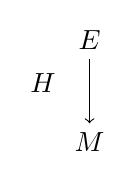
\begin{tikzpicture}[x=1cm,y=1cm,every node/.style={inner sep=1pt}]
\node at (0,.65) {$E$};
\node at (0,-.65) {$M$};
\node at (-.59,.10) {$H$};
\draw[->] (0,.41) -- (0,-.41);
\end{tikzpicture}}\endgroup}
\end{GelfandAdjacentEvidence}
\begin{GelfandAdjacentEvidence}{GELFAND-P000551}{3}

главное рассл. и группа его автоморфизмов

Она проектир. на \(G_1\) со слоем \(G_2\)
\Incomplete{GELFAND-P000551}{bundle-old}{Прямоугольная запись под схемой густо зачёркнута и не читается.}
\end{GelfandAdjacentEvidence}
\begin{GelfandAdjacentEvidence}{GELFAND-P000551}{4}

\[
e^H=H_0\oplus H\oplus S^2(H)\oplus S^3(H)\oplus\ldots
\]
\Unclear{GELFAND-P000551}{fock-upper-marks}{Над \(H,\oplus,S^2(H)\) два горизонтальных штриха и маленькая петля между ними. Их значение и прикрепление не установлены.}
\end{GelfandAdjacentEvidence}
\begin{GelfandAdjacentEvidence}{GELFAND-P000551}{5}

(\(H_0\) — одномерное; \(S^k(H)\) — симметр. степень
\[
1\qquad \xi\qquad\frac{\xi\otimes\xi}{2!}
\qquad\qquad
|\xi|^2=\sum\frac{|\xi_n|^2}{n!}
\]
\Unclear{GELFAND-P000551}{fock-product}{Круглый знак в числителе предположительно читается \(\otimes\).}
\end{GelfandAdjacentEvidence}
\begin{GelfandAdjacentEvidence}{GELFAND-P000551}{6}


\uline{Гуревич.}\quad \uwave{Об ур-[?] К.-д.-Ф. методом Уидема}.
\Unclear{GELFAND-P000551}{gurevich-old}{Окончание после «ур-» переписано. Точное чтение не установлено.}
\end{GelfandAdjacentEvidence}



\Needspace{7\baselineskip}
\begin{GelfandAdjacentEvidence}{GELFAND-P000552}{1}
\SourcePage{GELFAND-P000552}{unlabelled}
\uline{1/\mbox{$\overline{\underline{IV}}$}-74.}\qquad
\uwave{Сем. Гельфанда.}

\uwave{Юра Кобленц.}\qquad\uwave{Об асимптотике соб. значений опер. Лапласа.}

\hspace{2em}(из Ленинграда)\par
\(M\) — замкн. рим. мн-ие, \(\Delta\) — опер. Бельтрами — Лапласа.
\[
\lambda_0=0,\qquad 0\le\lambda_1\le\lambda_2\le\ldots
\qquad\text{— спектр.}
\]
\[
Z(s)=\operatorname{Tr}\exp(-s\Delta)=\sum_i e^{-\lambda_i s}
\]
\[
\Delta f=\frac{1}{\sqrt g}\frac{\partial}{\partial x^i}
\left(\sqrt g\, g^{ij}\frac{\partial f}{\partial x^j}\right),
\qquad\text{где }\underline{g=\det\Vert g_{ij}\Vert},
\]
\Incomplete{GELFAND-P000552}{laplacian-old}{Между знаком равенства и \(1/\sqrt g\) густо зачёркнутая запись. Правый штрих не отделяется уверенно от зачёркивания.}
\end{GelfandAdjacentEvidence}
\begin{GelfandAdjacentEvidence}{GELFAND-P000552}{2}

\[
\uwave{\mbox{$\displaystyle E(m,m',t)=\sum e^{-\lambda_i t}\varphi_i(m)\varphi_i(m').$}}
\]
\Unclear{GELFAND-P000552}{kernel-functions}{В обоих множителях буква предположительно читается \(\varphi\).}
\end{GelfandAdjacentEvidence}
\begin{GelfandAdjacentEvidence}{GELFAND-P000552}{3}

\[
Z(s)=\int E(m,m,s)\,dm
\]

\uline{Minakshisundaram}, \uline{1949}
\[
Z(t)=(4\pi t)^{-n/2}(a_0+a_1t+a_2t^2+\ldots),
\qquad t\to0.
\]
\[
n=\dim M,\qquad a_0=\operatorname{vol} M,\qquad \operatorname{Re}t>0.
\]
\[
a_1=\int_M \frac{\tau}{6}\,dV,
\qquad\text{где }\tau\text{ — скал. кривизна}
\]
\[
\tau=\sum_{\alpha\beta[?]\beta}R_{\alpha\beta[\ldots]}^{\alpha\beta}
\]
\Unclear{GELFAND-P000552}{scalar-indices}{Под знаком суммы читаются начальные \(\alpha\beta\) и конечная \(\beta\), между ними переписанные штрихи. После нижних \(\alpha\beta\) у \(R\) два зачёркнутых знака.}
\end{GelfandAdjacentEvidence}
\begin{GelfandAdjacentEvidence}{GELFAND-P000552}{4}

\[
a_2=\frac1{360}\int\left(2|R|^2-2|\rho|^2+5\tau^2\right)
\]
\(R\) — тензор кривизны; \(\rho\) — тензор Риччи,
\[
\rho_{ij}=\sum_\alpha R_{i\alpha j}^{\alpha}
\]
\Unclear{GELFAND-P000552}{ricci-indices}{После нижнего \(j\) у \(R\) густо переписанный знак. Исходный штрих не читается.}
\end{GelfandAdjacentEvidence}
\begin{GelfandAdjacentEvidence}{GELFAND-P000552}{5}

\[
|R|^2=\sum R_{\alpha\beta\gamma\delta}^2
\qquad\text{в норм. коорд.}\qquad
|R|^2=R_{\alpha\beta\gamma\delta}R^{\alpha\beta\gamma\delta}
\]
\[
|\rho|^2=\rho_{\alpha\beta}\rho^{\alpha\beta}
\]
\[
E(t,m,m')=(4\pi t)^{-n/2}
\left(u_0(m,m')+u_1(m,m')t+u_2(m,m')t^2+\ldots\right)
\]
\uwave{в окр. диагонали}.

\uwave{\mbox{$a_3$} — Sakai и докладчик} (независимо).

\uline{Г.}\quad\uline{Число цел. точек в круге}:
\[
a(r)=\pi r^2+\sum_{\lambda_n}\tau^{1/2}\sin\frac{\tau}{\lambda_n}
\]
\Unclear{GELFAND-P000552}{circle-formula}{В начале формулы буква предположительно \(r\). В обоих местах под знаком суммы широкая волнистая головка, предварительное чтение \(\tau\).}
\end{GelfandAdjacentEvidence}
\begin{GelfandAdjacentEvidence}{GELFAND-P000552}{6}

(\(\lambda_n\) — нули \(\zeta\)-ф-и Римана.) \quad\uwave{mod гипотезы Римана}

\uline{Шнирельман.}\par
В шаре \(\lambda_n\) — длины замкн. биллиардных путей.
\SourceFigure{GELFAND-P000552}{billiard-word}{У первой буквы «шаре» три штриха.}
\end{GelfandAdjacentEvidence}

\[
\sum\delta(\lambda-\lambda_k)*\frac{\varepsilon}{\lambda^2+\varepsilon^2}=f(\lambda)
\]


\Needspace{7\baselineskip}
\begin{GelfandAdjacentEvidence}{GELFAND-P000553}{1}
\SourcePage{GELFAND-P000553}{83}
\[
f(\lambda)=f_0(\lambda)+\sum_k c_k\lambda^{\alpha_k}
\sin(\ell_k\lambda+\omega_k)
\]
Есть экспер. подтверждение (Balian и Bloch)
\Unclear{GELFAND-P000553}{balian-name}{Конец фамилии Balian обведён. Чтение конечной n предположительно.}
\end{GelfandAdjacentEvidence}
\begin{GelfandAdjacentEvidence}{GELFAND-P000553}{2}

(и даже точное утверждение).
\[
\sum e^{i\lambda_k z}=\operatorname{Sp}(e^{-z\Delta}).
\]
\SourceFigure{GELFAND-P000553}{trace-exponent}{Слева в показателе \(i\lambda_k z\), справа \(-z\Delta\).}
\end{GelfandAdjacentEvidence}
\begin{GelfandAdjacentEvidence}{GELFAND-P000553}{3}

\dashuline{продолж. вниз} (из верхн. полуплоск.)

\dashuline{Пробл. близнецов}:
\[
\lambda_{k+1}-\lambda_k>c\lambda_k^{-\nu}
\qquad\text{для общих операторов}
\]
\Unclear{GELFAND-P000553}{gap-exponent}{Буква после минуса имеет две сходящиеся ветви, предварительное чтение \(\nu\).}
\end{GelfandAdjacentEvidence}
\begin{GelfandAdjacentEvidence}{GELFAND-P000553}{4}

\uwave{но на окружности двойные.} (устойчиво асимпт. 2-кр. спектр).

\(T^2\)\qquad \(g_{ij}\sim\delta_{ij}\)\qquad справ. теорема

\uline{Теорема}.
\[
\uwave{\mbox{$\displaystyle\min(\lambda_{k+1}-\lambda_k,\lambda_k-\lambda_{k-1})
< C_N\cdot k^{-N}$}},\qquad \forall N
\]
(Лазуткин, Шнирельман)
\Unclear{GELFAND-P000553}{attribution}{В фамилии «Шнирельман» переписан переход к последним буквам. Исходные штрихи не читаются.}
\end{GelfandAdjacentEvidence}
\begin{GelfandAdjacentEvidence}{GELFAND-P000553}{5}

(малое, но конечное возмущение) — устойч.

Для \(T^3\) это уже \uline{не так}. (\uline{по-видимому}).
\[
\frac{\partial u}{\partial t}=i\sqrt{-\Delta}\,u;\qquad
\left.u\right|_{t=0}=\delta_x
\]
\Unclear{GELFAND-P000553}{wave-numerator}{После \(\partial\) переписанная буква, предположительно \(u\).}
\end{GelfandAdjacentEvidence}
\begin{GelfandAdjacentEvidence}{GELFAND-P000553}{6}

Её реш. \qquad \(u(x,y,t)\)
\[
\sum e^{i\lambda_k t}=\int_M u(x,x,t)\,dx=f(t);
\]
\Unclear{GELFAND-P000553}{trace-time}{В показателе суммы и в последнем аргументе под интегралом обведённые знаки. Оба предположительно \(t\).}
\end{GelfandAdjacentEvidence}
\begin{GelfandAdjacentEvidence}{GELFAND-P000553}{7}

особ. \(u(x,y,t)\) там, где \(\lvert x-y\rvert=t\)

\SourceFigure{GELFAND-P000553}{loop}{%
\par\smallskip
\begingroup\color{black}\GelfandFitDiagram{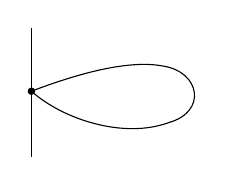
\begin{tikzpicture}[x=1cm,y=1cm]
\draw (0,-.83) -- (0,.80);
\draw (0,0) .. controls (.50,.19) and (1.20,.41) .. (1.67,.32)
  .. controls (2.14,.25) and (2.24,-.26) .. (1.74,-.40)
  .. controls (1.16,-.61) and (.39,-.35) .. (0,0) -- cycle;
\fill (0,0) circle (1.35pt);
\end{tikzpicture}}\endgroup}
\end{GelfandAdjacentEvidence}
\begin{GelfandAdjacentEvidence}{GELFAND-P000553}{8}

при нек. \(t\) происх. бифуркации
\Unclear{GELFAND-P000553}{bifurcation-ending}{Окончание слова «бифуркации» переписано. Чтение предположительно.}
\end{GelfandAdjacentEvidence}

особ. движ. со скор. 1



\clearpage\section*{Глава 8}

\Needspace{7\baselineskip}
\begin{GelfandAdjacentEvidence}{GELFAND-P000554}{1}
\SourcePage{GELFAND-P000554}{unlabelled}
\uline{2/\mbox{$\overline{\underline{IX}}$}-74.}\qquad
\uuline{Сем. Гельфанда}\quad (32-й год работы семинара)

\uline{Джусти}.

1. \uwave{Singularities} [зачёркнуто] \uwave{and regularity}
\Unclear{GELFAND-P000554}{title-old}{Между «Singularities» и «and» перечёркнутые штрихи. Исходная запись не читается.}
\end{GelfandAdjacentEvidence}
\begin{GelfandAdjacentEvidence}{GELFAND-P000554}{2}

[зачёркнуто] of solutions of non-linear elliptic (and parabolic) systems.
\Unclear{GELFAND-P000554}{line-prefix-old}{Перед «of solutions» отдельная зачёркнутая запись. Чтение не установлено.}
\end{GelfandAdjacentEvidence}
\begin{GelfandAdjacentEvidence}{GELFAND-P000554}{3}

\uwave{Nash, De giorgi, Moser}. — Regularity: 1 equation linear
\sout{di\ldots} with discont. coeff. (Höld. coeff.)
\(\Rightarrow\) regul. for non linear with smooth coeff.
\Unclear{GELFAND-P000554}{linear-old}{Перед «with» зачёркнуты буквы. Начало предположительно «di».}
\end{GelfandAdjacentEvidence}
\begin{GelfandAdjacentEvidence}{GELFAND-P000554}{4}

\uline{Systems} — [зачёркнуто] \uwave{неверно}. Быв. ср. коэфф. и несгр. решения
\Unclear{GELFAND-P000554}{systems-old}{После тире перед «неверно» густо перечёркнутый знак.}
\end{GelfandAdjacentEvidence}
\begin{GelfandAdjacentEvidence}{GELFAND-P000554}{5}

\Unclear{GELFAND-P000554}{systems-caption}{Сокращения до «коэфф.» и «решения» предположительно читаются «Быв. ср.» и «несгр.».}
\end{GelfandAdjacentEvidence}
\begin{GelfandAdjacentEvidence}{GELFAND-P000554}{6}

1968 Miranda, Giusti — сист. с аналит. коэфф. с разр. решениями
\Unclear{GELFAND-P000554}{giusti-name}{Начало фамилии Giusti переписано, исходные штрихи не читаются.}
\end{GelfandAdjacentEvidence}
\begin{GelfandAdjacentEvidence}{GELFAND-P000554}{7}

\hfill\rule{1.4cm}{.35pt}\enspace\(\cdot\)\enspace\rule{1.4cm}{.35pt}\par
\(\Sigma\) — singular set.
\begin{align*}
&(1)\quad \Sigma\text{ closed}\\
&(2)\quad \dim\Sigma<n-2
\end{align*}
\hfill\rule{1.4cm}{.35pt}\enspace\(\cdot\)\enspace\rule{1.4cm}{.35pt}\par

2. \uwave{Boundary value problems. for surfaces of prescribed mean curvature}.
\[
u:\Omega\longrightarrow\mathbb R \qquad \operatorname{graph}u=S
\]
\SourceFigure{GELFAND-P000554}{domain-outline}{%
\par\smallskip
\begingroup\color{black}\GelfandFitDiagram{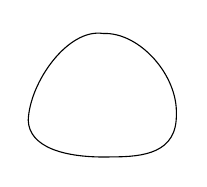
\begin{tikzpicture}[x=.95cm,y=.95cm]
\draw (.04,.52) .. controls (.06,1.03) and (.57,1.75) .. (1.04,1.68)
  .. controls (1.53,1.70) and (2.04,1.12) .. (2.02,.60)
  .. controls (2.03,.08) and (1.58,.03) .. (1.16,.03)
  .. controls (.50,.01) and (.05,.17) .. (.04,.52) -- cycle;
\end{tikzpicture}}\endgroup}
\end{GelfandAdjacentEvidence}
\begin{GelfandAdjacentEvidence}{GELFAND-P000554}{8}

\SourceFigure{GELFAND-P000554}{graph-sketch}{%
\par\smallskip
\begingroup\color{black}\GelfandFitDiagram{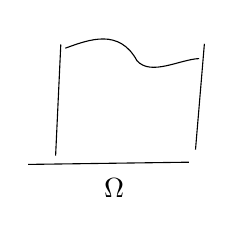
\begin{tikzpicture}[x=.94cm,y=.94cm,every node/.style={inner sep=1pt}]
\draw (0,0) -- (2.17,.03);
\draw (.37,.12) -- (.44,1.62);
\draw (2.26,.20) -- (2.38,1.63);
\draw (.50,1.57) .. controls (.83,1.69) and (1.23,1.84) .. (1.47,1.40)
  .. controls (1.66,1.19) and (2.05,1.42) .. (2.31,1.43);
\node[below] at (1.16,-.15) {$\Omega$};
\end{tikzpicture}}\endgroup}
\end{GelfandAdjacentEvidence}
\begin{GelfandAdjacentEvidence}{GELFAND-P000554}{9}

\[
H(x)=\frac{1}{n}\sum\frac{\partial}{\partial x_i}
\left(\frac{\partial u/\partial x_i}{\sqrt{1+|\operatorname{grad}u|^2}}\right)
\]
\(H\) не очень велико (иначе неразрешимо). Зависит от геометрии области, ф-и \(H(x)\) и т. д.

Это и будет в следующий раз.

\uuline{С. П. Новиков.} (и Дубровин).

Абелево мн-зие \(\xi_1,\ldots,\xi_{2n}\) — базис в \(\mathbb C^n\) (над \(\mathbb R\)),
\(T^{2n}\) — соотв. тор. Пусть абелево мн-зие (алгебраич. мн-зие).

Как описать все торы?

\uuline{\mbox{$n=2$}}\qquad \uwave{уже нетривиально}.
\[
y^2=P_{2n+1}(x)\qquad\text{рим. поверхность}\quad\Rightarrow\quad\text{тор.}
\]
\Incomplete{GELFAND-P000554}{cohomology-old}{Перед \(H^1\) зачёркнутая запись с предположительным началом «Вид…». Остальное не читается.}
\end{GelfandAdjacentEvidence}
\begin{GelfandAdjacentEvidence}{GELFAND-P000554}{10}

\[
\underbrace{H^1(R,\mathbb C)/H^1(R,\mathbb Z)}_{\text{тор такой}}
\qquad \uwave{\mbox{$R\longrightarrow J^{2n}(R).$}}\quad(\text{тор})
\]
\[
k=0,\ldots,n-1,\qquad
\boxed{\omega_k=\frac{x^k\,dx}{\sqrt{P_{2n+1}(x)}}}
\quad\longleftarrow\quad\text{всюду регулярные дифференциалы}.
\]
Базис — формы \(\omega_k\).
\[
P_{2n+1}(x)=\prod(x-x_\alpha).
\]
Всё опр. набором корней.

\SourceFigure{GELFAND-P000554}{moduli-maps}{%
\par\smallskip
\begingroup\color{black}\GelfandFitDiagram{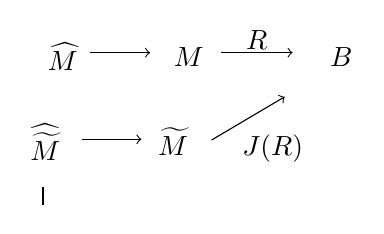
\begin{tikzpicture}[x=1cm,y=1cm,every node/.style={inner sep=1pt}]
\node (cover) at (0,0) {$\widehat M$};
\node (surfaces) at (1.60,0) {$M$};
\node (base) at (3.54,0) {$B$};
\draw[->] (.35,.05) -- (1.11,.05);
\draw[->] (2.01,.05) -- node[above] {$R$} (2.92,.05);
\node at (-.22,-1.09) {$\widehat{\widetilde M}$};
\node at (1.40,-1.08) {$\widetilde M$};
\draw[->] (.25,-1.05) -- (1.00,-1.05);
\draw[->] (1.89,-1.06) -- (2.82,-.51);
\node[right] at (2.24,-1.17) {$J(R)$};
\draw (-.25,-1.65) -- (-.25,-1.89);
\end{tikzpicture}}\endgroup\par\smallskip
Нижняя наклонная стрелка заканчивается левее и ниже верхней буквы B. Точная связь не установлена.}
\end{GelfandAdjacentEvidence}


\(M\) — совок. рим. поверхностей

\(B\) — верхняя полуплоскость Зигеля

(накрытие мн-зия модулей).

по набору корней строится многочлен, а по нему тор.


\Needspace{7\baselineskip}
\begin{GelfandAdjacentEvidence}{GELFAND-P000555}{1}
\SourcePage{GELFAND-P000555}{unlabelled}
\begin{gather*}
p_1,p_2,q_1,q_2,c,d.\qquad \mathbb C^6\text{ или }\mathbb C^4_{c,d}\\
J_1=p_1p_2+V(q_1,q_2)\\
J_2=p_1^2-2q_1p_1p_2+2(q_2-c)p_2^2+\mathcal D(q_1,q_2)\\
\Omega=\sum_{\alpha=1}^{2}dp_\alpha\wedge dq_\alpha.
\end{gather*}
\(\langle J_1,J_2\rangle\equiv0.\) \quad ск. Пуассона
\[
V=-\left(\frac{q_2^2}{2}+\frac52q_1^2q_2+\frac52q_1^4\right)+c_1q_1^2-d_1q_1
\]
\Unclear{GELFAND-P000555}{potential-symbol}{Знак перед равенством переписан. Видны две верхние ветви, предварительное чтение \(V\).}
\end{GelfandAdjacentEvidence}
\begin{GelfandAdjacentEvidence}{GELFAND-P000555}{2}

\[
\mathcal D=q_1^5+2c_1q_1^3+d_1q_1^2-4q_1q_2^2+4c_1q_1q_2-2d_1q_2
\]
\[
[X_{J_1},X_{J_2}]=0.\quad\text{Получ. 2 коммут. поля.}
\]
Соотв. орбиты — абелево мн-зие
\[
\left.\underline{\begin{aligned}
J_1&=\mathrm{const}\\
J_2&=\mathrm{const}
\end{aligned}}\right\}\quad\text{\uuline{тор.}}
\]
\Unclear{GELFAND-P000555}{orbit-old}{Слева от двух равенств зачёркнута запись с начертанием, похожим на \(J\). Остальное не читается.}
\end{GelfandAdjacentEvidence}
\begin{GelfandAdjacentEvidence}{GELFAND-P000555}{3}

\uwave{Следствие}: совок. всех их — унирац. многообразие.
\[
R:\quad y^2=x^5+\frac{c_1}{4}x^3-\frac{d_1}{16}x^2+
\left(\frac{J_1}{32}+\frac{c_1^2}{4}\right)x+\frac{J_2}{2^8}+\frac{c_1d_1}{2^7}
\]
\hfill\rule{1.4cm}{.35pt}\enspace\(\cdot\)\enspace\rule{1.4cm}{.35pt}\par
\(R\) — рим. пов., \quad \(S^nR\) — симметр. степень \(R\).

\((J_1,\ldots,J_n)\) и симметризация.
\Unclear{GELFAND-P000555}{symmetric-label}{В строке перед «и симметризация» обе буквы с крюками. Предположительное чтение \(J\).}
\end{GelfandAdjacentEvidence}
\begin{GelfandAdjacentEvidence}{GELFAND-P000555}{4}

\begin{gather*}
S^nR\longrightarrow J(R).\\
(P_1,\ldots,P_n)\xrightarrow{A}(\alpha_1,\ldots,\alpha_n)
\qquad\text{отобр. Абеля.}
\end{gather*}
(\uline{Теор. Абеля} — это изоморфизм).
\SourceFigure{GELFAND-P000555}{abel-paths}{%
\par\smallskip
\begingroup\color{black}\GelfandFitDiagram{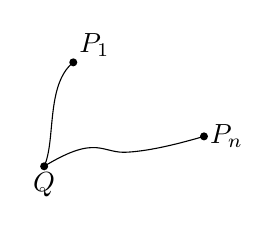
\begin{tikzpicture}[x=1cm,y=1cm,every node/.style={inner sep=2pt}]
\draw (0,0) .. controls (.15,.32) and (.02,1.04) .. (.37,1.32);
\draw (0,0) .. controls (.69,.42) and (.73,.15) .. (1.07,.18)
  .. controls (1.37,.20) and (1.72,.29) .. (2.03,.38);
\fill (0,0) circle (1.45pt) node[below] {$Q$};
\fill (.37,1.32) circle (1.45pt) node[above right] {$P_1$};
\fill (2.03,.38) circle (1.45pt) node[right] {$P_n$};
\end{tikzpicture}}\endgroup\par\smallskip
Верхняя кривая утолщается у точки \(P_1\). Наконечник стрелки не различается.}
\end{GelfandAdjacentEvidence}
\begin{GelfandAdjacentEvidence}{GELFAND-P000555}{5}

\[
(P_1,\ldots,P_n)\longrightarrow
\left(\underbrace{\sum_{k=1}^{n}\oint_Q^{P_k}\omega_s}
_{\substack{\vert\vert\\ \alpha_s}}\right)
\]
\SourceFigure{GELFAND-P000555}{abel-integral}{На знаке интеграла видна петля. Под скобкой над \(\alpha_s\) стоят два коротких штриха.}
\end{GelfandAdjacentEvidence}
\begin{GelfandAdjacentEvidence}{GELFAND-P000555}{6}

\[
L=-\frac{d^2}{dx^2}+u(x),
\]
\uwave{\mbox{$u(x+T)=u(x)$}}\quad или\quad \uwave{квазипериодичн}.
\[
\text{Соб. ф-я}\qquad
\uwave{\mbox{$L\Psi(x,E)=E\Psi,$}}
\]
\[
\Psi(x+T)=\lambda\Psi(x),\qquad |\lambda|=1,\qquad\lambda=e^{ip(E)}
\]
(Блоховские соб. ф-и)

Для почти периодичн. [зачёркнуто] ансамбль таких соб. ф-й не обр. полную систему.
\Incomplete{GELFAND-P000555}{almost-periodic-old}{После «периодичн.» короткая густо зачёркнутая запись.}
\end{GelfandAdjacentEvidence}

\[
\left.\Psi\right|_{x_0}=1 \quad\text{— нормировка}
\]
\[
\Psi(x,E,x_0)\qquad (\Psi,\overline\Psi)\quad\text{— 2 соб. ф-и.}
\]
по \(E\) ветвится в концах отр. спектра. Получ. рим. пов. беск. рода. 2 листа, т. к. 2 соб. ф-и.


\Needspace{7\baselineskip}
\begin{GelfandAdjacentEvidence}{GELFAND-P000556}{1}
\SourcePage{GELFAND-P000556}{unlabelled}
Мн-во потенц. с зад. зонной структурой — мн-зие Якоби этой рим. поверхности (есть ф-лы)
\Unclear{GELFAND-P000556}{zonal-overwrite}{В слове «зонной» первые штрихи переписаны.}
\end{GelfandAdjacentEvidence}
\begin{GelfandAdjacentEvidence}{GELFAND-P000556}{2}

\SourceFigure{GELFAND-P000556}{spectrum-line}{%
\par\smallskip
\begingroup\color{black}\GelfandFitDiagram{\begin{tikzpicture}[x=.62cm,y=.66cm,every node/.style={inner sep=1pt}]
\draw (0,0) -- (6.7,0);
\draw[line width=1.5pt] (0,0) -- (.90,0);
\draw[line width=1.5pt] (2.22,0) -- (3.00,0);
\draw[line width=1.5pt] (4.76,0) -- (6.70,0);
\foreach \position in {0,.90,2.22,3.00,4.76}
  \draw (\position,-.12) -- (\position,.12);
\node[below] at (0,-.12) {$x_1$};
\node[below] at (.90,-.12) {$x_2$};
\node[below] at (4.76,-.12) {$x_{2n+1}$};
\node[right] at (6.82,0) {\uuline{спектр.}};
\end{tikzpicture}}\endgroup}
\end{GelfandAdjacentEvidence}
\begin{GelfandAdjacentEvidence}{GELFAND-P000556}{3}

Потенц. с зад. зонной структурой — соотв. тор (мн-зие Якоби).
\hfill\(\cdots\cdots\cdots\cdots\cdots\cdots\cdots\cdots\)\par

\uline{9/\mbox{$\overline{\underline{IX}}$}-74}\enspace.\qquad\uline{Сем. Гельфанда.}

\uline{Бесага} (\uwave{Варшава}).\quad \uwave{\mbox{$Z$}-множества Андерсона и их приложения}.
\hfill (R. D. Anderson)\par
\(X\) — полное метриз. пр-во. \quad \(A\subset X,\ \overline{A}=A\).

\(A\) наз. \(Z\)-мн-вом, если \(\forall\) непр. отобр.
\[
f:\underbrace{I^\infty}_{\text{гильб. куб.}}\longrightarrow X,\qquad
\forall\varepsilon>0,\qquad
\exists g:I^\infty\longrightarrow X\setminus A,\qquad
\rho(f,g)<\varepsilon.
\]
\[
\underline{Q=[-1,1]^\infty,\qquad P=(-1,1)^\infty.}
\qquad(Q\setminus P)\text{ — \(Z\)-мн-во}
\]
\uline{Св-ва}: \(1^\circ\). Если \(A,B\) — \(Z\)-мн-ва (в \(Q\)),
то \(f:A\xrightarrow{\sim} B\) продолж. до \sout{гомео} гомеом. всего пр-ва.
\Unclear{GELFAND-P000556}{property-number}{У \(1^\circ\) цифра густо переписана. Кружок и точка различимы.}
\end{GelfandAdjacentEvidence}
\begin{GelfandAdjacentEvidence}{GELFAND-P000556}{4}

\Unclear{GELFAND-P000556}{extension-old}{Зачёркнутое начало перед «гомеом.» предположительно читается «гомео».}
\end{GelfandAdjacentEvidence}
\begin{GelfandAdjacentEvidence}{GELFAND-P000556}{5}


\uwave{\mbox{$Z_\sigma$}-мн-во} — счётное объед. \(Z\)-мн-в.

\(2^\circ\). Сущ. максимальное \(Z_\sigma\)-мн-во
\hfill\rule{1.4cm}{.35pt}\enspace\(\cdot\)\enspace\rule{1.4cm}{.35pt}\par

\uline{Гельфанд}

Рассм. \(\mathbb R^\infty\) в тих. топологии и пр-во \(S\) лучей, [зачёркнуто] вых. из 0 в ест. топологии.
Док., что на \(S\) любая непр. ф-я [зачёркнуто] \uline{const}
\Incomplete{GELFAND-P000556}{rays-old}{Между «лучей» и «вых.» густо зачёркнутая запись.}
\end{GelfandAdjacentEvidence}
\begin{GelfandAdjacentEvidence}{GELFAND-P000556}{6}

\Unclear{GELFAND-P000556}{constant-old}{Перед «const» небольшой зачёркнутый знак. Чтение не установлено.}
\end{GelfandAdjacentEvidence}
\begin{GelfandAdjacentEvidence}{GELFAND-P000556}{7}

(Гельф., Фукс. Функц. анализ I, 4).
\hfill\rule{1.4cm}{.35pt}\enspace\(\cdot\)\enspace\rule{1.4cm}{.35pt}\par
\uline{Бесага}. Все сепараб. пр-ва Фреше гомеоморфны.

\uuline{Джусти.}\qquad \(\Omega\subset\mathbb R^n\)
\SourceFigure{GELFAND-P000556}{hatched-domain}{%
\par\smallskip
\begingroup\color{black}\GelfandFitDiagram{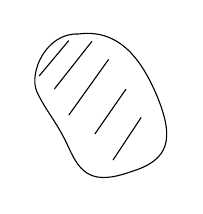
\begin{tikzpicture}[x=.92cm,y=.92cm]
\draw (.13,1.20) .. controls (.01,1.48) and (.27,2.02) .. (.70,2.00)
  .. controls (1.29,2.08) and (1.59,1.61) .. (1.79,1.14)
  .. controls (2.03,.55) and (1.96,.26) .. (1.43,.10)
  .. controls (.90,-.09) and (.73,.07) .. (.57,.43)
  .. controls (.40,.80) and (.27,.91) .. (.13,1.20) -- cycle;
\draw (.16,1.42) -- (.57,1.91) (.37,1.24) -- (.89,1.90)
      (.57,.88) -- (1.12,1.65) (.93,.62) -- (1.36,1.24)
      (1.18,.26) -- (1.57,.85);
\end{tikzpicture}}\endgroup}
\end{GelfandAdjacentEvidence}
\begin{GelfandAdjacentEvidence}{GELFAND-P000556}{8}

\[
\left\{\begin{aligned}
\sum_{i=1}^{n}D_i\left\{\frac{D_i u}{\sqrt{1+|Du|^2}}\right\}
&=-H(x,u)\quad\text{в }\Omega,\\
u&=\phi\quad\text{на }\partial\Omega
\end{aligned}\right.
\qquad D_i=\frac{\partial}{\partial x_i}.
\]
\(n\)-кр. средн. кривизна \(=\) лев. часть ур-я

\(\underline{H\equiv0}\quad\Rightarrow\quad\text{minimal surface.}\)
\SourceFigure{GELFAND-P000556}{graph-cylinder}{%
\par\smallskip
\begingroup\color{black}\GelfandFitDiagram{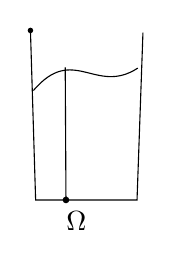
\begin{tikzpicture}[x=.94cm,y=.92cm,every node/.style={inner sep=1pt}]
\draw (0,2.34) -- (.07,0) -- (1.44,0) -- (1.52,2.31);
\draw (.04,1.51) .. controls (.58,2.16) and (.88,1.44) .. (1.45,1.82);
\draw (.47,1.83) -- (.48,0);
\fill (.48,0) circle (1.2pt);
\fill (0,2.34) circle (1pt);
\node[below] at (.62,-.12) {$\Omega$};
\end{tikzpicture}}\endgroup\par\smallskip
У нижнего конца внутреннего вертикального штриха тёмная отметка. Её форма неразличима.}
\end{GelfandAdjacentEvidence}
\begin{GelfandAdjacentEvidence}{GELFAND-P000556}{9}

\uline{Example 1}.\quad \(\Omega,\quad n=2,\quad H=0\)
\SourceFigure{GELFAND-P000556}{annulus}{%
\par\smallskip
\begingroup\color{black}\GelfandFitDiagram{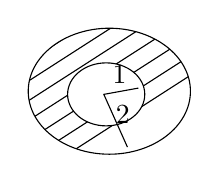
\begin{tikzpicture}[x=1cm,y=1cm,every node/.style={inner sep=1pt}]
\begin{scope}
\pgfseteorule
\clip (0,0) ellipse (1.03 and .80) (-.04,-.04) ellipse (.49 and .40);
\foreach \height in {-1.2,-.95,-.70,-.45,-.20,.05,.30,.55,.80}
  \draw (-1.15,\height) -- (1.12,{\height+1.46});
\end{scope}
\draw (0,0) ellipse (1.03 and .80) (-.04,-.04) ellipse (.49 and .40);
\draw (.37,.04) -- (-.07,-.04) -- (.23,-.71);
\node at (.13,.21) {$1$};
\node at (.17,-.30) {$2$};
\end{tikzpicture}}\endgroup\par\smallskip
circular annulus. Подписи 1 и 2 стоят у двух радиальных штрихов.}
\end{GelfandAdjacentEvidence}
\begin{GelfandAdjacentEvidence}{GELFAND-P000556}{10}

\[
\phi=\begin{cases}
0&|x|=2\\
M&|x|=1
\end{cases}
\]
\uwave{Solution}:\quad \(u(r),\qquad \uwave{\mbox{$r=|x|$}}.\)
\begin{gather*}
u(r)=c\log\frac{2+\sqrt{4-c^2}}{r+\sqrt{r^2-c^2}},\qquad 0\le c\le1,\\
u(1)=M\quad\Rightarrow\quad u(1)\le\log(2+\sqrt3)=M_0.
\end{gather*}
\Unclear{GELFAND-P000556}{radial-overwrites}{Начальные штрихи у \(u(r)\) и \(u(1)\) густо переписаны. Под ними прежнее начертание не читается.}
\end{GelfandAdjacentEvidence}



\Needspace{7\baselineskip}
\begin{GelfandAdjacentEvidence}{GELFAND-P000557}{1}
\SourcePage{GELFAND-P000557}{unlabelled}
При \(M>M_0\) решений нет.

\uline{Экспер. проверка}: мыльн. пузырь\par
осторожно поднимаем \uline{палку}
\hfill\uwave{steak.}\par
\SourceFigure{GELFAND-P000557}{english-word}{Под «палку» написано «steak.» с волнистой чертой.}
\end{GelfandAdjacentEvidence}
\begin{GelfandAdjacentEvidence}{GELFAND-P000557}{2}

\SourceFigure{GELFAND-P000557}{soap-surfaces}{%
\par\smallskip
\begingroup\color{black}\GelfandFitDiagram{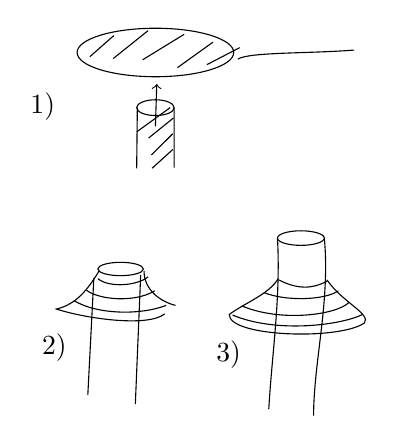
\begin{tikzpicture}[x=.85cm,y=.77cm,every node/.style={inner sep=1pt}]
\node[left] at (.30,1.05) {1)};
\draw (1.75,1.94) ellipse (1.17 and .40);
\draw (2.98,1.83) .. controls (3.15,1.95) and (4.05,1.92) .. (4.72,1.98);
\draw (.77,1.87) -- (1.13,2.22) (1.12,1.84) -- (1.64,2.30)
      (1.56,1.82) -- (2.18,2.24) (2.08,1.69) -- (2.61,2.11)
      (2.52,1.74) -- (3.01,2.02);
\draw (1.47,.03) -- (1.48,1.03) (2.03,.04) -- (2.03,1.03);
\draw (1.75,1.03) ellipse (.28 and .13);
\draw (1.47,.63) -- (1.97,1.03) (1.65,.53) -- (2.02,.86)
      (1.69,.25) -- (2.01,.60) (1.70,.03) -- (2.01,.34);
\draw[->] (1.75,.72) -- (1.77,1.42);
\begin{scope}[yshift=-3.05cm]
\node at (.24,1.03) {2)};
\draw (1.23,2.33) ellipse (.34 and .11);
\draw (.91,2.30) .. controls (.74,1.99) and (.56,1.74) .. (.27,1.67)
  .. controls (.68,1.52) and (1.63,1.36) .. (1.89,1.59);
\draw (1.58,2.30) .. controls (1.58,1.98) and (1.83,1.79) .. (2.05,1.73);
\draw (.89,2.17) .. controls (1.07,2.01) and (1.49,2.06) .. (1.64,2.20)
      (.72,1.98) .. controls (.91,1.82) and (1.44,1.77) .. (1.74,1.97)
      (.53,1.81) .. controls (.89,1.57) and (1.54,1.57) .. (1.91,1.73);
\draw (.83,2.18) -- (.74,.25) (1.53,2.23) -- (1.45,.10);
\begin{scope}[xshift=2.23cm]
\node at (.22,.92) {3)};
\draw (1.30,2.84) ellipse (.35 and .12);
\draw (.95,2.84) .. controls (1.00,1.87) and (.87,.95) .. (.82,.02);
\draw (1.65,2.84) .. controls (1.74,1.80) and (1.49,.80) .. (1.49,-.09);
\draw (.96,2.17) .. controls (.82,1.91) and (.46,1.77) .. (.23,1.58)
  .. controls (.22,1.21) and (1.87,1.15) .. (2.25,1.44)
  .. controls (2.35,1.59) and (1.92,1.78) .. (1.69,2.15);
\draw (.97,2.15) .. controls (1.25,1.99) and (1.48,2.00) .. (1.69,2.13)
      (.75,1.94) .. controls (1.09,1.79) and (1.67,1.82) .. (1.86,1.97)
      (.42,1.72) .. controls (1.00,1.45) and (1.83,1.57) .. (2.02,1.78)
      (.28,1.57) .. controls (.95,1.26) and (1.92,1.41) .. (2.22,1.58);
\end{scope}
\end{scope}
\end{tikzpicture}}\endgroup}
\end{GelfandAdjacentEvidence}
\begin{GelfandAdjacentEvidence}{GELFAND-P000557}{3}


если провол. кольцо, то
\SourceFigure{GELFAND-P000557}{wire-ring}{%
\par\smallskip
\begingroup\color{black}\GelfandFitDiagram{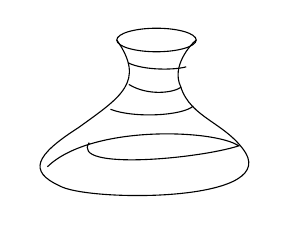
\begin{tikzpicture}[x=.9cm,y=.83cm]
\draw (0,1.89) ellipse (.56 and .18);
\draw (-.56,1.89) .. controls (-.15,1.25) and (-.50,1.02) .. (-1.10,.55)
  .. controls (-1.72,.12) and (-1.81,-.12) .. (-1.37,-.34)
  .. controls (-1.00,-.58) and (1.67,-.61) .. (1.26,.16)
  .. controls (.98,.63) and (.48,.69) .. (.34,1.18)
  .. controls (.21,1.48) and (.47,1.81) .. (.56,1.89);
\draw (-.40,1.54) .. controls (-.17,1.42) and (.27,1.43) .. (.42,1.48)
      (-.39,1.21) .. controls (-.12,1.03) and (.24,1.08) .. (.35,1.17)
      (-.65,.83) .. controls (-.32,.69) and (.37,.73) .. (.52,.88);
\draw (-1.54,-.05) .. controls (-.92,.60) and (.83,.52) .. (1.16,.27)
  .. controls (.59,.07) and (-1.22,-.11) .. (-.95,.32);
\end{tikzpicture}}\endgroup}
\end{GelfandAdjacentEvidence}
\begin{GelfandAdjacentEvidence}{GELFAND-P000557}{4}


\uline{Example 2}.\quad \(n=1,\quad \Omega=(-1,1)\)
\[
\uwave{\mbox{$u=3x^{1/3}$}}
\]
\Unclear{GELFAND-P000557}{cube-root-symbol}{Начальная буква переписана. Окончательный контур предположительно читается \(u\).}
\end{GelfandAdjacentEvidence}
\begin{GelfandAdjacentEvidence}{GELFAND-P000557}{5}

\[
\left(\frac{u'}{\sqrt{1+u'^2}}\right)'=
\underbrace{-\frac23 x^{1/3}\left(1+x^{4/3}\right)^{-3/2}}_{\text{\uline{непрер.}}}
\]
\SourceFigure{GELFAND-P000557}{derivative-power}{У первого \(x\) показатель \(1/3\), у второго \(x\) — \(4/3\).}
\end{GelfandAdjacentEvidence}
\begin{GelfandAdjacentEvidence}{GELFAND-P000557}{6}

[зачёркнуто] \(u\) — недифф.
\Unclear{GELFAND-P000557}{nondifferentiable-old}{У зачёркнутой записи возможно начало «об…». Конец не разбирается.}
\end{GelfandAdjacentEvidence}
\begin{GelfandAdjacentEvidence}{GELFAND-P000557}{7}

\[
\uwave{\mbox{$u(-1)=-3,\qquad u(1)=3$}}
\]
Пусть
\[
u(-1)=3,\qquad u(1)=3+A
\]
\SourceFigure{GELFAND-P000557}{boundary-sign}{После «Пусть» написано \(u(-1)=3\).}
\end{GelfandAdjacentEvidence}

\begin{gather*}
\frac{u'}{\sqrt{1+u'^2}}=(1+x^{4/3})^{-1/2}\\
u'\le x^{-2/3}\\
u(x)\le -3+\int_{-1}^{x}t^{-2/3}\,dt=3x^{1/3}
\end{gather*}
\hfill\rule{1.4cm}{.35pt}\enspace\(\cdot\)\enspace\rule{1.4cm}{.35pt}\par
\[
\mathcal F(u)=\int_\Omega\sqrt{1+|Du|^2}\,dx+\int_\Omega\lambda(x,u)\,dx
\]
\hfill Надо найти \uuline{min}.\par
\[
\lambda(x,t)=\int_0^t H(x,s)\,ds
\]
При усл. \(|u'|\le K\) есть \uwave{min}. (иначе нет).

\(u_k\) — реш. Пусть \(k\to+\infty\). \qquad \(u_k\to u_0\) ?
\hfill\rule{1.4cm}{.35pt}\enspace\(\cdot\)\enspace\rule{1.4cm}{.35pt}\par
\(u\) — Lip-contin. solut.\qquad \(A\subset\Omega\)
\begin{gather*}
\int_A H(x)\,dx=\int_{\partial A} n_i\frac{D_i u}{\sqrt{1+|Du|^2}}\,dH_{n-1}\\
\left|\int_A H(x)\,dx\right|\le(1-\varepsilon_0)H_{n-1}(\partial A)\\
\boxed{1-\varepsilon_0=\sup_{\Omega}\frac{|Du|}{\sqrt{1+|Du|^2}}.}
\end{gather*}
\uwave{Поэтому \mbox{$H$} не очень велико}.
\hfill\rule{1.4cm}{.35pt}\enspace\(\cdot\)\enspace\rule{1.4cm}{.35pt}\par


\Needspace{7\baselineskip}
\begin{GelfandAdjacentEvidence}{GELFAND-P000558}{1}
\SourcePage{GELFAND-P000558}{unlabelled}
\(\textcircled{1}\qquad H^{1,1}=W_1^1\qquad\parallel\)
\[
\mathcal F(u)=\int_\Omega\sqrt{1+|Du|^2}\,dx+
\int_\Omega\lambda(x,u)\,dx+
\int_{\partial\Omega}|u-\phi|\,dH_{n-1}
\]
\(BV(\Omega)\) \(=\) \(L^1\)-ф-и, у к-рых 1-е произв. — меры (Радона).
\[
\begin{gathered}
\text{т. е.}\quad f\in BV \iff f\in L^1,\\
\sup\left\{\int_\Omega f\operatorname{div}\vec g\,dx,\quad
\vec g\in C_0^1(\Omega),\ |g|\le1\right\}<+\infty
\end{gathered}
\]
\[
\sup=\int_\Omega \overset{\vert\vert}{|Df|}\,dx
\]
\Unclear{GELFAND-P000558}{variation-bars}{Над \(Df\) две отдельные черты. Слева от них зачёркнутый знак не читается.}
\end{GelfandAdjacentEvidence}
\begin{GelfandAdjacentEvidence}{GELFAND-P000558}{2}

\uwave{Площадь}\quad \underline{\(f\in BV.\)}
\[
\begin{aligned}
\mathcal A(f)&=\int\sqrt{1+|Df|^2}\,dx\underset{\mathrm{def}}{=}\\
&\sup\left\{\int_\Omega(g_0+f\operatorname{div}\vec g)\,dx,\quad
g_0,g\in C_0^1,\quad g_0^2+|g|^2\le1\right\}.
\end{aligned}
\]
\Unclear{GELFAND-P000558}{area-test}{Левая черта при \(g\) слита с буквой. Предположительно \(|g|^2\).}
\end{GelfandAdjacentEvidence}
\begin{GelfandAdjacentEvidence}{GELFAND-P000558}{3}

\uwave{area}.

\((\mathcal A f)\) lower semicont. with respect to \(L^1\) \sout{cont\ldots y}.
\Unclear{GELFAND-P000558}{semicontinuity-old}{В зачёркнутом английском слове предположительно читаются «cont…y». Полное слово не установлено.}
\end{GelfandAdjacentEvidence}
\begin{GelfandAdjacentEvidence}{GELFAND-P000558}{4}

\textcircled{2} Bounded sets in \(BV\) are relatively compact in \(L_1\)
\par\noindent\(\cdots\cdots\cdots\cdots\cdots\cdots\cdots\cdots\cdots\)

\uuline{Дубровин}.
\[
L=-\frac{d^2}{dx^2}+u(x),\qquad
\uwave{\mbox{$u(x+T)=u(x)$}}
\]
\(E\) — спектр. параметр.
\SourceFigure{GELFAND-P000558}{spectral-lines}{%
\par\smallskip
\begingroup\color{black}\GelfandFitDiagram{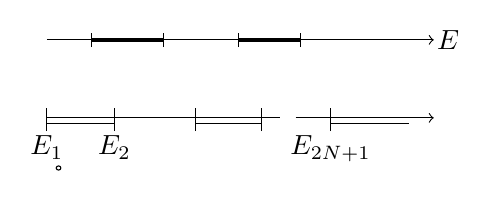
\begin{tikzpicture}[x=.78cm,y=.7cm,every node/.style={inner sep=1pt}]
\draw[->] (0,0) -- (6.30,0) node[right] {$E$};
\draw[line width=1.35pt] (.73,0) -- (1.90,0) (3.12,0) -- (4.13,0);
\foreach \x in {.73,1.90,3.12,4.13}
  \draw (\x,-.13) -- (\x,.13);
\begin{scope}[yshift=-.99cm]
\draw (0,0) -- (3.80,0);
\draw[->] (4.05,0) -- (6.30,0);
\draw (0,-.11) -- (1.10,-.11) (2.42,-.11) -- (3.49,-.11)
      (4.62,-.11) -- (5.90,-.11);
\foreach \x in {0,1.10,2.42,3.49,4.62}
  \draw (\x,-.24) -- (\x,.18);
\node[below] at (0,-.27) {$E_1$};
\draw (.19,-.91) circle (.038);
\node[below] at (1.10,-.27) {$E_2$};
\node[below] at (4.62,-.27) {$E_{2N+1}$};
\end{scope}
\end{tikzpicture}}\endgroup\par\smallskip
Под \(E_1\) маленькая незакрашенная петля. Её значение не установлено.}
\end{GelfandAdjacentEvidence}
\begin{GelfandAdjacentEvidence}{GELFAND-P000558}{5}

Иногда лакуны исчезают.

Пусть \(u(x)\) — конечнозонный потенциал

Пусть \(R(E)=\prod(E-E_i)\)

Рассм. рим. пов. ф-и \(\sqrt{R(E)}\) — обозн. \(\Gamma_N\).

\uwave{блоховские соб. ф-и аналит. прод. на \mbox{$\Gamma_N\setminus\infty$}} [зачёркнуто]
\Incomplete{GELFAND-P000558}{continuation-old}{Справа скобочная запись густо зачёркнута и не читается.}
\end{GelfandAdjacentEvidence}
\begin{GelfandAdjacentEvidence}{GELFAND-P000558}{6}

\hfill\underline{(мероморфно)}\par
\uwave{\mbox{$N$} — род.}

и имеет \(N\) полюсов и \(N\) нулей

\uwave{блоховск. соб. ф-я:} \(\Psi(x,E,x_0)\)

Полюса \(\gamma_i(x_0)\).
\hfill \(\parallel\) есть естеств. проец.\par
\[
\uwave{\mbox{$\Gamma_N\longrightarrow\mathbb C_E.$}}
\]
\hfill 2-листн. накрытие\par
\SourceFigure{GELFAND-P000558}{covering-ovals}{%
\par\smallskip
\begingroup\color{black}\GelfandFitDiagram{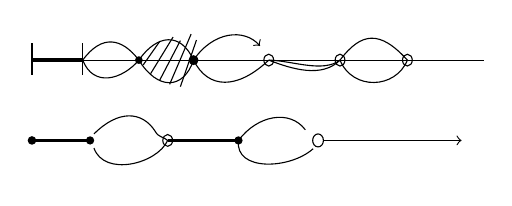
\begin{tikzpicture}[x=.62cm,y=.75cm]
\draw (0,0) -- (9.25,0);
\draw[line width=1.35pt] (0,0) -- (1.04,0);
\draw (0,-.25) -- (0,.29) (1.04,-.25) -- (1.04,.29);
\draw (1.04,0) .. controls (1.43,.44) and (1.84,.38) .. (2.19,0)
  .. controls (1.85,-.33) and (1.26,-.47) .. (1.04,0);
\draw (2.19,0) .. controls (2.56,.44) and (3.05,.48) .. (3.31,0)
  .. controls (3.10,-.51) and (2.57,-.51) .. (2.19,0);
\draw (2.28,-.08) -- (2.62,.32) (2.43,-.23) -- (2.89,.39)
      (2.61,-.35) -- (3.04,.33) (2.82,-.41) -- (3.26,.44)
      (3.04,-.45) -- (3.37,.34);
\fill (2.19,0) circle (1.4pt) (3.31,0) circle (1.8pt);
\draw[->] (3.31,0) .. controls (3.71,.49) and (4.35,.54) .. (4.67,.24);
\draw (3.31,0) .. controls (3.61,-.50) and (4.21,-.50) .. (4.85,0);
\draw (4.85,0) .. controls (5.32,-.15) and (5.94,-.31) .. (6.31,0);
\draw (4.85,0) .. controls (5.34,-.01) and (5.96,-.22) .. (6.31,0);
\draw (6.31,0) .. controls (6.75,.48) and (7.13,.51) .. (7.69,0)
  .. controls (7.45,-.49) and (6.57,-.52) .. (6.31,0);
\foreach \x in {4.85,6.31,7.69}
  \draw (\x,0) circle (.10);
\begin{scope}[yshift=-1.02cm]
\draw[line width=1.2pt] (0,0) -- (1.19,0) (2.78,0) -- (4.23,0);
\fill (0,0) circle (1.55pt) (1.19,0) circle (1.5pt) (4.23,0) circle (1.5pt);
\draw (1.27,.11) .. controls (1.78,.53) and (2.26,.49) .. (2.52,.16)
  .. controls (2.60,.04) and (2.69,.07) .. (2.78,0)
  .. controls (2.56,-.40) and (1.48,-.62) .. (1.27,-.13);
\draw (4.23,0) .. controls (4.62,.43) and (5.28,.53) .. (5.60,.18);
\draw (4.23,0) .. controls (4.15,-.53) and (5.29,-.49) .. (5.76,-.14);
\draw (2.78,0) circle (.10) (5.86,0) circle (.11);
\draw[->] (5.97,0) -- (8.80,0);
\end{scope}
\end{tikzpicture}}\endgroup}
\end{GelfandAdjacentEvidence}
\begin{GelfandAdjacentEvidence}{GELFAND-P000558}{7}


\uuline{В лакуну проектируется овал}: на каждом из них расп. по полюсу. Расп. полюсов зависит от нормировки: \(x_0\).

\sout{На одном листе […] , а на другом […]}
\Unclear{GELFAND-P000558}{ovals-fragment}{Начало зачёркнутой строки предположительно читается «На одном листе».}
\end{GelfandAdjacentEvidence}
\begin{GelfandAdjacentEvidence}{GELFAND-P000558}{8}

\Incomplete{GELFAND-P000558}{ovals-old}{После «листе» читаются отдельные штрихи. Далее, предположительно, «а на другом». Полное чтение не установлено.}
\end{GelfandAdjacentEvidence}

На каждом овале и по нулю.
\hfill\rule{1.4cm}{.35pt}\enspace\(\cdot\)\enspace\rule{1.4cm}{.35pt}\par
\uline{След. раз \mbox{$18^{\underline{30}}$}}


\Needspace{7\baselineskip}
\begin{GelfandAdjacentEvidence}{GELFAND-P000559}{1}
\SourcePage{GELFAND-P000559}{unlabelled}
\noindent\uwave{16.9.74.}\qquad\underline{Сем. Гельфанда.}\qquad\underline{Дубровин.}
\Unclear{GELFAND-P000559}{date-overwrite}{Второй знак даты переписан плотной петлёй. Текущее чтение «6» предположительно, прежний знак не читается.}
\end{GelfandAdjacentEvidence}
\begin{GelfandAdjacentEvidence}{GELFAND-P000559}{2}

\[
\text{Пусть}\quad L=-\frac{d^2}{dx^2}+u(x),\qquad u(x+T)=u(x).
\]
Спектр \(L\) — набор отрезков. Если их конечн. число, то он [вписано сверху: наз.] \uwave{конечнозонный}.
\Unclear{GELFAND-P000559}{finite-zone-ending}{В конце слова густо зачёркнута буква. Верхняя вставка предположительно «й», прежнее окончание не читается.}
\end{GelfandAdjacentEvidence}

Спектр — те \(\lambda\), для к-рых есть огр. решение ур-я \underline{\(Ly=\lambda y\)}.
\begin{gather*}
y_1(x+T)=\alpha_{11}y_1(x)+\alpha_{12}y_2(x)\\
y_2(x+T)=\alpha_{21}y_1(x)+\alpha_{22}y_2(x).
\end{gather*}
Матрица \((\alpha_{ij})=\widehat T\) (монодромии).

Надо, чтобы \(\widehat T^ny\) было ограничено, т. е. \(\exists\) соб. знач. с \(|\lambda|=1\)

но: \(\det\widehat T=1\) (Вронского); \(\lambda_1\lambda_2=1\).
\[
\begingroup\color{black}\GelfandFitDiagram{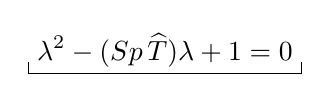
\begin{tikzpicture}[baseline=(eq.base)]
\node[inner xsep=3pt,inner ysep=2pt] (eq) {$\displaystyle
\lambda^2-(Sp\,\widehat T)\lambda+1=0$};
\draw ([yshift=4pt]eq.south west) -- (eq.south west) -- (eq.south east)
      -- ([yshift=4pt]eq.south east);
\end{tikzpicture}}\endgroup
\]


\Needspace{7\baselineskip}
\begin{GelfandAdjacentEvidence}{GELFAND-P000560}{1}
\SourcePage{GELFAND-P000560}{unlabelled}
\sout{Корни}
\Unclear{GELFAND-P000560}{top-old}{Зачёркнутое слово предположительно «Корни». Пересекающие штрихи скрывают часть букв.}
\end{GelfandAdjacentEvidence}
\begin{GelfandAdjacentEvidence}{GELFAND-P000560}{2}

\begin{gather*}
|\alpha_{11}+\alpha_{22}|<2\quad\Rightarrow\quad\text{корни компл.}\\
|\alpha_{11}+\alpha_{22}|>2\quad\Rightarrow\quad\text{корни вещ.}
\end{gather*}
Корни бегут в одну сторону (можно доказать).

\underline{Физ. интерпрет.}: если огр. соб. ф-я, то част. пролетит, если нет, то \sout{не} \fbox{\strut застрянет}
\Unclear{GELFAND-P000560}{trapped-old}{Перед словом в рамке короткое зачёркнутое слово предположительно «не».}
\end{GelfandAdjacentEvidence}
\begin{GelfandAdjacentEvidence}{GELFAND-P000560}{3}

\SourceFigure{GELFAND-P000560}{particle-wave}{%
\par\smallskip
\begingroup\color{black}\GelfandFitDiagram{\begin{tikzpicture}[x=.62cm,y=.65cm,every node/.style={inner sep=1pt}]
\draw (0,0) -- (4.62,0);
\fill (-.06,.57) circle (1.4pt);
\draw[->] (-.06,.57) -- (1.15,.61);
\draw (.02,.02) .. controls (.43,.68) and (.55,.49) .. (.68,.01)
  .. controls (1.02,-.97) and (1.40,.01) .. (1.64,.18)
  .. controls (1.81,.42) and (2.04,.37) .. (2.11,0)
  .. controls (2.34,-.94) and (2.70,.16) .. (2.99,.31)
  .. controls (3.24,.62) and (3.13,-.35) .. (3.40,-.43)
  .. controls (3.58,-.46) and (3.78,.59) .. (4.01,.42)
  .. controls (4.15,.31) and (4.05,-.06) .. (4.42,0);
\foreach \xa/\xb in {6.03/6.93,7.57/8.47,9.26/10.19} {
  \draw (\xa,0) -- (\xb,0);
  \draw (\xa,-.15) -- (\xa,.15) (\xb,-.15) -- (\xb,.15);
}
\draw (6.03,0) .. controls (6.28,.27) and (6.78,.31) .. (6.81,0);
\draw (7.57,0) .. controls (7.83,.31) and (8.46,.35) .. (8.47,0);
\draw (9.26,0) .. controls (9.56,.36) and (9.77,.21) .. (10.19,0);
\draw[->] (7.18,-.60) -- (7.31,-.16);
\draw[->] (8.43,-.75) -- (8.90,-.15);
\node[below,align=center] at (7.85,-.67) {\underline{запрещ.}\\\underline{зоны}};
\end{tikzpicture}}\endgroup\par}
\end{GelfandAdjacentEvidence}
\begin{GelfandAdjacentEvidence}{GELFAND-P000560}{4}

\uwave{exp убывают запр. зоны}. \hfill (резонанс част. и поля)\par
\Unclear{GELFAND-P000560}{decay-old}{В начале «убывают» видна верхняя черта над переписанными штрихами. Старое написание не читается.}
\end{GelfandAdjacentEvidence}
\begin{GelfandAdjacentEvidence}{GELFAND-P000560}{5}

\uwave{Айнс, Ахиезер, Хохштадт}.
\[
\text{\uwave{Ф-я Блоха}}\;-\;
\boxed{u(x+T)=\nu u(x)},\qquad |\nu|=1.\quad
(\text{соб. вектор }\widehat T).
\]
\[
\nu=e^{ip},\qquad p\text{ — «квазиимпульс»}.
\]
Огранич. соб. ф-и — если \(p\in\mathbb R\).
\SourceFigure{GELFAND-P000560}{band-lines}{%
\par\smallskip
\begingroup\color{black}\GelfandFitDiagram{\begin{tikzpicture}[x=.71cm,y=.72cm,every node/.style={inner sep=1pt}]
\draw (.22,0) -- (.60,0);
\draw[->] (1.21,0) -- (4.48,0);
\foreach \x in {.22,.60,1.21}
  \draw (\x,-.12) -- (\x,.12);
\node[anchor=west] at (5.59,.06) {\uwave{однозонный}};
\begin{scope}[yshift=-.63cm]
\draw (0,0) -- (.43,0) (.86,0) -- (1.65,0) (2.08,0) -- (2.85,0)
      (3.26,0) -- (4.07,0) (4.63,0) -- (6.53,0);
\foreach \x in {0,.43,.86,1.65,2.08,2.85,3.26,4.07,4.63}
  \draw (\x,-.13) -- (\x,.13);
\node[below left,inner sep=1pt] at (.43,-.13) {$E_1$};
\node[below right,inner sep=1pt] at (.86,-.13) {$E_2$};
\node[below] at (4.00,-.13) {$E_{2N}$};
\node[below right] at (4.57,-.13) {$E_{2N+1}$};
\end{scope}
\end{tikzpicture}}\endgroup\par}
\end{GelfandAdjacentEvidence}
\begin{GelfandAdjacentEvidence}{GELFAND-P000560}{6}

\[
\Gamma_N\text{ — риманова поверхность }\sqrt{R(E)},\qquad
\text{где}\quad R(E)=\prod_1^{2N+1}(E-E_i)
\]
\uuline{Г}. Пусть \(y(x,E)\) — блоховская ф-я для компл. \(E\).
\[
y(x+T)=\nu y(x)
\]
\(y(x_0,x,E)\)\qquad нормировка: \underline{\(y(x_0,x_0,E)=1\)}.
\SourceFigure{GELFAND-P000560}{complex-loop}{%
\par\smallskip
\begingroup\color{black}\GelfandFitDiagram{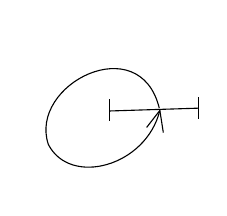
\begin{tikzpicture}[x=.73cm,y=.72cm]
\draw (.99,.04) -- (2.54,.09);
\draw (.99,-.13) -- (.99,.25) (2.54,-.10) -- (2.54,.29);
\draw (1.86,.09) .. controls (1.52,1.50) and (-.42,.51) .. (-.07,-.55)
  .. controls (.31,-1.30) and (1.63,-.94) .. (1.87,.05);
\draw (1.64,-.25) -- (1.87,.05) -- (1.93,-.34);
\end{tikzpicture}}\endgroup\par
У места встречи петли с отрезком два коротких расходящихся штриха. Направление отметки предположительно вверх.}
\end{GelfandAdjacentEvidence}
\begin{GelfandAdjacentEvidence}{GELFAND-P000560}{7}


\uuline{Д}.\quad\uuline{Т.~1.} Блоховские соб. ф-и аналит. прод. на \(\Gamma_N\).

\uuline{Т.~0}. Любой кон.-зонн. потенц. — стац. реш. высш. ур-я КДФ.

\uuline{Т.~2} Мн-во потенц. с зад. спектром — это \(J(\Gamma_N)\) — мн-зие Якоби.
\Unclear{GELFAND-P000560}{manifold-overwrite}{В «Мн-во» буква «в» переписана. Прежние штрихи не читаются.}
\end{GelfandAdjacentEvidence}
\begin{GelfandAdjacentEvidence}{GELFAND-P000560}{8}

Там действуют КДФ (дин. сист.) и его высш. аналоги.

В реш. \uwave{\mbox{$Ly=Ey$}} действует \((\widehat Ty)(x)=y(x+T)\)
\[
\begin{aligned}
c&=1,\quad c'=0\\
s&=0,\quad s'=1
\end{aligned}
\qquad(\text{в т. }x_0)\qquad c(x,x_0,E)
\]
В этом базисе матр. монодромии \underline{\(\alpha_{ij}(E,x_0)\)}.

Всё опр. следом матр. \(\tau=\frac12 Sp\,\alpha_{ij}\)
\[
|\tau|\le1\quad\Rightarrow\quad\text{зоны \underline{спектра}}
\]
\Unclear{GELFAND-P000560}{band-word}{Окончание «зоны» переписано. Прежние штрихи не читаются.}
\end{GelfandAdjacentEvidence}
\begin{GelfandAdjacentEvidence}{GELFAND-P000560}{9}

\[
\tau\text{ не зав. от }x_0,\qquad \underline{\tau=\tau(E)}.
\]
\[
\begingroup\color{black}\GelfandFitDiagram{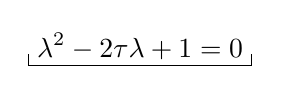
\begin{tikzpicture}[baseline=(eq.base)]
\node[inner xsep=3pt,inner ysep=2pt] (eq)
  {$\displaystyle\lambda^2-2\tau\lambda+1=0$};
\draw ([yshift=4pt]eq.south west) -- (eq.south west) -- (eq.south east)
      -- ([yshift=4pt]eq.south east);
\end{tikzpicture}}\endgroup
\]
\SourceFigure{GELFAND-P000560}{trace-graph}{%
\par\smallskip
\begingroup\color{black}\GelfandFitDiagram{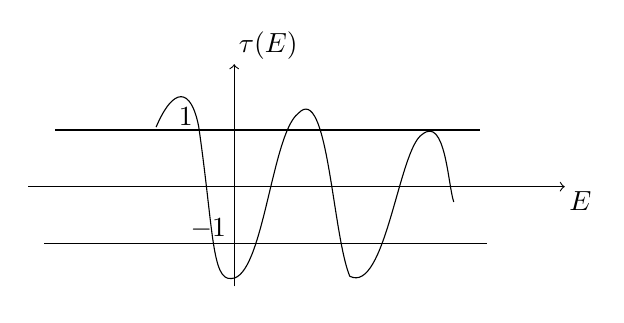
\begin{tikzpicture}[x=.82cm,y=.72cm,every node/.style={inner sep=1.5pt}]
\draw[->] (-3.19,0) -- (5.12,0) node[below right] {$E$};
\draw[->] (0,-1.76) -- (0,2.16) node[above right] {$\tau(E)$};
\draw (-2.77,1) -- (3.81,1);
\draw (-2.94,-1) -- (3.91,-1);
\node[above] at (-.75,1) {$1$};
\node[above] at (-.40,-1) {$-1$};
\draw (-1.21,1.05) .. controls (-.94,1.77) and (-.67,1.76) .. (-.55,1.06)
  .. controls (-.32,-.75) and (-.35,-1.67) .. (-.04,-1.62)
  .. controls (.45,-1.60) and (.58,.93) .. (.99,1.29)
  .. controls (1.45,1.86) and (1.52,-.84) .. (1.79,-1.58)
  .. controls (2.34,-1.90) and (2.55,.66) .. (2.91,.92)
  .. controls (3.27,1.26) and (3.31,.04) .. (3.40,-.27);
\end{tikzpicture}}\endgroup\par}
\end{GelfandAdjacentEvidence}
\begin{GelfandAdjacentEvidence}{GELFAND-P000560}{10}

изв., что график такой — \uwave{\mbox{$max$} и \mbox{$min\geqslant1$}} — \uwave{зад.}
\Unclear{GELFAND-P000560}{extrema-boundary}{Знак перед \(1\) состоит из верхней и двух косых черт. Предположительное чтение \(\geqslant\).}
\end{GelfandAdjacentEvidence}



\Needspace{7\baselineskip}
\begin{GelfandAdjacentEvidence}{GELFAND-P000561}{1}
\SourcePage{GELFAND-P000561}{unlabelled}
\uwave{для \mbox{$2^{*}$} курса} \quad Их всегда беск. число (\underline{\(max\) и \(min\)}).
\Unclear{GELFAND-P000561}{course-ordinal}{После «2» стоит малый перекрещенный знак. Сохранено начертание, чтение окончания не установлено.}
\end{GelfandAdjacentEvidence}
\begin{GelfandAdjacentEvidence}{GELFAND-P000561}{2}

слияние 2-х запр. зон — нет разр. зоны
\SourceFigure{GELFAND-P000561}{touching-maxima}{%
\par\smallskip
\begingroup\color{black}\GelfandFitDiagram{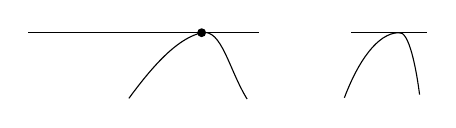
\begin{tikzpicture}[x=.77cm,y=.81cm]
\draw (0,0) -- (3.80,0);
\draw (1.66,-1.03) .. controls (2.16,-.38) and (2.52,-.08) .. (2.86,0)
  .. controls (3.19,.07) and (3.31,-.58) .. (3.61,-1.04);
\fill (2.86,0) circle (1.6pt);
\begin{scope}[xshift=4.1cm]
\draw (0,0) -- (1.26,0);
\draw (-.11,-1.02) .. controls (.12,-.44) and (.44,-.01) .. (.78,0)
  .. controls (.96,.05) and (1.08,-.60) .. (1.13,-.97);
\end{scope}
\end{tikzpicture}}\endgroup\par}
\end{GelfandAdjacentEvidence}
\begin{GelfandAdjacentEvidence}{GELFAND-P000561}{3}

У ур-я \underline{\(\tau(E)=\pm1\)} надо отобрать \uuline{простые} корни для опр. концов зон.

\underline{Концы зон} \uwave{дают жорд. клетку}. Если диагон., то получ. вырожд. случай.

См. раб. \uuline{Гельфанда и Лидского} (1955) о системах с периодич. коэфф..

\uuline{Опр.}\quad
\(\Psi(x,x_0,E),\qquad \Psi(x+T)=e^{ip}\Psi(x),\qquad \Psi(x_0)=1.\)

Другая компл. сопряжена (при \(|\tau(E)|<1\)).
\[
\text{Пусть}\qquad
\begingroup\color{black}\GelfandFitDiagram{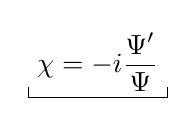
\begin{tikzpicture}[baseline=(eq.base)]
\node[inner xsep=3pt,inner ysep=2pt] (eq)
  {$\displaystyle\chi=-i\frac{\Psi'}{\Psi}$};
\draw ([yshift=4pt]eq.south west) -- (eq.south west) -- (eq.south east)
      -- ([yshift=4pt]eq.south east);
\end{tikzpicture}}\endgroup
\]
1.\quad \(\chi=\chi(x,E)\qquad(\text{не зав. от }x_0)\).
\Unclear{GELFAND-P000561}{detached-mark}{Справа между первой и второй строками списка стоит отдельное «, и». Его привязка неясна.}
\end{GelfandAdjacentEvidence}
\begin{GelfandAdjacentEvidence}{GELFAND-P000561}{4}

2.\quad
\begingroup\color{black}\GelfandFitDiagram{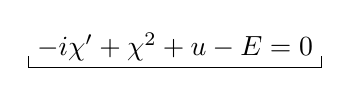
\begin{tikzpicture}[baseline=(eq.base)]
\node[inner xsep=3pt,inner ysep=2pt] (eq) {$-i\chi'+\chi^2+u-E=0$};
\draw ([yshift=4pt]eq.south west) -- (eq.south west) -- (eq.south east)
      -- ([yshift=4pt]eq.south east);
\end{tikzpicture}}\endgroup
\qquad (ур-е Риккати).
\[
3.\quad \chi_I=\frac12\frac{\chi_R'}{\chi_R},\qquad
\uwave{\mbox{$\chi=\chi_R+i\chi_I.$}}
\]
\[
4.\quad \chi(x,E)\sim k+\sum_{n=1}^{\infty}\frac{\chi_n(x)}{(2k)^n},
\qquad \text{где } k=\sqrt E
\]
\Unclear{GELFAND-P000561}{series-asymptotic-overwrite}{Перед \(k\) видна волна поверх старых штрихов. Чтение \(\sim\) предположительно.}
\end{GelfandAdjacentEvidence}
\begin{GelfandAdjacentEvidence}{GELFAND-P000561}{5}

5.\quad \(\chi(x+T)=\chi(x)\). (асимпт. разложение).
\[
\uwave{\mbox{$2\Rightarrow3$}},\qquad 2\Rightarrow4
\]
\Incomplete{GELFAND-P000561}{implication-old}{После \(2\Rightarrow4\) густо зачёркнута группа знаков. Сохранившихся штрихов недостаточно для чтения.}
\end{GelfandAdjacentEvidence}
\begin{GelfandAdjacentEvidence}{GELFAND-P000561}{6}

\Unclear{GELFAND-P000561}{odd-series-prefix}{Перед \(\chi_R\) зачёркнута короткая группа. Предположительно \(\chi\) с индексом, возможно \(R\).}
\end{GelfandAdjacentEvidence}
\begin{GelfandAdjacentEvidence}{GELFAND-P000561}{7}

\[
\chi_R(x,E)=k+\sum_{n=0}^{\infty}\frac{\chi_{2n+1}(x)}{(2k)^{2n+1}}
\]
\[
\Psi=\exp\left(i\int_{x_0}^{x}\chi\,dx\right)
=\sqrt{\frac{\chi_R(x_0)}{\chi_R(x)}}\exp\left(i\int_{x_0}^{x}\chi_R\,dx\right).
\]
\[
1.\quad|\Psi|^2=\frac{\chi_R(x_0)}{\chi_R(x)}
\]
\[
2.\quad p(E)=\int_0^T\chi_R(x,E)\,dx+\pi n
\]
\Unclear{GELFAND-P000561}{phase-addend}{Перед \(\pi n\) густой наклонный знак. Чтение отдельного множителя не установлено.}
\end{GelfandAdjacentEvidence}
\begin{GelfandAdjacentEvidence}{GELFAND-P000561}{8}

Выразим \(\chi\) через матр. монодромии.

\sout{\underline{Теор.}}\quad\underline{Лемма}
\Unclear{GELFAND-P000561}{lemma-cancel}{Подчёркнутое «Теор.» зачёркнуто. Справа и выше вписано «Лемма».}
\end{GelfandAdjacentEvidence}
\begin{GelfandAdjacentEvidence}{GELFAND-P000561}{9}

\begin{equation*}
\chi(x,E)=\frac{\sqrt{1-\tau^2(E)}}{\alpha_{21}(E,x)}
+\frac i2\frac{\alpha_{11}(E,x)\alpha_{22}(E,x)}{\alpha_{21}(E,x)}
\tag{1}
\end{equation*}
\Unclear{GELFAND-P000561}{monodromy-numerator}{Между \(\alpha_{11}(E,x)\) и \(\alpha_{22}(E,x)\) отдельный знак не различим. Группы переданы рядом.}
\end{GelfandAdjacentEvidence}

\underline{Д-во.}\quad \(\Psi(x,x_0,E)\) — соб. вектор матр. монодр. Ищем по прав. лин. алгебры:
\[
\Psi(x,x_0,E)=c(x,x_0,E)+
i\left(\begin{gathered}\text{прав. часть}\\\text{ф-лы (1) в т. }x_0\end{gathered}\right)s(x,x_0,E).
\]


\Needspace{7\baselineskip}
\begin{GelfandAdjacentEvidence}{GELFAND-P000562}{1}
\SourcePage{GELFAND-P000562}{unlabelled}
Найдём опр. Вронского этой ф-и и \(c\) (он не зав. от \(x\)).
\begin{gather*}
\left.\{c,\Psi(x,x_0,E)\}\right|_{x_0}=\qquad\text{всё получается.}\\
i\chi(x_0,E)=i(\ldots)\\
\left.\{c,\Psi\}\right|_{x_0}=i\Psi'(x_0)=i\chi(x_0).
\end{gather*}
\Unclear{GELFAND-P000562}{wronskian-overwrite}{После \(i\) стоит переписанный знак со штрихом. Текущее чтение \(\Psi'\) предположительно.}
\end{GelfandAdjacentEvidence}
\begin{GelfandAdjacentEvidence}{GELFAND-P000562}{2}

\SourceFigure{GELFAND-P000562}{degenerate-trace}{%
\par\smallskip
\begingroup\color{black}\GelfandFitDiagram{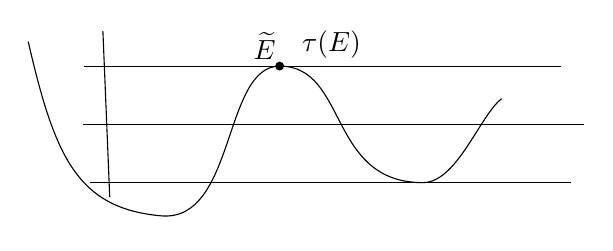
\begin{tikzpicture}[x=.87cm,y=.74cm,every node/.style={inner sep=1pt}]
\draw (-2.18,1) -- (4.78,1) (-2.20,0) -- (5.12,0)
      (-2.10,-1) -- (4.92,-1);
\draw (-1.91,1.60) -- (-1.81,-1.25);
\draw (-3.00,1.42) .. controls (-2.61,-.57) and (-2.28,-1.44) .. (-1.06,-1.57)
  .. controls (.03,-1.68) and (-.16,1) .. (.67,1)
  .. controls (1.67,1) and (1.37,-1) .. (2.76,-1)
  .. controls (3.26,-1) and (3.59,.15) .. (3.91,.44);
\fill (.67,1) circle (1.6pt);
\node[above left] at (.66,1.05) {$\widetilde E$};
\node[above right] at (.95,1.08) {$\tau(E)$};
\end{tikzpicture}}\endgroup\par}
\end{GelfandAdjacentEvidence}
\begin{GelfandAdjacentEvidence}{GELFAND-P000562}{3}

Если \((1-\tau(E))\) им. кратный 0, то матр. монодромии диагональна, т. е.
\Unclear{GELFAND-P000562}{diagonal-prefix-old}{Перед равенствами зачёркнут короткий знак, похожий на «π». Его чтение не установлено.}
\end{GelfandAdjacentEvidence}
\begin{GelfandAdjacentEvidence}{GELFAND-P000562}{4}

\[
\uwave{\mbox{$\alpha_{12}(\widetilde E,x_0)=0,\qquad
             \alpha_{21}(\widetilde E,x_0)=0.$}}
\]
\[
\frac{1-\tau^2(E)}{R(E)}\quad\text{\uwave{имеет лишь 2-кр. вырожд. нули}.}
\]
\Unclear{GELFAND-P000562}{quotient-old}{Слева и сверху дроби густо зачёркнуты косая черта и верхняя линия. Возможно, снят знак корня.}
\end{GelfandAdjacentEvidence}
\begin{GelfandAdjacentEvidence}{GELFAND-P000562}{5}

\[
\sqrt{\frac{1-\tau^2(E)}{R(E)}}\quad
\text{\uwave{имеет лишь простые нули}.}\qquad(\text{см. Титчмарш})
\]
\underline{\(\alpha_{21}(\widetilde E,x_0)=0\)} \underline{тоже}
\[
\uwave{\mbox{$\displaystyle\alpha_{21}=\widetilde\alpha_{21}\cdot
\sqrt{\frac{1-\tau^2(E)}{R(E)}}$}}\qquad(\text{поделили}).
\]
Подставим в ф-лу \(\chi_R\):
\[
\chi_R=\frac{\sqrt{R(E)}}{\widetilde\alpha_{21}(E,x)},
\qquad\text{где }\widetilde\alpha_{21}(E,x)\text{ — целая анал. ф-я от }E.
\]
\[
\chi_R=k+O\left(\frac1k\right),\qquad
\sqrt{R(E)}\sim E^N\quad\text{на бесконечн.}.
\]
\Unclear{GELFAND-P000562}{infinity-power}{Видимая степень в этой строке \(N\). В следующей строке в числителе стоит \(kE^N\).}
\end{GelfandAdjacentEvidence}
\begin{GelfandAdjacentEvidence}{GELFAND-P000562}{6}

\[
\chi_R(x,E)\sim\frac{kE^N}{E^N}\quad\Rightarrow\quad
\widetilde\alpha_{21}(E,x)\text{ — полином по }E.
\]
\hfill\uwave{\mbox{$P(E,x)$}}\par
\(\chi_R(x,E)\) — 2-значн. аналит. ф-я (аналит. прод. из вещ. \(E\) в зоне)
\[
\chi_R(x,E)=\frac{\sqrt{R(E)}}{P(E,x)}
\]
\[
P(E,x)=\prod(E-\gamma_i(x)),\qquad
\gamma_i(x)\text{ — корни многочлена}
\]
\[
\text{Отсюда}:\quad
\boxed{\chi(x,E)=\left(\sqrt R-\frac i2\frac d{dx}P\right)/P.}
\]
\[
\chi_R\sim k+\sum\frac{\chi_{2n+1}(x)}{(2k)^{2n+1}}
\]
\Unclear{GELFAND-P000562}{odd-index}{В индексе \(2n+1\) буква \(n\) переписана. Прежние штрихи не читаются.}
\end{GelfandAdjacentEvidence}

Построим ф-лы
\[
I_n\{u\}=\int_0^T\chi_{2n+3}(x)\,dx
\]


\Needspace{7\baselineskip}
\begin{GelfandAdjacentEvidence}{GELFAND-P000563}{1}
\SourcePage{GELFAND-P000563}{unlabelled}
\[
\begingroup\color{black}\GelfandFitDiagram{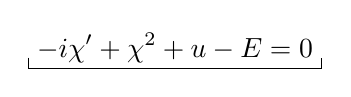
\begin{tikzpicture}[baseline=(eq.base)]
\node[inner xsep=3pt,inner ysep=2pt] (eq) {$\displaystyle-i\chi'+\chi^2+u-E=0$};
\draw ([yshift=4pt]eq.south west) -- (eq.south west) -- (eq.south east)
      -- ([yshift=4pt]eq.south east);
\end{tikzpicture}}\endgroup
\quad\Rightarrow\quad\text{асимптотика}.
\]
и при этом \(\chi_{2n+1}=Q(u,u',\ldots,u^{(n-1)})\) — \uwave{многочлен}.
\Unclear{GELFAND-P000563}{derivative-order}{Показатель у последнего \(u\) читается предположительно как \((n-1)\).}
\end{GelfandAdjacentEvidence}
\begin{GelfandAdjacentEvidence}{GELFAND-P000563}{2}

\Unclear{GELFAND-P000563}{left-old-symbol}{Слева зачёркнута группа с вертикальными чертами и петлёй. Видимый знак похож на «δ» или «\(\int\)», прежняя запись не установлена.}
\end{GelfandAdjacentEvidence}
\begin{GelfandAdjacentEvidence}{GELFAND-P000563}{3}

\sout{Это […]}
\Unclear{GELFAND-P000563}{stationary-fragment}{Начало зачёркнутой строки предположительно «Это».}
\end{GelfandAdjacentEvidence}
\begin{GelfandAdjacentEvidence}{GELFAND-P000563}{4}

\Incomplete{GELFAND-P000563}{stationary-old}{Оставшиеся слова в зачёркнутой строке не читаются.}
\end{GelfandAdjacentEvidence}

\[
\frac{\delta}{\delta u}\left\{\sum c_n I_n\right\}=d\quad(=const).
\]
\noindent\(\cdot\quad\cdot\quad\cdot\quad\cdot\quad\cdot\quad\cdot\quad\cdot
\quad\cdot\quad\cdot\quad\cdot\quad\cdot\quad\cdot\quad\cdot\)


\Needspace{7\baselineskip}
\begin{GelfandAdjacentEvidence}{GELFAND-P000564}{1}
\SourcePage{GELFAND-P000564}{unlabelled}
\noindent\hfill\rule{1.35cm}{.28pt}\enspace\rule{.55cm}{.40pt}\hfill\mbox{}\par
\uwave{\mbox{$23/\underline{\overline{\mathrm{IX}}}-74$}}\qquad\uuline{Сем. Гельфанда.}

О раб. \uwave{Габриэлова, И. Гельфанда и Лосика} по комбинаторной топологии.

Интересно сделать аналитически.
\sout{\mbox{$\int$} […]}
\Unclear{GELFAND-P000564}{analytic-fragment}{В начале зачёркнутой группы виден знак с двумя петлями, предположительно \(\int\).}
\end{GelfandAdjacentEvidence}
\begin{GelfandAdjacentEvidence}{GELFAND-P000564}{2}

\Incomplete{GELFAND-P000564}{analytic-old}{Остальные знаки перекрыты косыми чертами и не читаются.}
\end{GelfandAdjacentEvidence}
\begin{GelfandAdjacentEvidence}{GELFAND-P000564}{3}

\[
\int_{1-x}^{x}\left[\frac{\log|t|}{1-t}+\frac{\log|1-t|}{t}\right]\,dt
\]
не вычисл. в элем. ф-ях. Но:
\[
\int_0^1\frac{\log|1-t|}{t}\,dt=\frac{\pi^2}{6}
\quad\left(=\int_0^1\sum_{n=1}^{\infty}\frac{t^{n-1}}n
=\sum_{n=1}^{\infty}\frac1{n^2}\right).
\]
\Unclear{GELFAND-P000564}{integral-sign}{Перед \(\pi^2/6\) знака минус нет. В среднем члене дифференциал не написан.}
\end{GelfandAdjacentEvidence}
\begin{GelfandAdjacentEvidence}{GELFAND-P000564}{4}

Можно вычислить
\[
\int_{2-\sqrt5}^{\sqrt5-2}\left[\frac{\log|t|}{1-t}+\frac{\log|1-t|}{t}\right]\,dt
=-\frac{\pi^2}{6}
\]
\Unclear{GELFAND-P000564}{symmetric-integral}{В этой строке перед \(\pi^2/6\) виден минус. Пределы \(2-\sqrt5\) и \(\sqrt5-2\).}
\end{GelfandAdjacentEvidence}
\begin{GelfandAdjacentEvidence}{GELFAND-P000564}{5}

(из топологических соображений).
\Unclear{GELFAND-P000564}{topological-overwrite}{В обоих словах есть переписанные буквы. Старые штрихи не читаются.}
\end{GelfandAdjacentEvidence}
\begin{GelfandAdjacentEvidence}{GELFAND-P000564}{6}

Они встречаются в конечной комбинаторной задаче.

\uwave{Грэм Сигаль} — всю топологию.

\uuline{Джусти.} Об особенностях. (On regularity of \sout{[…]} solv. of nonlin. syst.).
\Unclear{GELFAND-P000564}{speaker-name}{Имя читается предположительно как «Джусти». Средние штрихи слиты.}
\end{GelfandAdjacentEvidence}
\begin{GelfandAdjacentEvidence}{GELFAND-P000564}{7}

\Incomplete{GELFAND-P000564}{regularity-old}{В английской скобке перед «solv.» густо зачёркнута короткая запись. Она не читается.}
\end{GelfandAdjacentEvidence}
\begin{GelfandAdjacentEvidence}{GELFAND-P000564}{8}

\uwave{Symplest case}:
\[
\sum_{i,j=1}^{n}\sum_{h,k=1}^{N}\int a_{ij}^{hk}(x,u)D_i u^h D_j\varphi^k\,dx=0
\]
\Unclear{GELFAND-P000564}{weak-overwrites}{В аргументе \((x,u)\) и перед верхним \(k\) есть переписанные знаки. Текущие чтения \(u\) и \(\varphi\) предположительны.}
\end{GelfandAdjacentEvidence}
\begin{GelfandAdjacentEvidence}{GELFAND-P000564}{9}

\[
D_i=\frac\partial{\partial x},\qquad
\forall\varphi=(\varphi^1,\ldots,\varphi^N),\qquad
\varphi_i\in W_0^{1,2}(\Omega)
\]
\Unclear{GELFAND-P000564}{test-component-old}{Под \(\varphi^1\) густой нижний знак. Возможны \(2\), \(i\) или \(z\), чтение не установлено.}
\end{GelfandAdjacentEvidence}
\begin{GelfandAdjacentEvidence}{GELFAND-P000564}{10}

\[
\sum_{i,j=1}^{n}\sum_{h=1}^{N}D_j\bigl(a_{ij}^{hk}(x,u)D_i u^k\bigr)=0
\qquad(k=1,2,\ldots,N)
\]
\Unclear{GELFAND-P000564}{system-indices}{В знаменателе \(D_i\) написано \(\partial x\). В сумме по \(h\) справа видна степень \(k\) у \(u\).}
\end{GelfandAdjacentEvidence}
\begin{GelfandAdjacentEvidence}{GELFAND-P000564}{11}

\[
u=(u^1,\ldots,u^N).
\]
\uwave{Ellipticity}:
\[
\sum_{ijhk}a_{ij}^{hk}(x,t)\xi_i^h\xi_j^k\geqslant|\xi|^2,\qquad
\forall x\in\Omega,\ \forall t\in\mathbb R^n
\]
\Unclear{GELFAND-P000564}{ellipticity-indices}{Первый нижний индекс у \(\xi\) предположительно \(i\). Последняя размерность читается как \(n\).}
\end{GelfandAdjacentEvidence}



\Needspace{7\baselineskip}
\begin{GelfandAdjacentEvidence}{GELFAND-P000565}{1}
\SourcePage{GELFAND-P000565}{unlabelled}
\[
\sum_{i,j=1}^{n}D_j\bigl(A_{ij}(x,u)D_i u\bigr)=0,
\qquad\begin{gathered}
u\text{ — вектор}\\
A_{ij}\text{ — матрица}.
\end{gathered}
\]
\underline{\(N=1\)} \(\ \Rightarrow\forall\) solution is regular

or \underline{\(n\leqslant2\)}\qquad
\(\forall u\in W^{1,1}\) is regular (depende on reg. of \(A\)-coefficients)
\Unclear{GELFAND-P000565}{dimension-overwrite}{Знак между \(n\) и \(2\) переписан. Текущее чтение \(\leqslant\) предположительно.}
\end{GelfandAdjacentEvidence}
\begin{GelfandAdjacentEvidence}{GELFAND-P000565}{2}

\Unclear{GELFAND-P000565}{coefficient-old}{Знак перед «coefficients» переписан, предположительно «A». Старые штрихи не читаются.}
\end{GelfandAdjacentEvidence}
\begin{GelfandAdjacentEvidence}{GELFAND-P000565}{3}

\[
A\in C^\infty\quad\Rightarrow\quad u\in C^\infty\quad\text{etc.}
\]
\begin{gather*}
W^{1,2},\qquad u\in L_2,\qquad \int_{\Omega}|Du|^2\,dx<+\infty\\
W_0^{1,2}\text{ — 0 boundary values.}
\end{gather*}
\Unclear{GELFAND-P000565}{boundary-overwrite}{В «boundary» буква «d» переписана. Над словом стоит \(\Omega\) под интегралом предыдущей строки.}
\end{GelfandAdjacentEvidence}
\begin{GelfandAdjacentEvidence}{GELFAND-P000565}{4}

\(n=\)\underline{\(N\geqslant3\)}\qquad\uwave{falls}.
\Unclear{GELFAND-P000565}{dimension-three}{Цифра «3» переписана. Под ней видны старые штрихи, чтение которых не установлено.}
\end{GelfandAdjacentEvidence}
\begin{GelfandAdjacentEvidence}{GELFAND-P000565}{5}

\Unclear{GELFAND-P000565}{fails-spelling}{В английском слове видны две высокие петли без точки над первой. Передано «falls».}
\end{GelfandAdjacentEvidence}
\begin{GelfandAdjacentEvidence}{GELFAND-P000565}{6}

\[
a_{ij}^{hk}=\delta_{ij}\delta_{hk}+
\left(\delta_{jk}+\frac1{n-2}\frac{u_j u_k}{1+|u|^2}\right)
\left(\delta_{ih}+\frac4{n-2}\frac{u_i u_h}{1+|u|^2}\right)
\]
\Unclear{GELFAND-P000565}{coefficient-formula}{Перед дробями в двух скобках различимы множители \(1/(n-2)\) и \(4/(n-2)\) в этом порядке.}
\end{GelfandAdjacentEvidence}
\begin{GelfandAdjacentEvidence}{GELFAND-P000565}{7}

\uwave{\mbox{$u_i=x_i/|x|$}} — \uwave{solution}.
\qquad\uwave{coefficients are real analityc}
\Unclear{GELFAND-P000565}{source-english-spelling}{Английское написание «analityc» сохранено.}
\end{GelfandAdjacentEvidence}
\begin{GelfandAdjacentEvidence}{GELFAND-P000565}{8}

\underline{\(n=2\)}\qquad \(\forall\) sol. is regular

\underline{\(n=3,\ N=2\)} — there is an example of non regular solution.

\uwave{For Dirichlet problem}. \(u_i=x_i\) when \(|x|=1\).
\(\exists!\) solution and it is not regular!

\noindent\hfill\rule{1.1cm}{.32pt}\enspace\(\cdot\)\enspace\rule{.9cm}{.32pt}\par
Suppose \(a_{ij}^{hk}\) are \uwave{continuous}

Then (1) \(\forall\) solution \(u\) of system is regular in an open set \(\Omega_0\subset\Omega\)
\Unclear{GELFAND-P000565}{old-number}{Перед «(2)» зачёркнута запись в скобках. Старый номер не читается.}
\end{GelfandAdjacentEvidence}
\begin{GelfandAdjacentEvidence}{GELFAND-P000565}{9}

(2). \(K=\Omega-\Omega_0\) (\(K\) is closed in \(\Omega\)) \sout{a[…]}
\[
\Rightarrow\underset{H_{n-2}}{\mathrm{meas}} K=0
\]
\Unclear{GELFAND-P000565}{old-at}{В зачёркнутом английском слове видно начальное «a». Остальные буквы не установлены.}
\end{GelfandAdjacentEvidence}
\begin{GelfandAdjacentEvidence}{GELFAND-P000565}{10}

\[
\uwave{\mbox{$\dim K<n-2.$}}
\]
\Unclear{GELFAND-P000565}{hausdorff-sign}{В строке с \(\dim K\) нижний штрих знака утолщён. По видимому контуру передано \(<\).}
\end{GelfandAdjacentEvidence}
\begin{GelfandAdjacentEvidence}{GELFAND-P000565}{11}

(for order \(m>2\qquad\dim K\leqslant n-2\)).

\noindent\hfill\rule{1.1cm}{.32pt}\enspace\(\cdot\)\enspace\rule{.9cm}{.32pt}\par
\sout{There} Are \sout{also} [вписано сверху] there variational problems with nonregular solutions?
\Unclear{GELFAND-P000565}{variational-old}{Перед «Are» зачёркнуто предположительно «There», после него — предположительно «also». Вписанное сверху «there» обведено.}
\end{GelfandAdjacentEvidence}

\noindent\hfill\rule{1.1cm}{.32pt}\enspace\(\cdot\)\enspace\rule{.9cm}{.32pt}\par
\uuline{Problem of Gelfand}. Придумать аналог разреш. особ. по Хиронаке для эллипт. ур-й.


\Needspace{7\baselineskip}
\begin{GelfandAdjacentEvidence}{GELFAND-P000566}{1}
\SourcePage{GELFAND-P000566}{unlabelled}
\uwave{И. М. Гельфанд}\qquad повторение прошлого докл. Дубровина.
\SourceFigure{GELFAND-P000566}{heading-capped-separator}{%
\par\smallskip
\begingroup\color{black}\GelfandFitDiagram{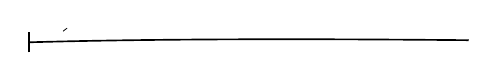
\begin{tikzpicture}[x=.75cm,y=.67cm]
\draw[line width=.6pt] (0,0) .. controls (2.5,.08) and (5.5,.06) .. (7.45,.04);
\draw[line width=.8pt] (0,-.19) -- (0,.20);
\draw[line width=.28pt] (.58,.21) -- (.65,.27);
\end{tikzpicture}}\endgroup\par
Над левым концом виден небольшой отдельный косой штрих.}
\end{GelfandAdjacentEvidence}
\begin{GelfandAdjacentEvidence}{GELFAND-P000566}{2}

\begin{gather*}
-y''+u(x)y=Ey\\
u(x+T)=u(y)
\end{gather*}
\Unclear{GELFAND-P000566}{period-argument}{Справа отчётливо читается \(u(y)\).}
\end{GelfandAdjacentEvidence}
\begin{GelfandAdjacentEvidence}{GELFAND-P000566}{3}

Спектр — те \(E\), при к-рых есть огранич. соб. ф-и.
\Unclear{GELFAND-P000566}{energy-overwrites}{Обе буквы \(E\) переписаны плотными штрихами. Прежние знаки не установлены.}
\end{GelfandAdjacentEvidence}
\begin{GelfandAdjacentEvidence}{GELFAND-P000566}{4}

\uwave{Проблема Новикова}: когда есть конечн. число запрещ. зон?
\SourceFigure{GELFAND-P000566}{spectral-bands}{%
\par\smallskip
\begingroup\color{black}\GelfandFitDiagram{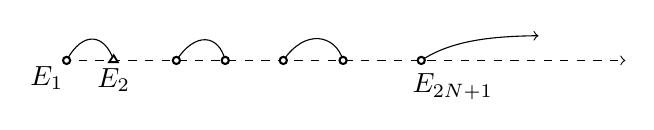
\begin{tikzpicture}[x=.73cm,y=.73cm,every node/.style={inner sep=1pt}]
\draw[dashed,->] (.32,0) -- (10.12,0);
\draw (.40,0) .. controls (.68,.52) and (1.06,.47) .. (1.22,0);
\draw (2.31,0) .. controls (2.64,.51) and (3.05,.45) .. (3.16,0);
\draw (4.17,0) .. controls (4.55,.56) and (5.08,.45) .. (5.21,0);
\draw[->] (6.57,0) .. controls (7.07,.33) and (7.72,.42) .. (8.61,.43);
\foreach \x in {.40,2.31,3.16,4.17,5.21,6.57}
  \draw[line width=.75pt,fill=white] (\x,0) circle (1.3pt);
\draw[line width=.65pt,fill=white] (1.14,-.03) -- (1.29,-.03) -- (1.22,.09) -- cycle;
\node[below left] at (.40,-.05) {$E_1$};
\node[below] at (1.22,-.09) {$E_2$};
\node[below right] at (6.36,-.18) {$E_{2N+1}$};
\end{tikzpicture}}\endgroup\par}
\end{GelfandAdjacentEvidence}
\begin{GelfandAdjacentEvidence}{GELFAND-P000566}{5}

\uuline{Т. Новик.-Дубров}.
\Unclear{GELFAND-P000566}{theorem-name}{В конце «Дубров.» густой переписанный штрих. Прежняя буква не установлена.}
\end{GelfandAdjacentEvidence}
\begin{GelfandAdjacentEvidence}{GELFAND-P000566}{6}

Это потенциалы \(\Leftrightarrow\) удовл. нелин. ур-ю
\[
K(u,u',\ldots,u^{(2N)})=0
\]
(Высш. ур-е Кортевега-де Фриса)
\begin{align*}
c(x,x_0,E)&:\qquad c(x_0)=1,\quad c'(x_0)=0\\
s(x,x_0,E)&:\qquad s(x_0)=0,\quad s'(x_0)=1.
\end{align*}
Это аналит. ф-и параметра \(E\).
\[
\widehat T\Psi=\Psi(x+T),\qquad
\widehat T=\begin{pmatrix}\alpha_{11}&\alpha_{12}\\
                           \alpha_{21}&\alpha_{22}\end{pmatrix}
\qquad\det\|\widehat T\|=1.
\]
Ф-я Блоха: \uwave{\mbox{$\Psi(x+T)=\lambda\Psi(x)$}},\qquad \(\Psi(x_0)=1\)

Это соб. вектор для \(\widehat T\).
\begin{gather*}
\lambda^2-(\alpha_{11}+\alpha_{22})\lambda+1=0,\\
\lambda^2-2\tau\lambda+1=0,\qquad
\tau(E)=\frac{\alpha_{11}+\alpha_{22}}2.
\end{gather*}
\(E\in\) допуст. интерв. \(\Leftrightarrow\exists\) Блох. ф-я с \(|\lambda|=1\).

\(\tau^2\leqslant1\) — разреш. инт., \(\tau^2>1\) — запрещ.
\SourceFigure{GELFAND-P000566}{first-trace}{%
\par\smallskip
\begingroup\color{black}\GelfandFitDiagram{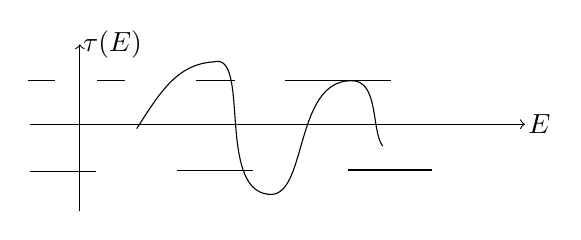
\begin{tikzpicture}[x=.84cm,y=.7cm,every node/.style={inner sep=1pt}]
\draw[->] (-.75,0) -- (6.73,0) node[right] {$E$};
\draw[->] (0,-1.58) -- (0,1.45) node[right] {$\tau(E)$};
\draw (-.78,.79)--(-.37,.79) (.26,.79)--(.68,.79)
      (1.75,.79)--(2.34,.79) (3.10,.79)--(4.70,.79);
\draw (-.75,-.86)--(.24,-.86) (1.47,-.84)--(2.62,-.84)
      (4.06,-.83)--(5.33,-.83);
\draw (.86,-.08) .. controls (1.20,.55) and (1.46,1.09) .. (2.02,1.13)
  .. controls (2.58,1.33) and (2.07,-1.16) .. (2.84,-1.27)
  .. controls (3.45,-1.39) and (3.22,.78) .. (4.10,.79)
  .. controls (4.53,.80) and (4.40,-.11) .. (4.58,-.40);
\end{tikzpicture}}\endgroup\par}
\end{GelfandAdjacentEvidence}
\begin{GelfandAdjacentEvidence}{GELFAND-P000566}{7}

все \(max\geqslant1\qquad\) (такой вид).

Правильный рис.:
\SourceFigure{GELFAND-P000566}{corrected-trace}{%
\par\smallskip
\begingroup\color{black}\GelfandFitDiagram{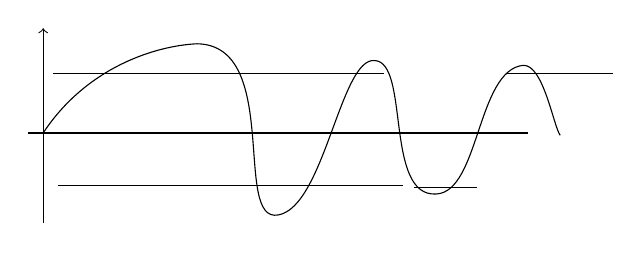
\begin{tikzpicture}[x=.76cm,y=.76cm]
\draw[->] (0,-1.50) -- (0,1.75);
\draw (-.25,0) -- (8.10,0);
\draw (.16,1)--(5.70,1) (7.75,1)--(9.53,1);
\draw (.25,-.88)--(6.02,-.88) (6.19,-.91)--(7.25,-.91);
\draw (0,0) .. controls (.74,1.12) and (1.91,1.46) .. (2.57,1.49)
  .. controls (3.99,1.47) and (3.16,-1.52) .. (3.93,-1.37)
  .. controls (4.70,-1.23) and (4.97,1.27) .. (5.54,1.21)
  .. controls (6.13,1.18) and (5.70,-1.08) .. (6.57,-1.02)
  .. controls (7.29,-.98) and (7.25,1.05) .. (8.02,1.13)
  .. controls (8.36,1.15) and (8.53,.10) .. (8.64,-.04);
\end{tikzpicture}}\endgroup\par}
\end{GelfandAdjacentEvidence}
\begin{GelfandAdjacentEvidence}{GELFAND-P000566}{8}

Запрещ. зоны сжимаются.

\uline{Важный вывод}: если все зоны слились, то, \(max\) и \(min\) начин. с нек-ро равны \(1\).

\uwave{Не могут}, т. к. зад. с периодич. усл. имеет беск. спектр (там \underline{\(\tau=1\)}).
\SourceFigure{GELFAND-P000566}{jordan-extrema}{%
\par\smallskip
\begingroup\color{black}\GelfandFitDiagram{\begin{tikzpicture}[x=.74cm,y=.73cm,every node/.style={inner sep=1pt,font=\small}]
\draw (-.26,0) -- (9.41,0);
\draw (-.02,-.45) .. controls (.37,.27) and (.93,.70) .. (1.31,.72)
  .. controls (1.85,.89) and (2.11,.03) .. (2.37,-.61);
\draw (.51,.03)--(.69,.38) (.79,.04)--(.96,.58)
      (1.06,.04)--(1.24,.68) (1.35,.06)--(1.53,.69);
\draw (6.68,-.82) .. controls (6.88,-.30) and (7.23,.01) .. (7.45,0)
  .. controls (7.83,.01) and (7.89,-.46) .. (7.94,-.94);
\fill (2.13,0) circle (1.6pt) (7.45,0) circle (1.7pt);
\draw[->] (3.02,.98) -- (2.22,.11);
\draw[->] (8.42,.92) -- (7.56,.12);
\node[above] at (2.58,1.04) {матр. жорданова};
\node[above] at (7.96,1.04) {матр. диагональна};
\end{tikzpicture}}\endgroup\par}
\end{GelfandAdjacentEvidence}
\begin{GelfandAdjacentEvidence}{GELFAND-P000566}{9}

(станд. теория возмущений для обыкн. ур-й).
\[
\tau^2(E)=1\quad\text{имеет кр. корень}\quad\Rightarrow\quad\alpha_{12}=\alpha_{21}=0.
\]
\Unclear{GELFAND-P000566}{alpha-index}{Первая цифра индекса у \(\alpha_{12}\) переписана. Видимое чтение \(1\).}
\end{GelfandAdjacentEvidence}
\begin{GelfandAdjacentEvidence}{GELFAND-P000566}{10}

\(\alpha_{12}(E)\) и \(\alpha_{21}(E)\) имеют 0 в тех же точках, где \(\tau^2(E)-1\) имеет кратные нули.

Рассм. ф-ю Блоха \(\Psi(x,x_0,E)\):\qquad \(\Psi(x,x_0,E),\quad\Psi(x_0)=1.\)

есть 2 ф-и Блоха \(\forall E\) (т. к. квадр. ур-е отн. \(\lambda\)).

оно аналит. зависит от \(E\) (двузначн.).
\SourceFigure{GELFAND-P000566}{boundary-bands}{%
\par\smallskip
\begingroup\color{black}\GelfandFitDiagram{\begin{tikzpicture}[x=.74cm,y=.72cm]
\draw (0,0)--(1.19,0) (2.17,0)--(3.44,0) (4.30,0)--(5.53,0)
      (7.08,0)--(9.58,0);
\foreach \x in {0,1.19,2.17,3.44,4.30,5.53,7.08}
  \draw (\x,-.16)--(\x,.16);
\end{tikzpicture}}\endgroup\par}
\end{GelfandAdjacentEvidence}

\(\tau^2(E)-1\) имеет 0 в \(E_1,\ldots,E_{2N+1}\). Ост. 2-кратные.


\Needspace{7\baselineskip}
\begin{GelfandAdjacentEvidence}{GELFAND-P000567}{1}
\SourcePage{GELFAND-P000567}{unlabelled}
\[
\begingroup\color{black}\GelfandFitDiagram{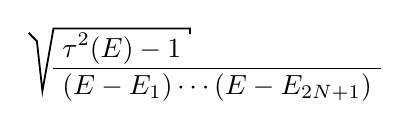
\begin{tikzpicture}[baseline=0pt]
\node[anchor=south west,inner xsep=3pt,inner ysep=1.5pt] (num) at (0,0)
  {$\displaystyle\tau^2(E)-1$};
\node[anchor=north west,inner xsep=3pt,inner ysep=1.5pt] (den) at (0,0)
  {$\displaystyle(E-E_1)\cdots(E-E_{2N+1})$};
\draw (den.north west) -- (den.north east);
\draw[line width=.65pt] (-9pt,13pt)--(-6pt,10pt)--(-4pt,-8pt)
  -- (num.north west) -- (num.north east) -- ([yshift=-2pt]num.north east);
\end{tikzpicture}}\endgroup
\qquad\text{— однозн. ф-я.}
\]
\Unclear{GELFAND-P000567}{root-scope}{Верхняя черта корня доходит только до конца числителя. Нижний угол корня опускается до знаменателя. Область действия корня не установлена однозначно.}
\end{GelfandAdjacentEvidence}
\begin{GelfandAdjacentEvidence}{GELFAND-P000567}{2}

Рассм. ур-е
\begin{gather*}
-\Psi''+u(x)\Psi=E\Psi,\qquad \Psi(x+T)=\lambda\Psi(x)\\
u(x+T)=u(x)
\end{gather*}
Пусть \(\chi=-i\,\Psi'/\Psi\).

\(1^\circ.\quad \chi\) не зависит от \(x_0,\quad\chi=\chi(x,E)\).

\(2^\circ.\quad \chi(x+T)=\chi(x).\)

\(3^\circ.\quad -i\chi'+\chi^2+u-E=0.\)

\(\chi=\chi_R+i\chi_I\) на разреш. зоне — потом аналит. продолж. по \(E\).
\[
4^\circ.\quad\chi_I=\frac12\,\chi_R'/\chi_R.
\]
\begin{gather*}
5^\circ.\quad\chi(x,E)\sim k+\sum_{n=1}^{\infty}\frac{\chi_n(x)}{(2k)^n},
\qquad E=k^2\\
\chi_n=P_n(u,u',\ldots,u^{(n)})\text{ — полином}
\end{gather*}
(послед. опр. из асимпт. равенства)
\[
4^\circ\Rightarrow6^\circ.\quad\chi_R(x,E)\sim k+
\sum_{n=0}^{\infty}\frac{\chi_{2n+1}(x)}{(2k)^{2n+1}}
\]
\[
7^\circ.\quad\Psi(x,x_0,E)=
\sqrt{\frac{\chi_R(x_0,E)}{\chi_R(x,E)}}\cdot
\exp\left[i\int_{x_0}^x\chi_R(t,E)\,dt\right].
\]
\Unclear{GELFAND-P000567}{exponent-overwrites}{В числителе у \(\chi_R\) переписан нижний индекс. В показателе переписаны \(t\), \(E\) и последний \(t\) в \(dt\). Прежние штрихи не установлены.}
\end{GelfandAdjacentEvidence}
\begin{GelfandAdjacentEvidence}{GELFAND-P000567}{3}

\[
7^\circ\Rightarrow8^\circ.\quad|\Psi|^2=\chi_R(x_0,E)/\chi_R(x,E)
\qquad\text{\uwave{в разреш. зоне}}
\]
\(9^\circ.\quad\) \sout{[…]}
\Unclear{GELFAND-P000567}{phase-old}{Перед \(\lambda\) густо зачёркнута запись. Видны фрагменты, похожие на знак равенства и \(p(E)\). Точное чтение не установлено.}
\end{GelfandAdjacentEvidence}
\begin{GelfandAdjacentEvidence}{GELFAND-P000567}{4}

\[
\lambda=e^{ip(E)}\quad\Rightarrow\quad
p(E)=\int_{x_0}^{x_0+T}\chi_R(x,E)\,dx+2\pi n.
\]
Интеграл — функционал от \(u\) с \uwave{асимпт. разложением}. Ур-е Эйлера для него — \uwave{ур-я КдФ},

Разр. и запр. зоны — где \(|\lambda|=1\)
\Unclear{GELFAND-P000567}{old-ordinal}{Слева от «10°» зачёркнут прежний номер с верхним кружком. Видны вертикальный штрих и петля. Точные цифры не установлены.}
\end{GelfandAdjacentEvidence}
\begin{GelfandAdjacentEvidence}{GELFAND-P000567}{5}

\[
10^\circ.\quad\frac{\delta p(E)}{\delta u(x)}=-\frac12\frac1{\chi_R(x,E)}
\]
(лев. часть ур-я Эйлера для КдФ).
\[
11^\circ.\quad\chi(x,E)=
\frac{\sqrt{1-\tau^2(E)}}{\alpha_{21}(x,E)}+
\frac i2\frac{\alpha_{11}(x,E)-\alpha_{22}(x,E)}{\alpha_{21}(x,E)}
\]
Грубая идея: соб. знач. получ. из квадр. ур-я
\[
12^\circ.\quad\text{Пусть}\quad R(E)=\prod_1^{2N+1}(E-E_j).
\qquad\text{Тогда}
\]
\[
\chi(x,E)=\frac{\sqrt{R(E)}}{P(E,x)}-\frac i2\frac{P'_x}{P},
\]
где \(P\) — многочлен по \(E\) степени \(N\).
\Unclear{GELFAND-P000567}{polynomial-prime}{После \(P'_x\) в числителе виден густой штрих, похожий на начало скобки. Его значение не установлено.}
\end{GelfandAdjacentEvidence}



\Needspace{7\baselineskip}
\begin{GelfandAdjacentEvidence}{GELFAND-P000568}{1}
\SourcePage{GELFAND-P000568}{unlabelled}
\[
P(E,x)=\prod_{j=1}^{N}(E-\gamma_j(x)).
\]
\uuline{Задача Г.} Пусть \(R\) и \(P\) — целые ф-и 1-го пор. роста. Тогда им соотв. потенциалы \(u(x)\). Какие?

класс потенциалов (не обяз. периодических).
\noindent\hfill\rule{1.1cm}{.32pt}\enspace\(\cdot\)\enspace\rule{.9cm}{.32pt}\par
\underline{Дубровин.}

\(\Gamma_N\) — рим. пов. \(\sqrt{R(E)}\), \(\chi(x,E)\) — алгебр. ф-я на этой поверхности

\underline{Теорема}: \(\Psi(x,x_0,E)\) однозначная ф-я на \(\Gamma_N\),
мером. на \(\Gamma_N\setminus\infty\), имеет \(N\) нулей и \(N\) полюсов.
\Unclear{GELFAND-P000568}{bloch-separator}{После первого \(x\) написана запятая. Над ней густо зачёркнут небольшой знак. Прежнее чтение не установлено.}
\end{GelfandAdjacentEvidence}

Полюса в \uwave{\mbox{$E=\gamma_i(x_0)$}},
нули над \(E=\gamma_i(x)\).


\Needspace{7\baselineskip}
\begin{GelfandAdjacentEvidence}{GELFAND-P000569}{1}
\SourcePage{GELFAND-P000569}{unlabelled}
\uuline{\mbox{$30/\underline{\overline{\mathrm{IX}}}-74$}.}\qquad
\uwave{Сем. Гельфанда.}

\uuline{Поляков.}\quad\uwave{Об элементарных частицах.}\quad\uwave{Поля Янга-Миллса.}
\hfill(разностный аналог).\par

\uuline{Грэм Сигал.}\qquad\underline{A work of \uuline{Dusa Mc Duff} о конфигур. пр-ве.}
\[
\mathbb R^n,\qquad
C_k(\mathbb R^n)=\{\text{subsets of }\mathbb R^n\text{ with }k
\text{ points (no ordered)}\}.
\]
С топ. точки зрения оно не вполне тривиально.
\SourceFigure{GELFAND-P000569}{point-axes}{%
\par\smallskip
\begingroup\color{black}\GelfandFitDiagram{\begin{tikzpicture}[x=.80cm,y=.75cm]
\draw (-1.46,-.03)--(1.45,.04);
\draw (1.45,.04)--(1.31,.11) (-1.46,-.03)--(-1.33,-.11);
\draw (0,-.87)--(.02,1.47);
\draw[line width=.70pt] (-.92,.91) circle (1.48pt) (.98,.92) circle (1.48pt);
\fill (1.36,-.97) circle (1.50pt);
\end{tikzpicture}}\endgroup\par}
\end{GelfandAdjacentEvidence}
\begin{GelfandAdjacentEvidence}{GELFAND-P000569}{2}

\sout{[…]\ \mbox{$f_S$}}
\Incomplete{GELFAND-P000569}{field-old}{Левая часть зачёркнутой записи не читается.}
\end{GelfandAdjacentEvidence}
\begin{GelfandAdjacentEvidence}{GELFAND-P000569}{3}

\Unclear{GELFAND-P000569}{field-old-fragment}{В конце зачёркнутой записи предположительно \(f_S\).}
\end{GelfandAdjacentEvidence}
\begin{GelfandAdjacentEvidence}{GELFAND-P000569}{4}

\par\smallskip\noindent
\begingroup\color{black}\GelfandFitDiagram{\begin{tikzpicture}[x=1cm,y=.85cm,every node/.style={inner sep=1pt,anchor=west}]
\node (map) at (2.58,.81) {стр. отобр. \(f_S:\mathbb R^n\longrightarrow\mathbb R^n\cup\infty\)};
\node at (0,0) {\(S\subset\mathbb R^n\)};
\node at (0,-.69) {конечное.};
\node (by) at (1.72,0) {по нему};
\draw[->] (by.east) .. controls +(1,.05) and +(-.32,-.46) .. (map.west);
\draw (0.20,-.36)--(.28,-.49);
\end{tikzpicture}}\endgroup
\par
\Unclear{GELFAND-P000569}{map-verb}{Сокращение перед «отобр.» читается как «стр.». К нему снизу направлена стрелка.}
\end{GelfandAdjacentEvidence}
\begin{GelfandAdjacentEvidence}{GELFAND-P000569}{5}

\Unclear{GELFAND-P000569}{german-word}{Конец слова слит со стрелкой. Предположительно «по нему», возможно «по немцу».}
\end{GelfandAdjacentEvidence}
\begin{GelfandAdjacentEvidence}{GELFAND-P000569}{6}

\(E\) — напр. поля (электр.), созд. единичн. зарядами в точках \(x\in S\). Получ. вектор \(E\in\mathbb R^n\cup\infty\)
\SourceFigure{GELFAND-P000569}{charge-vector}{%
\par\smallskip
\begingroup\color{black}\GelfandFitDiagram{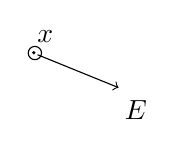
\begin{tikzpicture}[x=.77cm,y=.72cm,every node/.style={inner sep=1pt}]
\draw (0,0) circle (2.4pt);
\fill (-.018,.006) circle (.65pt);
\draw[->] (.045,-.03)--(1.38,-.61);
\node[above] at (.17,.13) {$x$};
\node[below right] at (1.43,-.78) {$E$};
\end{tikzpicture}}\endgroup\par}
\end{GelfandAdjacentEvidence}
\begin{GelfandAdjacentEvidence}{GELFAND-P000569}{7}

В точках \(x\in S\) будет \(\infty\).
\hfill\uwave{\mbox{$\infty\longrightarrow0$}}\par
\[
f_S:\mathbb R^n\cup\infty\longrightarrow\mathbb R^n\cup\infty
\]
Получ. отобр.
\[
\begingroup\color{black}\GelfandFitDiagram{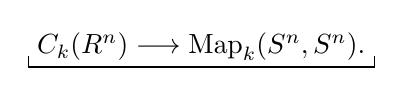
\begin{tikzpicture}[baseline=(mapping.base)]
\node[inner xsep=3pt,inner ysep=2pt] (mapping)
 {$C_k(\mathbb R^n)\longrightarrow\mathrm{Map}_k(S^n,S^n).$};
\draw ([yshift=4pt]mapping.south west) -- (mapping.south west) -- (mapping.south east)
      -- ([yshift=4pt]mapping.south east);
\end{tikzpicture}}\endgroup
\qquad(\text{\uwave{отобр. степени \mbox{$k$}}}).
\]
(Когда далеко, то все \(k\) точек восприн. как одна).
\Unclear{GELFAND-P000569}{far-overwrites}{Буква \(k\) и конец «точек» переписаны. Старые штрихи не читаются.}
\end{GelfandAdjacentEvidence}
\begin{GelfandAdjacentEvidence}{GELFAND-P000569}{8}

Точка, соотв. длинному вектору, — вблизи одного из \(k\) зарядов

— и такие есть.
\Unclear{GELFAND-P000569}{such-word}{В середине «такие» густо переписана буква. Прежние штрихи не читаются.}
\end{GelfandAdjacentEvidence}
\begin{GelfandAdjacentEvidence}{GELFAND-P000569}{9}

\(C_k(\mathbb R^n)\) — хорошая аппрокс. \(\mathrm{Map}_k(S^n,S^n)\)!! (в изв. смысле)

Хорошая аппр. при больших \(k\).
\[
H_i(C_k(\mathbb R^n))\underset{\cong}{\longrightarrow}H_i(\mathrm{Map}_k)
\]
\hfill при \(i\ll k\)\qquad (много док-в есть, в частности Сигала)\par
\Unclear{GELFAND-P000569}{homology-arrow-lower-mark}{Под стрелкой волна над двумя чертами, по форме \(\cong\).}
\end{GelfandAdjacentEvidence}
\begin{GelfandAdjacentEvidence}{GELFAND-P000569}{10}

\uwave{Inventiones}
\Unclear{GELFAND-P000569}{invection-word}{Подчёркнутое слово читается «Inventiones». Конечные буквы соединены.}
\end{GelfandAdjacentEvidence}



\Needspace{7\baselineskip}
\begin{GelfandAdjacentEvidence}{GELFAND-P000570}{1}
\SourcePage{GELFAND-P000570}{unlabelled}
Будет рассказ. обобщение этой теор. (принадл. \sout{[…]} Dusa Mc Duff)
\Incomplete{GELFAND-P000570}{attribution-old}{Перед именем «Dusa Mc Duff» зачёркнута короткая запись. Она не читается.}
\end{GelfandAdjacentEvidence}
\begin{GelfandAdjacentEvidence}{GELFAND-P000570}{2}

\noindent\hfill\rule{.66cm}{.32pt}\enspace\rule{.64cm}{.32pt}\par
\uuline{Фукс.}\quad \(C_k(\mathbb R^n)\) даёт разные классиф. пр-ва.
\Unclear{GELFAND-P000570}{fuchs-overwrite}{В «Фукс» начальная буква переписана плотным штрихом. Прежние штрихи не установлены.}
\end{GelfandAdjacentEvidence}
\begin{GelfandAdjacentEvidence}{GELFAND-P000570}{3}

\noindent\hfill\rule{.72cm}{.32pt}\enspace\(\cdot\)\enspace\rule{.91cm}{.32pt}\par
\uwave{2 сорта вопросов возникает}:

Правое не зав. от \(k\) (\(\approx\)), слева перех. к пределу по \(k\).
\Unclear{GELFAND-P000570}{limit-overwrite}{В слове «пределу» переписана середина. Прежние штрихи не читаются.}
\end{GelfandAdjacentEvidence}
\begin{GelfandAdjacentEvidence}{GELFAND-P000570}{4}

(гомот. экв.)

\(C_k^\pm(\mathbb R^n)\qquad\) finite subsets с зарядами разн. знаков

топология — если 2 разноим. заряда сближ., то они пропадают.

Много компонент (общ. заряд), \(-\infty<k<+\infty\)

Не сильно зависит от \(k\).
\[
C_k^\pm(\mathbb R^n)\underset{2}{\simeq}\mathrm{Map}_k(S^n,S^n)
\]
\Unclear{GELFAND-P000570}{signed-comparison}{Под знаком \(\simeq\) виден отдельный знак в форме цифры \(2\). Его смысл не установлен.}
\end{GelfandAdjacentEvidence}
\begin{GelfandAdjacentEvidence}{GELFAND-P000570}{5}

\uwave{очень хорошая аппрокс.} (гипотеза). или
\Unclear{GELFAND-P000570}{hypothesis-old}{После «гипотеза» густые пересекающиеся штрихи. Предположительное чтение «или».}
\end{GelfandAdjacentEvidence}
\begin{GelfandAdjacentEvidence}{GELFAND-P000570}{6}

Есть пр-во \(Y_n,\qquad\dim Y_n=2n\),
\[
\underline{C_k^\pm(\mathbb R^n)\simeq\mathrm{Map}_k(S^n,Y_n)}.
\]
\Unclear{GELFAND-P000570}{target-relation}{Верхний штрих знака переписан. Видимая волна над чертой передана \(\simeq\).}
\end{GelfandAdjacentEvidence}
\begin{GelfandAdjacentEvidence}{GELFAND-P000570}{7}

\Unclear{GELFAND-P000570}{target-overwrite}{В последнем \(Y_n\) буква \(Y\) переписана. Прежние штрихи не читаются.}
\end{GelfandAdjacentEvidence}
\begin{GelfandAdjacentEvidence}{GELFAND-P000570}{8}

\underline{\(C_k(M)\)}\qquad \underline{\(M\) — мн-зие}

Что вместо \(\mathrm{Map}(S^n,S^n)\)?
\[
C_k(M)\longrightarrow\Gamma(T_M^{\mathrm{comp}}),
\]
\uwave{\mbox{$\infty$} добавл. в каждом слое}. (все слои компактифицированы).

На \sout{[…]} бесконечности можно считать \(0\) (с комп. носит.)
\Unclear{GELFAND-P000570}{infinity-old}{После «На» зачёркнут небольшой петлеобразный знак. Чтение не установлено.}
\end{GelfandAdjacentEvidence}
\begin{GelfandAdjacentEvidence}{GELFAND-P000570}{9}

\[
C_k(M)\longrightarrow\Gamma_k^{\mathrm{cpt}}(T_M^{\mathrm{comp}})
\]
инд. гомол. изом. при \(i\ll k\).

(Считается, что электр. поле имеет конечн. протяж. — тогда всё стр.)

\uline{Наиболее интересен метод док-ва, а не утверждение}.

\(U\subset M\)\quad мал. кусок \(M\).
\qquad \(C_k(U)\)\ \sout{[…]}\ \(C_k(M)\).
\Unclear{GELFAND-P000570}{inclusion-old}{Между \(C_k(U)\) и \(C_k(M)\) густо зачёркнут знак. Его чтение не установлено.}
\end{GelfandAdjacentEvidence}
\begin{GelfandAdjacentEvidence}{GELFAND-P000570}{10}

Хотелось бы получ. \(C_k(M)\), объединяя \(C_k(U)\).
\SourceFigure{GELFAND-P000570}{overlap-path}{%
\par\smallskip
\begingroup\color{black}\GelfandFitDiagram{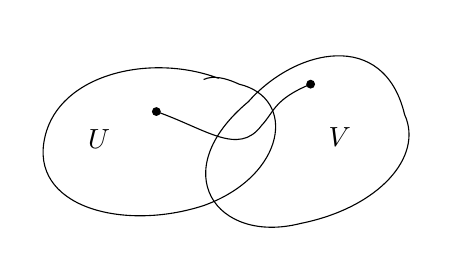
\begin{tikzpicture}[x=.79cm,y=.74cm,every node/.style={inner sep=1pt}]
\draw (1.35,1.12) .. controls (.25,1.56) and (-1.21,1.19) .. (-1.44,.12)
  .. controls (-1.71,-1.08) and (-.19,-1.52) .. (1.12,-1.06)
  .. controls (2.43,-.55) and (2.62,.78) .. (1.68,1.02)
  .. controls (1.48,1.12) and (1.27,1.18) .. (1.11,1.10);
\draw (4.34,.50) .. controls (4.01,1.98) and (2.58,1.63) .. (1.83,.72)
  .. controls (.48,-.48) and (1.31,-1.74) .. (2.67,-1.37)
  .. controls (3.93,-1.10) and (4.65,-.22) .. (4.34,.50);
\draw (.35,.55) .. controls (1.15,.25) and (1.67,-.22) .. (2.04,.31)
  .. controls (2.25,.55) and (2.24,.76) .. (2.83,1.02);
\fill (.35,.55) circle (1.6pt) (2.83,1.02) circle (1.6pt);
\node at (-.57,.08) {$U$};
\node at (3.30,.11) {$V$};
\end{tikzpicture}}\endgroup\par}
\end{GelfandAdjacentEvidence}
\begin{GelfandAdjacentEvidence}{GELFAND-P000570}{11}

\[
C(M)\underset{\text{разрывно}}{\longrightarrow} C(U)\times C(V)
\]
\Unclear{GELFAND-P000570}{restriction-note}{Слово «разрывно» находится под формулой и над следующей строкой.}
\end{GelfandAdjacentEvidence}

Пусть \(U,V\) — мн-зия с краем.

\(\overline C(U)\) — факторпр-во \(C(U)\)
\[
S_1\sim S_2\quad\Leftrightarrow\quad S_1\cap\overset{\circ}U=S_2\cap\overset{\circ}U
\]
(точки на крае пропадают)

\underline{Теор.}\quad \(U\) — мн. с краем (непустым)
\[
\Rightarrow\quad\overline C(U)\underset{\simeq}{\longrightarrow}
\Gamma(TU^{\mathrm{comp}})\qquad(\text{гомотопич. эквив.}).
\]
\underline{Док-во.}\quad\uuline{Случ.~1.}\qquad \(U=\) ед. диск.

\uwave{Лев. часть}: \(C_\varepsilon(U)\) — конфигур. с расст. \(>\varepsilon\).
Остаются конфигур. \(\leqslant1\) \uwave{частиц}.

пр. часть\qquad \(\mathrm{Map}(U,S^n)\simeq S^n\)

Радиальн. раст. \(\longrightarrow S^n\) (выдавл. на границу)


\Needspace{7\baselineskip}
\begin{GelfandAdjacentEvidence}{GELFAND-P000571}{1}
\SourcePage{GELFAND-P000571}{unlabelled}
\SourceFigure{GELFAND-P000571}{cover-circles}{%
\par\smallskip
\begingroup\color{black}\GelfandFitDiagram{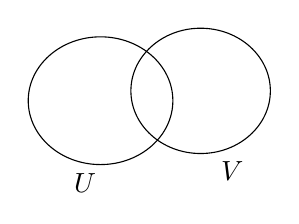
\begin{tikzpicture}[x=.82cm,y=.78cm,every node/.style={inner sep=1pt}]
\draw (0,0) ellipse (1.12 and 1.04);
\draw (1.55,.16) ellipse (1.08 and 1.02);
\node[below] at (-.24,-1.14) {$U$};
\node[below] at (2.04,-.94) {$V$};
\end{tikzpicture}}\endgroup\par}
\end{GelfandAdjacentEvidence}
\begin{GelfandAdjacentEvidence}{GELFAND-P000571}{2}

\SourceFigure{GELFAND-P000571}{cover-diagram}{%
\par\smallskip
\begingroup\color{black}\GelfandFitDiagram{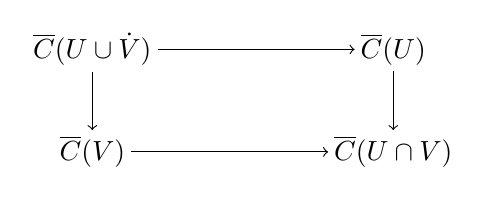
\begin{tikzpicture}[x=.84cm,y=.84cm,every node/.style={inner sep=2pt}]
\node (A) at (0,0) {$\overline C(U\cup\dot V)$};
\node (B) at (4.55,0) {$\overline C(U)$};
\node (C) at (0,-1.55) {$\overline C(V)$};
\node (D) at (4.55,-1.55) {$\overline C(U\cap V)$};
\draw[->] (A)--(B);
\draw[->] (A)--(C);
\draw[->] (B)--(D);
\draw[->] (C)--(D);
\end{tikzpicture}}\endgroup\par
Над \(V\) в левом верхнем углу стоит точка. Её значение не установлено. Нижняя стрелка направлена вправо.}
\end{GelfandAdjacentEvidence}
\begin{GelfandAdjacentEvidence}{GELFAND-P000571}{3}

есть корр. опр. отобр. и если 2 точки из \(\overline C(U)\) и \(\overline C(V)\) опр. одну в
\(\overline C(U\cap V)\), то \sout{это} опр. точку из \(\overline C(U\cup V)\).
\Unclear{GELFAND-P000571}{cancelled-pronoun}{После «то» зачёркнуто «это».}
\end{GelfandAdjacentEvidence}
\begin{GelfandAdjacentEvidence}{GELFAND-P000571}{4}

\SourceFigure{GELFAND-P000571}{section-square}{%
\par\smallskip
\begingroup\color{black}\GelfandFitDiagram{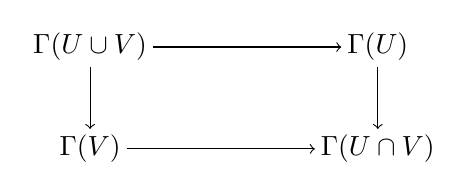
\begin{tikzpicture}[x=.84cm,y=.84cm,every node/.style={inner sep=2pt}]
\node (A) at (0,0) {$\Gamma(U\cup V)$};
\node (B) at (4.35,0) {$\Gamma(U)$};
\node (C) at (0,-1.54) {$\Gamma(V)$};
\node (D) at (4.35,-1.54) {$\Gamma(U\cap V)$};
\draw[->] (A)--(B);
\draw[->] (A)--(C);
\draw[->] (B)--(D);
\draw[->] (C)--(D);
\end{tikzpicture}}\endgroup\par}
\end{GelfandAdjacentEvidence}
\begin{GelfandAdjacentEvidence}{GELFAND-P000571}{5}

\uwave{Св-ва накр. гомотопии}.
\Unclear{GELFAND-P000571}{homotopy-phrase}{Среднее сокращение читается «накр.».}
\end{GelfandAdjacentEvidence}

\noindent\hfill\rule{.95cm}{.32pt}\enspace\(\cdot\)\enspace\rule{1.05cm}{.32pt}\par
аналог. теор. о \(C_k(M)\) опускается.

\noindent\hfill\rule{1.05cm}{.32pt}\enspace\(\cdot\)\enspace\rule{.89cm}{.32pt}\par
\underline{След. раз}: Поляков или Дубровин.


\Needspace{7\baselineskip}
\begin{GelfandAdjacentEvidence}{GELFAND-P000572}{1}
\SourcePage{GELFAND-P000572}{unlabelled}
\underline{7/X--74.}\qquad\underline{Сем. Гельфанда.}

\underline{Кушниренко.}\qquad \(f(z_1,\ldots,z_n)=\sum a_m z^m\)

\(0\) — особ. точка. (ряд без своб. и линейного членов).

Число Милнора \(\mu(f)\) \(=\) кратность нулевого реш.
\[
\frac{\partial f}{\partial z_1}=0,\ldots,\frac{\partial f}{\partial z_n}=0.
\]
\noindent\hfill\begin{minipage}{.47\linewidth}
\noindent\vrule width .35pt\hspace{1pt}\vrule width .35pt\enspace
\begin{minipage}{.88\linewidth}
— \underline{\(\max\)} \uwave{число} \sout{[\ldots]} \sout{[\ldots]} \uwave{реш.}\\
\(\dfrac{\partial f}{\partial z_i}=\varepsilon_i\)\\
\uwave{при малом \(\varepsilon\)}.
\end{minipage}
\end{minipage}\par
\Incomplete{GELFAND-P000572}{margin-old}{В правой заметке после «число» и перед «реш.» две зачёркнутые группы. Остатки штрихов видны, полное чтение не установлено.}
\end{GelfandAdjacentEvidence}
\begin{GelfandAdjacentEvidence}{GELFAND-P000572}{2}


Задача: вычислить \(\mu(f)\) по коэфф. ряда Тейлора.

\underline{2-мерн. случай.}\quad(\underline{\(n=2\)})
\SourceFigure{GELFAND-P000572}{newton-polygon}{%
\par\smallskip
\begingroup\color{black}\GelfandFitDiagram{\begin{tikzpicture}[x=.87cm,y=.78cm,every node/.style={inner sep=1.4pt}]
\draw (0,-.16)--(0,5);
\draw[->] (-.35,0)--(6.1,0) node[right] {$m_2$};
\node[left] at (-.64,4.93) {$m_1$};
\draw (0,2.65)--(.56,1.96)--(1.28,1.13)--(2.7,.49)--(4.35,0);
\foreach \point in {(0,2.65),(.56,1.96),(1.28,1.13),(2.7,.49),(4.35,0)}
  \fill \point circle (2pt);
\draw (3.52,.56) circle (1.5pt);
\draw (1.52,1.57) circle (1.4pt);
\node[above] at (.48,2.7) {$\alpha$};
\node[above] at (.95,2.04) {$\beta$};
\node[above] at (1.7,1.69) {$\gamma\,?$};
\draw (-.19,.05) .. controls (-.79,.88) and (-.73,1.95) .. (-.12,2.62);
\node[left] at (-.66,1.25) {$a$};
\node[left] at (-.68,2.46) {$a$};
\draw (0,.15)--(.34,.59) (0,.7)--(.55,1.4) (0,1.25)--(.32,1.72)
      (.52,.12)--(.94,.64) (.87,.07)--(1.22,.51) (1.36,.07)--(1.73,.35)
      (1.86,.04)--(2.13,.25) (2.21,.04)--(2.48,.23) (2.58,.05)--(2.82,.3);
\node at (.37,.81) {$S$};
\draw (0,-.12)--(0,-2.76) (4.35,-.11)--(4.35,-2.55);
\draw[<->] (0,-2.45)--(4.17,-2.32) node[midway,below] {$b$};
\draw[<->] (1.43,-1.19)--(1.43,.47);
\node[anchor=west,align=left] at (1.72,-1.19) {Здесь нет отмеч.\\мономов};
\end{tikzpicture}}\endgroup\par
Третья подпись переписана. По форме и по следующей формуле вероятна \(\gamma\), но чтение не окончательное. Две небольшие отметки над ломаной сохранены.}
\end{GelfandAdjacentEvidence}
\begin{GelfandAdjacentEvidence}{GELFAND-P000572}{3}

\uwave{вып. ломаная}
\[
\nu(f)=2S-a-b+1.
\]
\uuline{Теорема}: \quad 1) \(\mu(f)\geqslant\nu(f)\)

2) \(\mu(f)=\nu(f)\), если вып. нек-рые усл. невырожденности

\(\beta^2\ne 4\alpha\gamma\) \quad
\((\alpha,\beta,\gamma\) — коэффициенты при соотв. мономах\()\).

(в общ. случае \(\ne0\) дискриминант \uwave{левого ребра}.)

\hfill \(\searrow\) на ребре по сущ. многочлен 1-го перем.\par

\uuline{\(n=3.\)}
\[
\nu(f)=3!V-2!(S_{12}+S_{13}+S_{23})+1!(L_1+L_2+L_3)-1.
\]
\(S_{12}\) — площ., к-рая получ. на плоскости.
\SourceFigure{GELFAND-P000572}{coordinate-section}{%
\par\smallskip
\begingroup\color{black}\GelfandFitDiagram{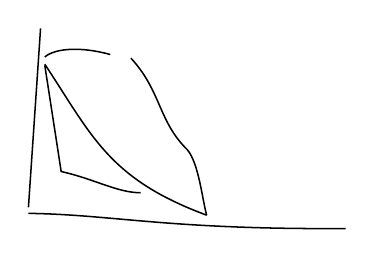
\begin{tikzpicture}[x=.77cm,y=.77cm,line width=.55pt]
\draw (0,.1)--(.2,3.05);
\draw (0,0).. controls (1.4,-.02) and (2.3,-.27) .. (5.23,-.25);
\draw (.27,2.58).. controls (.45,2.73) and (.88,2.75) .. (1.35,2.62);
\draw (1.69,2.56).. controls (2.19,2.02) and (2.14,1.52) .. (2.62,1.05)
      .. controls (2.81,.83) and (2.87,.21) .. (2.94,-.03);
\draw (.27,2.46).. controls (1.05,1.28) and (1.32,.57) .. (2.94,-.03);
\draw (.27,2.44)--(.54,.69).. controls (1.08,.57) and (1.47,.34) .. (1.85,.34);
\end{tikzpicture}}\endgroup\par
Пространственная связь контуров передана схематически, как в рукописи.}
\end{GelfandAdjacentEvidence}
\begin{GelfandAdjacentEvidence}{GELFAND-P000572}{4}

\Unclear{GELFAND-P000572}{section-detached-stroke}{Между формулой для \(\nu\) и рисунком виден короткий отдельный косой штрих. Его функция не установлена.}
\end{GelfandAdjacentEvidence}


\uuline{Теорема}: \quad 1) \(\mu(f)\geqslant\nu(f)\)

2) усл. невыр. \(\Rightarrow\) \underline{рав-во}.

\hspace{1.5em}(вып. почти всегда)


\Needspace{7\baselineskip}
\begin{GelfandAdjacentEvidence}{GELFAND-P000573}{1}
\SourcePage{GELFAND-P000573}{unlabelled}
\SourceFigure{GELFAND-P000573}{face-cone}{%
\par\smallskip
\begingroup\color{black}\GelfandFitDiagram{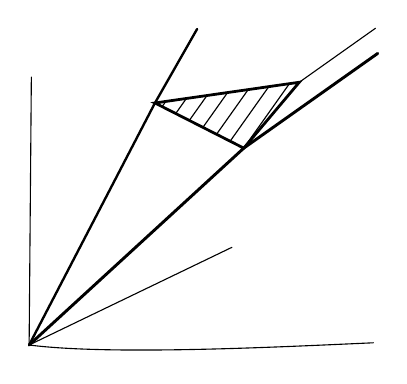
\begin{tikzpicture}[x=.94cm,y=.94cm,line cap=round]
\draw (.03,3.62)--(0,0).. controls (1.1,-.14) and (3.3,-.03) .. (4.65,.03);
\draw (0,0)--(2.74,1.32);
\draw[line width=.85pt] (0,0)--(1.7,3.27)--(2.27,4.27);
\draw[line width=1.05pt] (0,0)--(2.9,2.66)--(4.71,3.94);
\draw[line width=.4pt] (2.9,2.66)--(3.65,3.55)--(4.68,4.28);
\begin{scope}
\clip (1.7,3.27)--(3.65,3.55)--(2.9,2.66)--cycle;
\foreach \x in {1.30,1.55,1.80,2.05,2.30,2.55,2.80,3.05,3.30}
  \draw[line width=.42pt] (\x,2.52)--++(.9,1.27);
\end{scope}
\draw[line width=1pt] (1.7,3.27)--(3.65,3.55)--(2.9,2.66)--cycle;
\end{tikzpicture}}\endgroup\par
Штрихованный участок между верхними лучами. Утолщённые и повторные штрихи переданы схематически, точные направления продолжений не установлены.}
\end{GelfandAdjacentEvidence}
\begin{GelfandAdjacentEvidence}{GELFAND-P000573}{2}

\[
z_i\frac{\partial f_\Delta}{\partial z_i}
\]
\uwave{\(f_\Delta\) — соотв. мономам грани.}
\[
\dim_{\mathbb C}\mathbb C[P(\Delta)]\big/\left(z_i\frac{\partial f}{\partial z_i}\right)<\infty.
\]
\hfill усл. невырожд.\par

\underline{Док-во}: коммут. алгебра. Использ., что \(\mathbb C[P(\Delta)]\) — кольцо Коэна–Маколея (Хохстер).

\uuline{Арнольд}.
\[
\sum_{\substack{x,y:\left\{\begin{smallmatrix}P_n(x,y)=0\\Q_n(x,y)=0\end{smallmatrix}\right.}}^{n^2}
\frac{R_{n-4}(x,y)}{\det\frac{\partial(P_n\,Q)}{\partial(x,y)}}=0.
\]
\Unclear{GELFAND-P000573}{jacobian-denominator}{В числителе якобиана после \(P_n\) видно \(Q\). Отдельная запятая не видна, возможный индекс у \(Q\) сливается с хвостом буквы и скобкой. В условиях суммы отдельно написано \(Q_n\).}
\end{GelfandAdjacentEvidence}
\begin{GelfandAdjacentEvidence}{GELFAND-P000573}{3}

\(P_n(x,y)\), \(Q_n(x,y)\) — 2 \uwave{многочлена}.

(\underline{\(R\) — произв. многочлен} степ. \(\le n-4\))

\hfill\uwave{\(\sum\) по всем нулям}.\par

\uuline{Поляков}. Рассм. \(\mathbb Z^2\) и ф-ю от направл. ребра, соед. соседн. верш.
\SourceFigure{GELFAND-P000573}{yellow-mark}{В растре над «направл.» виден жёлтый значок с тремя полосками. Текст значка отсутствует в изображении, его происхождение не установлено.}
\end{GelfandAdjacentEvidence}
\begin{GelfandAdjacentEvidence}{GELFAND-P000573}{4}

\uwave{Поля Янга–Миллса}.
\[
B_{\tau,\alpha},\quad \tau\in\mathbb Z^2,\quad \alpha\text{ — напр.}
\]
ф-я со зн. в \(\mathrm{SU}(2)\) (или другой комп. гр.).
\SourceFigure{GELFAND-P000573}{edge-directions}{%
\par\smallskip
\begingroup\color{black}\GelfandFitDiagram{\begin{tikzpicture}[x=1cm,y=1cm]
\fill (0,0) circle (1.6pt);
\draw[->] (0,0)--(0,1.54) node[midway,left] {$\beta\,?$};
\draw[->] (0,0)--(1.76,.13) node[near end,below] {$\alpha$};
\node[below] at (0,0) {$\tau$};
\end{tikzpicture}}\endgroup\par
Подпись при вертикальной стрелке похожа на \(\beta\), но форма не вполне ясна. При горизонтальной стрелке читается \(\alpha\).}
\end{GelfandAdjacentEvidence}
\begin{GelfandAdjacentEvidence}{GELFAND-P000573}{5}

\[
F_{\vec\tau,\alpha\beta}
=\quad\begingroup\color{black}\GelfandFitDiagram{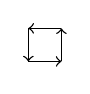
\begin{tikzpicture}[baseline=-.35ex,x=.42cm,y=.42cm,line width=.5pt]
\draw[->] (1,1)--(0,1);
\draw[->] (0,1)--(0,0);
\draw[->] (0,0)--(1,0);
\draw[->] (1,0)--(1,1);
\end{tikzpicture}}\endgroup
\quad\text{циркул.}
=B_{\tau\alpha}B_{\tau+a_\alpha,\beta}B_{\tau+a_\beta,\alpha}^{-1}B_{\tau\beta}^{-1}.
\]
\SourceFigure{GELFAND-P000573}{plaquette}{Стрелки на верхней, левой, нижней и правой сторонах направлены соответственно влево, вниз, вправо и вверх.}
\end{GelfandAdjacentEvidence}
\begin{GelfandAdjacentEvidence}{GELFAND-P000573}{6}

(напряж. \sout{[\ldots]} \(B\)). \(\hookleftarrow\) поля
\Unclear{GELFAND-P000573}{field-word-old}{Старое слово перед \(B\) зачёркнуто, предположительно «контура». Вставка «поля» стоит ниже, от неё проведён штрих.}
\end{GelfandAdjacentEvidence}
\begin{GelfandAdjacentEvidence}{GELFAND-P000573}{7}


Энергия
\[
E=\sum_{\tau,\alpha,\beta}\chi(F_{\tau,\alpha,\beta})
\qquad
Z=\int\prod dB_{\tau,\alpha}\,e^{-\frac1T E[B]}.
\]
\Unclear{GELFAND-P000573}{energy-old}{Над \(F\) виден плотный чёрный участок. Подлежащий знак и его функция не установлены.}
\end{GelfandAdjacentEvidence}
\begin{GelfandAdjacentEvidence}{GELFAND-P000573}{8}

\uwave{\(\chi\) — след.}

Корреляц. ф-и:
\[
\Pi(C)=Z^{-1}\int\prod dB_{\tau\alpha}\,\chi\left[\prod_{(C)}B_{\tau\lambda}\right]
   e^{-\frac1T E(B)}.
\]
\(\alpha,\beta=1\) или \(2\) \hfill \uwave{\(C\) — контур}.

Решётка размера \(N\times N\).

Плоская зад. решается точно.
\begin{gather*}
\widetilde E=\sum_{\tau,\alpha}\chi(g_{\bar\tau}^{-1}g_{\vec\tau+\vec a_\alpha})\\
\widetilde{\widetilde E}
=\sum_{\tau,\alpha}\chi(g_{\bar\tau}^{-1}g_{\bar\tau+\bar a_\alpha} B_{\bar\tau,\alpha})
  \mathord{.}\,+E[B].
\end{gather*}
\Unclear{GELFAND-P000573}{double-tilde-energy}{В строке с двумя тильдами \(B\) стоит внутри скобок после второго \(g\), без видимой запятой между ними. Над индексом \(\tau\) у \(B\) черта. Перед знаком \(+\) виден отдельный маленький штрих у нижнего края строки.}
\end{GelfandAdjacentEvidence}
\begin{GelfandAdjacentEvidence}{GELFAND-P000573}{9}


Теор. поля \(=\) стат. мех. в \(\mathbb R^n\) (евклидовом).

(преобр. Фурье по времени)

\underline{Синай}.
\SourceFigure{GELFAND-P000573}{square-grid}{%
\par\smallskip
\begingroup\color{black}\GelfandFitDiagram{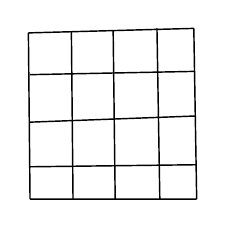
\begin{tikzpicture}[x=.52cm,y=.52cm,line width=.52pt]
\draw (0,0)--(-.04,4.06) (1.05,0)--(1.01,4.10) (2.08,0)--(2.03,4.12)
      (3.17,0)--(3.10,4.17) (4.07,0)--(4,4.17);
\draw (0,0)--(4.07,0) (0,.79)--(4.05,.84) (0,1.88)--(4.03,2.03)
      (0,3.04)--(4.02,3.12) (-.04,4.06)--(4,4.17);
\end{tikzpicture}}\endgroup\par}
\end{GelfandAdjacentEvidence}

\uwave{\(V\) — кон. объём}.
\[
E(\{B_{\tau\alpha}\})=\sum\mathrm{tr}
\left(B_{\tau\alpha}B_{\tau+a_\alpha,\beta}B_{\tau+a_\beta,\alpha}^{-1}B_{\tau,\beta}^{-1}\right)
\]
\[
\underline{\underline{\mathcal M e^{-\beta E}=Z(\beta,V)}}
\]
Считается для 2-мерн. случая.
\[
\ln Z(\beta,V)=V\ln I_0(\beta)
\qquad (I_0(\beta)\text{ — ф-я Бесселя})
\]


\Needspace{7\baselineskip}
\begin{GelfandAdjacentEvidence}{GELFAND-P000574}{1}
\SourcePage{GELFAND-P000574}{unlabelled}
\[
B_{\tau\alpha}=e^{i A_{\tau\alpha}}
\]
\Unclear{GELFAND-P000574}{b-tight}{Первый нижний индекс у \(B\) и у \(A\) читается как \(\tau\).}
\end{GelfandAdjacentEvidence}
\begin{GelfandAdjacentEvidence}{GELFAND-P000574}{2}


\[
\text{\sout{[\ldots]}}\ E=\sum\cos(A_{\tau\alpha}+A_{\tau+a_\alpha,\beta}-\ldots)
\]
\Unclear{GELFAND-P000574}{cancel-e-tight}{Перед \(E\) густо перечёркнут короткий знак. \(\varphi\) возможно, но чтение не установлено.}
\end{GelfandAdjacentEvidence}
\begin{GelfandAdjacentEvidence}{GELFAND-P000574}{3}

\Unclear{GELFAND-P000574}{e-index-tight}{Во втором индексе под знаком косинуса видны \(\tau+a_\alpha\), запятая и \(\beta\).}
\end{GelfandAdjacentEvidence}

\[
\lim_{V\to\infty}\frac{\ln Z(\beta,V)}{V}=f(\beta)
\]
\hfill\uwave{не зависит от выбора гран. условий}.\par

\(f(\beta)\) может иметь особенности — они наз. фаз. переходами.

(\(\approx\) происх. перестройка типичн. конфигураций).

\[
p(\{B_{\tau,\alpha}\})=Z^{-1}e^{-\beta E(\{B_{\tau\alpha}\})}
\qquad\text{— распр. Гиббса.}
\]

Коррел. ф-я — средн. знач. циркуляции по контуру.

\noindent
\begin{tabular}{@{}ll@{}}
Фаз. перех. — & в одной фазе \(\sim\) площади\\
               & в другой \(\sim\) длине.
\end{tabular}


\Needspace{7\baselineskip}
\begin{GelfandAdjacentEvidence}{GELFAND-P000575}{1}
\SourcePage{GELFAND-P000575}{unlabelled}
\sout{[\ldots]}\quad\underline{14/X--74.}\qquad\underline{Сем. Гельфанда.}
\Unclear{GELFAND-P000575}{cancel-date-tight}{Перед датой зачёркнута короткая группа. Чтение «По» возможно, но пересечение штрихов мешает разобрать буквы.}
\end{GelfandAdjacentEvidence}
\begin{GelfandAdjacentEvidence}{GELFAND-P000575}{2}


\uuline{Грэм Сигал}.

\uuline{Classifying space of category.}

\(\mathcal C\) — category, \qquad \(|\mathcal C|\) is top. space

\uwave{Objects} — points

\uwave{Morphisms} — 1-dim symplex.

\uwave{Compositions — ?}
\SourceFigure{GELFAND-P000575}{graph-tight}{%
\par\smallskip
\begingroup\color{black}\GelfandFitDiagram{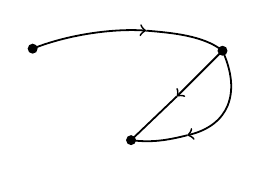
\begin{tikzpicture}[x=.88cm,y=.88cm,line width=.65pt]
\coordinate (A) at (0,1.32);
\coordinate (B) at (2.74,1.29);
\coordinate (C) at (1.42,0);
\draw[->] (A).. controls (.58,1.55) and (1.24,1.61) .. (1.64,1.58);
\draw (1.64,1.58).. controls (2,1.55) and (2.47,1.51) .. (B);
\draw[->] (B)--(2.08,.63);
\draw (2.08,.63)--(C);
\draw[->] (B).. controls (3.02,.67) and (2.82,.21) .. (2.23,.07);
\draw (2.23,.07).. controls (1.95,0) and (1.72,-.04) .. (C);
\foreach \v in {A,B,C} \fill (\v) circle (1.8pt);
\end{tikzpicture}}\endgroup\par}
\end{GelfandAdjacentEvidence}
\begin{GelfandAdjacentEvidence}{GELFAND-P000575}{3}

we have a \uwave{graph}.

It describe not cat. \([?]\)
\Unclear{GELFAND-P000575}{tail-loop}{После «cat.» виден низкий петлеобразный знак. Чтение \(\mathcal C\) предположительно, его форма отличается от ясно написанной буквы выше.}
\end{GelfandAdjacentEvidence}
\begin{GelfandAdjacentEvidence}{GELFAND-P000575}{4}

\hspace{1.1em}(composition!)
\SourceFigure{GELFAND-P000575}{compos-left}{%
\par\smallskip
\begingroup\color{black}\GelfandFitDiagram{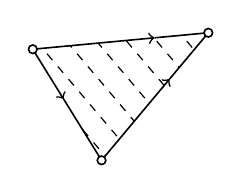
\begin{tikzpicture}[x=.91cm,y=.91cm,line width=.58pt]
\coordinate (A) at (0,1.55);
\coordinate (B) at (2.45,1.78);
\coordinate (C) at (.96,0);
\begin{scope}
\clip (A)--(B)--(C)--cycle;
\foreach \x in {-.5,-.1,.32,.74,1.16,1.58,2}
  \draw[dashed,line width=.43pt] (\x,1.84)--++(1.5,-1.77);
\end{scope}
\draw[->] (A)--(1.7,1.7096);
\draw (1.7,1.7096)--(B);
\draw[->] (A)--(.43,.8557);
\draw (.43,.8557)--(C);
\draw[->] (C)--(1.91,1.1349);
\draw (1.91,1.1349)--(B);
\foreach \v in {A,B,C} \filldraw[fill=white,draw=black] (\v) circle (1.55pt);
\end{tikzpicture}}\endgroup\par}
\end{GelfandAdjacentEvidence}
\begin{GelfandAdjacentEvidence}{GELFAND-P000575}{5}

\uwave{two-symplex} — \uwave{composition} of two morphisms.

\uwave{3 morph.}, and all compos. — \uwave{3-dim symplex}.

\hspace{2em}\fbox{\small which can be composed}\(\,\uparrow\)
\SourceFigure{GELFAND-P000575}{compos-right}{%
\par\smallskip
\begingroup\color{black}\GelfandFitDiagram{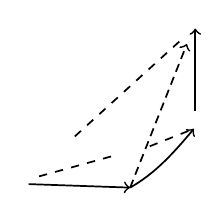
\begin{tikzpicture}[x=.89cm,y=.89cm,line width=.62pt]
\coordinate (A) at (0,0);
\coordinate (B) at (1.45,-.05);
\coordinate (C) at (2.36,.79);
\coordinate (D) at (2.38,2.22);
\draw[->] (A)--(B);
\draw[->] (B).. controls (1.8,.15) and (2.05,.42) .. (C);
\draw[->] (2.38,1.05)--(D);
\draw[->,densely dashed] (B)--(2.26,2);
\draw[dashed] (.15,.11)--(1.27,.42) (1.73,.54)--(C);
\draw[dashed] (.66,.68)--(2.18,2.06);
\end{tikzpicture}}\endgroup\par
Сплошные стрелки и различимые тонкие штрихи переданы схематически. Направления у некоторых наложенных рёбер не установлены.}
\end{GelfandAdjacentEvidence}
\begin{GelfandAdjacentEvidence}{GELFAND-P000575}{6}

etc.

We define \(|\mathcal C|\).

\underline{Diametr. opposed examples.}

\fbox{\small\uwave{Partially}}\(\,\downarrow\)

\uwave{Ordered sets}.

\(\equiv\) categ. with at most one morph. between two objects.

\underline{groups}
\SourceFigure{GELFAND-P000575}{group-tight}{%
\par\smallskip
\begingroup\color{black}\GelfandFitDiagram{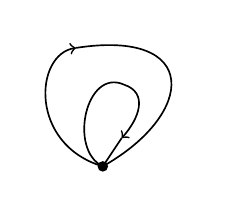
\begin{tikzpicture}[x=.85cm,y=.85cm,line width=.6pt]
\draw[->] (0,0).. controls (-1.11,.33) and (-1.02,1.68) .. (-.4,1.77);
\draw (-.4,1.77).. controls (1.46,2.06) and (1.4,.79) .. (0,0);
\draw[->] (0,0).. controls (-.52,.25) and (-.25,1.48) .. (.32,1.22)
  .. controls (.68,1.1) and (.55,.72) .. (.28,.42);
\draw (.28,.42)--(0,0);
\fill (0,0) circle (1.9pt);
\end{tikzpicture}}\endgroup\par
morphisms \(\cong\) \uwave{elts of group}\par
\uwave{one} object.\par
compos \(=\)\par
\(=\) comp. of elem.}
\end{GelfandAdjacentEvidence}


\noindent\rule{1.45cm}{.32pt}\enspace\(\cdot\)\enspace\rule{1.55cm}{.32pt}\par

\(X\) top space, \qquad \(\{U_\alpha\}_{\alpha\in S}\) — covering \qquad \(U_\alpha\subset X\)

\hspace{8em}\textit{open sets}

\underline{We suppose:}

\uwave{Property:}
\[
U_\alpha\cap U_\beta=\bigcup_{\text{certain }\gamma}U_\gamma.
\]
\[
\alpha\le\beta\quad\underset{\mathrm{def}}{\Longleftrightarrow}\quad U_\alpha\subset U_\beta.
\]
If all sets are contractible then
\(\lvert\mathcal C\rvert\underset{\text{hom. equiv.}}{\simeq}X\).

Добавл. пересечения.


\Needspace{7\baselineskip}
\begin{GelfandAdjacentEvidence}{GELFAND-P000576}{1}
\SourcePage{GELFAND-P000576}{unlabelled}
\underline{Example.}\qquad \(X=S^2\). \hfill \(w=U\cap V\).
\SourceFigure{GELFAND-P000576}{sphere}{%
\par\smallskip
\begingroup\color{black}\GelfandFitDiagram{\begin{tikzpicture}[x=.89cm,y=.89cm,line width=.56pt]
\draw (0,0) ellipse (1.06 and .96);
\draw[dashed] (-1.06,.03).. controls (-.63,.37) and (.64,.36) .. (1.04,.03);
\draw[line width=.85pt] (-1.06,.03).. controls (-.75,-.49) and (.76,-.4) .. (1.04,.06);
\node[above right] at (.78,.72) {$U$};
\node[below] at (-.03,-1.1) {$V$};
\fill (-1.24,.45) circle (1.25pt);
\draw[line width=.32pt] (.05,.96)--(.16,.88);
\begin{scope}[xshift=3.25cm]
\draw (0,0) ellipse (1.12 and 1.22);
\begin{scope}[rotate=13]
\draw[line width=.68pt] (0,-.14) ellipse (1.12 and .46);
\draw[line width=.61pt] (0,-.14) ellipse (1.04 and .30);
\fill (-1.08,-.14) circle (1.2pt);
\draw (1.03,-.12) ellipse (.09 and .12);
\draw[line width=.34pt] (-.66,.15)--(-.48,.22) (.59,-.56)--(.78,-.50);
\end{scope}
\draw[line width=.35pt] (-1.04,.43).. controls (-1.11,.56) and (-.94,.92) .. (-.84,1);
\end{scope}
\end{tikzpicture}}\endgroup\par
В верхней схеме слева от контура видна маленькая отметка. На нижней схеме линии пояса и боковые отметки местами сливаются.}
\end{GelfandAdjacentEvidence}
\begin{GelfandAdjacentEvidence}{GELFAND-P000576}{2}

\SourceFigure{GELFAND-P000576}{interval}{%
\par\smallskip
\begingroup\color{black}\GelfandFitDiagram{\begin{tikzpicture}[x=.85cm,y=.85cm,line width=.55pt]
\fill (0,1.5) circle (1.55pt) (1.3,1.57) circle (1.55pt) (2.6,1.5) circle (1.55pt);
\draw[->] (1.04,1.55)--(.24,1.50);
\draw[->] (1.55,1.56)--(2.36,1.5);
\node[anchor=west,inner sep=0pt] at (0,.82) {\small But \(W\) is not contractible.};
\node[left] at (0,0) {$\lvert\mathcal C\rvert=$};
\draw (0,0)--(2.6,0);
\foreach \x in {0,1.3,2.6} \filldraw[fill=white,draw=black] (\x,0) circle (1.48pt);
\node[right] at (2.83,0) {\small отрезок.};
\end{tikzpicture}}\endgroup\par}
\end{GelfandAdjacentEvidence}
\begin{GelfandAdjacentEvidence}{GELFAND-P000576}{3}

\[
\begin{aligned}
w&=W_1\cup W_2.\\
x_1&\in(W_1\cap W_2)_{\text{comp}}.\\
x_2&\in(W_1\cap W_2)_{\substack{\text{connected}\\\text{comp}}}.
\end{aligned}
\]
\Unclear{GELFAND-P000576}{conn-comp-placed}{Справа от первой скобки читается «comp», от второй — «connected» и под ним «comp».}
\end{GelfandAdjacentEvidence}
\begin{GelfandAdjacentEvidence}{GELFAND-P000576}{4}


\sout{oc?} — \uwave{surface of octahedron}.
\Unclear{GELFAND-P000576}{cancel-oc-tight}{Под зачёркиванием читаются две петлеобразные буквы, предположительно «oc».}
\end{GelfandAdjacentEvidence}
\begin{GelfandAdjacentEvidence}{GELFAND-P000576}{5}

\SourceFigure{GELFAND-P000576}{octa}{%
\par\smallskip
\begingroup\color{black}\GelfandFitDiagram{\begin{tikzpicture}[x=.96cm,y=.96cm,line cap=round]
\coordinate (A) at (0,1.12);
\coordinate (B) at (1.04,2.23);
\coordinate (C) at (1.73,2.49);
\coordinate (D) at (2.68,2.17);
\coordinate (E) at (1.82,1);
\coordinate (F) at (.43,0);
\draw[line width=.95pt] (A)--(B)--(C)--(D)--(E)--(F)--cycle;
\draw[line width=.9pt] (A)--(C)--(E)--(A);
\draw[line width=.43pt] (.75,1.68)--(.96,2.05) (1.02,1.48)--(1.12,1.85)
      (2.11,1.73)--(2.46,2.03) (1.29,.78)--(1.52,1.03)
      (.48,.2)--(.55,.72) (.48,.1)--(.72,.34);
\fill (A) circle (1.7pt);
\end{tikzpicture}}\endgroup\par
Воспроизведены отчётливый контур и внутренние штрихи. Некоторые тонкие и наложенные рёбра различимы лишь частично.}
\end{GelfandAdjacentEvidence}
\begin{GelfandAdjacentEvidence}{GELFAND-P000576}{6}


\noindent\hfill\rule{1.18cm}{.32pt}\enspace\(\cdot\)\enspace\rule{1.22cm}{.32pt}\par

\underline{Ex. 2}

\(V\) — finite dimensional vect. space (\(\forall\) field).

\(\mathcal C\) — cat of proper subspaces and inclusions.

\(\lvert\mathcal C\rvert=\) “building” of \(V\)
\hfill\uwave{здание}

\hspace{5em}“immeuble”

\underline{Thm.} (Solomon — Tits).

\sout{[\ldots]}\quad \(\lvert\mathcal C\rvert\simeq\)
\(\underset{\text{(букет)}}{\text{wedge}}\)
of spheres of dim \((n-2)\)

\hfill\((n=\dim V)\),
\Unclear{GELFAND-P000576}{cancel-wedge-tight}{Перед \(\lvert\mathcal C\rvert\) видна зачёркнутая группа из вертикали и петель. Чтение прежнего \(\lvert\mathcal C\rvert\) возможно.}
\end{GelfandAdjacentEvidence}
\begin{GelfandAdjacentEvidence}{GELFAND-P000576}{7}


(quantity of spheres depends on field — infinite if the field is infinite).

\underline{Proof.}

1. If ord. set has max elt then \(\lvert\mathcal C\rvert\) is contractible.
\SourceFigure{GELFAND-P000576}{cone-proof}{%
\par\smallskip
\begingroup\color{black}\GelfandFitDiagram{\begin{tikzpicture}[x=.9cm,y=.9cm,line width=.55pt]
\coordinate (M) at (1.27,1.6);
\draw (0,0).. controls (.27,-.09) and (.71,-.09) .. (.96,.01);
\foreach \x in {0,.34,.64,.96,1.12} \draw (\x,0)--(M);
\draw (.4,.81)--(M);
\fill (M) circle (1.8pt);
\end{tikzpicture}}\endgroup\par
\uwave{evidente}.}
\end{GelfandAdjacentEvidence}
\begin{GelfandAdjacentEvidence}{GELFAND-P000576}{8}


max elements are \sout{[\ldots]} subsp. of codimension 1.
\Unclear{GELFAND-P000576}{cancel-subsp-tight}{Перед «subsp.» зачёркнуто короткое сокращение, возможно «vect».}
\end{GelfandAdjacentEvidence}
\begin{GelfandAdjacentEvidence}{GELFAND-P000576}{9}

\Incomplete{GELFAND-P000576}{cancel-subsp-loss}{Середина зачёркнутого сокращения закрыта несколькими горизонтальными штрихами.}
\end{GelfandAdjacentEvidence}
\begin{GelfandAdjacentEvidence}{GELFAND-P000576}{10}

\[
\lvert\mathcal C\rvert=\bigcup_{H\text{—hyperplanes}}\lvert\mathcal C_H\rvert.
\]
\(\mathcal C_H\) — is the cat of subspace \(W\),
\(0\underset{\text{strict}}{\subset}W\subseteq H\).
\Unclear{GELFAND-P000576}{subspace-order}{Написаны знаки включения: \(\subset\) с подписью «strict» и \(\subseteq\) с нижней чертой.}
\end{GelfandAdjacentEvidence}
\begin{GelfandAdjacentEvidence}{GELFAND-P000576}{11}


\(\lvert\mathcal C_H\rvert\) is contractible.

\hspace{3em}\underline{be given}\(\,\swarrow\)\par
Let \sout{[\ldots]} fixed \sout{hyperplane} line \(L\).
\Unclear{GELFAND-P000576}{fixed-tight-a}{Между «Let» и «fixed» зачёркнута группа, возможно «We».}
\end{GelfandAdjacentEvidence}
\begin{GelfandAdjacentEvidence}{GELFAND-P000576}{12}

\Incomplete{GELFAND-P000576}{fixed-word-loss}{Густые наклонные штрихи не позволяют прочитать группу полностью. «be given» написано над строкой отдельно.}
\end{GelfandAdjacentEvidence}
\begin{GelfandAdjacentEvidence}{GELFAND-P000576}{13}

\[
\text{Let}\quad Y=\bigcup_{H\supset L}\lvert\mathcal C_H\rvert\subset\lvert\mathcal C\rvert.
\]
\sout{[\ldots] \(\Rightarrow \dim(W\cap H_0)>0\) [\ldots]}
\Unclear{GELFAND-P000576}{cancel-formula}{В конце зачёркнутой строки читается \(\dim(W\cap H_0)>0\). Знак перед «dim» похож на стрелку вывода, конечный росчерк может быть «и».}
\end{GelfandAdjacentEvidence}
\begin{GelfandAdjacentEvidence}{GELFAND-P000576}{14}

\Incomplete{GELFAND-P000576}{cancel-formula-loss}{Начальная и промежуточная части зачёркнутой строки полностью не восстановлены.}
\end{GelfandAdjacentEvidence}


\uwave{\(Y\) is contractible} because
\[
\underset{\text{contr.,}}{\lvert\mathcal C_{H_1}\rvert}\cap
\underset{\text{contr.}}{\lvert\mathcal C_{H_2}\rvert}
=\underset{\text{also contractible}}{\lvert\mathcal C_{H_1\cap H_2}\rvert}.
\]


\Needspace{7\baselineskip}
\begin{GelfandAdjacentEvidence}{GELFAND-P000577}{1}
\SourcePage{GELFAND-P000577}{unlabelled}
If \(Y\) is covered by pieces \(Y_i\) such that all
\(Y_{i_1}\cap\ldots\cap Y_{i_k}\)

is contractible (and not \sout{[\ldots]}
\(\overset{\text{vide}}{\text{\sout{пусто?}}}\) \([?]\))
\(\Rightarrow Y\) contractible.
\Unclear{GELFAND-P000577}{vide-placed}{Над зачёркнутым словом, предположительно «пусто», стоит «vide». Справа петлеобразный знак с нижним штрихом, точное чтение не установлено.}
\end{GelfandAdjacentEvidence}
\begin{GelfandAdjacentEvidence}{GELFAND-P000577}{2}

\Incomplete{GELFAND-P000577}{condition-word-loss}{Первое короткое слово после «not» зачёркнуто. Чтение «et» возможно, но все буквы не различимы.}
\end{GelfandAdjacentEvidence}
\begin{GelfandAdjacentEvidence}{GELFAND-P000577}{3}

\hspace{2em}\sout{[\ldots]}\par
\Unclear{GELFAND-P000577}{small-cancel}{Под «is» зачёркнуто короткое слово с началом, похожим на «te».}
\end{GelfandAdjacentEvidence}
\begin{GelfandAdjacentEvidence}{GELFAND-P000577}{4}

\Incomplete{GELFAND-P000577}{small-word-loss}{Окончание скрыто плотными пересечениями.}
\end{GelfandAdjacentEvidence}
\begin{GelfandAdjacentEvidence}{GELFAND-P000577}{5}

\hfill in partial.\par
\[
\lvert\mathcal C\rvert=Y\cup\bigcup_{H\not\supset L}\lvert\mathcal C_H\rvert.
\]
\Unclear{GELFAND-P000577}{top-union-sign}{Под объединением написано \(H\not\supset L\). Видна перечёркнутая дуга включения без отдельной нижней черты.}
\end{GelfandAdjacentEvidence}
\begin{GelfandAdjacentEvidence}{GELFAND-P000577}{6}

\underline{Lemma 1.}

If \(X=Y\cup Y_1\cup\ldots\cup Y_k\)

and \(Y_{\text{\sout{?}}}\), \(Y_1,\ldots,Y_k\) contractible.
\Unclear{GELFAND-P000577}{lemma-cancel}{После первого \(Y\) виден зачёркнутый нижний знак. Его чтение не установлено.}
\end{GelfandAdjacentEvidence}
\begin{GelfandAdjacentEvidence}{GELFAND-P000577}{7}

and \(Y_i\cap Y_j\subset Y\), then
\[
X\simeq\underset{\text{\uwave{wedge}}}{\bigvee}\,
Y_i/(Y_i\cap Y)
\]
\Unclear{GELFAND-P000577}{lemma-math}{Числитель похож на \(Y_i\): у буквы есть короткая нижняя черта, как у \(Y\) в знаменателе. Чтение \(V_i\) остаётся возможным.}
\end{GelfandAdjacentEvidence}
\begin{GelfandAdjacentEvidence}{GELFAND-P000577}{8}

\SourceFigure{GELFAND-P000577}{collapse}{%
\par\smallskip
\begingroup\color{black}\GelfandFitDiagram{\begin{tikzpicture}[x=.77cm,y=.77cm,line width=.55pt]
\draw (-.75,-.95).. controls (-1.62,-.81) and (-1.05,.63) .. (-.44,1.13)
  .. controls (.5,1.75) and (1.3,1.11) .. (1.11,.37)
  .. controls (.83,-.58) and (.1,-.94) .. (-.75,-.95);
\draw (.83,1.13).. controls (1.4,1.57) and (2.34,1.26) .. (2.24,1.03)
  .. controls (2,.49) and (1.31,.12) .. (.63,.15);
\draw (.59,.33).. controls (1.36,.02) and (1.96,-.58) .. (1.8,-.79)
  .. controls (1.62,-1.01) and (.41,-.83) .. (.17,-.42);
\draw (-.54,-.46).. controls (-.92,-.75) and (-.98,-1.75) .. (-.47,-1.66)
  .. controls (.11,-1.64) and (.39,-.91) .. (.24,-.47);
\node at (-.47,.28) {$Y$};
\node at (2.35,1.46) {$Y_1$};
\node at (2.09,-.62) {$Y_2$};
\node at (.23,-1.71) {$Y_3$};
\fill (-.91,.68) circle (1.2pt);
\draw[dashed,->] (2.75,.8)--(4.46,.71);
\begin{scope}[xshift=4.16cm,yshift=.48cm]
\draw (0,0).. controls (.78,.93) and (1.58,.39) .. (1.05,.14)
  .. controls (.76,.01) and (.42,.09) .. (0,0);
\draw (0,0).. controls (-.66,.17) and (-1,-.56) .. (-.78,-.73)
  .. controls (-.5,-.9) and (-.21,-.54) .. (0,0);
\draw (0,0).. controls (.45,.15) and (.88,-.62) .. (.51,-.86)
  .. controls (.07,-.94) and (-.22,-.38) .. (0,0);
\fill (0,0) circle (1.6pt);
\end{scope}
\end{tikzpicture}}\endgroup\par
\(Y\) \uwave{collaps to point}}
\end{GelfandAdjacentEvidence}
\begin{GelfandAdjacentEvidence}{GELFAND-P000577}{9}


\underline{Lemma 2.}

Also if \(Z\) is contractible and \(Z_0\subset Z\) then
\[
Z/Z_0\simeq\underset{\text{suspension}}{SZ_0}
\]
\SourceFigure{GELFAND-P000577}{suspension}{%
\par\smallskip
\begingroup\color{black}\GelfandFitDiagram{\begin{tikzpicture}[x=.67cm,y=.67cm,line width=.54pt]
\begin{scope}[xshift=4.05cm,yshift=1.4cm]
\draw (-.58,0)--(0,.69)--(.58,.03)--(-.06,-.57)--cycle;
\draw (-.58,0)--(.58,.03);
\draw (-.28,.03)--(0,.69) (-.08,.03)--(0,.69) (.24,.03)--(0,.69);
\draw (-.22,-.07)--(-.17,-.39) (.02,-.08)--(-.01,-.36) (.2,-.09)--(.07,-.42);
\end{scope}
\draw[rotate=14] (0,0) ellipse (.9 and 1.12);
\draw[rotate=-24] (0,-.40) ellipse (.31 and .4);
\node at (-.2,.48) {$Z$};
\node at (0,-.37) {$Z_0$};
\begin{scope}[xshift=2cm]
\draw (-.55,-.34)--(0,.56)--(.55,-.32);
\draw (-.55,-.34).. controls (-.34,-.46) and (.33,-.48) .. (.55,-.32);
\draw (-.38,-.31)--(0,.56)--(.15,-.36) (.01,-.36)--(0,.56);
\draw[dashed] (-.54,-.31).. controls (-.26,-.13) and (.33,-.15) .. (.54,-.32);
\node[right] at (.65,.42) {$CZ_0$};
\node[below] at (0,-.5) {$Z_0$};
\end{scope}
\begin{scope}[xshift=4.05cm]
\draw (-.58,-.02)--(-.07,.63)--(.65,.06)--(-.17,-.58)--cycle;
\draw (-.58,-.02)--(.65,.06);
\draw (-.42,-.02)--(-.07,.63) (-.20,0)--(-.07,.63) (.18,.01)--(-.07,.63);
\draw (-.31,-.04)--(-.17,-.58) (-.04,-.04)--(-.17,-.58) (.25,-.02)--(-.17,-.58);
\node[right] at (.72,-.26) {$SZ_0$};
\end{scope}
\end{tikzpicture}}\endgroup\par}
\end{GelfandAdjacentEvidence}
\begin{GelfandAdjacentEvidence}{GELFAND-P000577}{10}

\[
\Rightarrow X\simeq\bigvee S(Y_i\cap Y)
\]

\underline{Lemma 3.}

\(\lvert\mathcal C_H\rvert\cap Y=\) “building” of \(H\).

and reduction by dimension.

\(\underline{\underline{\dim=2.}}\) (first step of induction).
\SourceFigure{GELFAND-P000577}{points-row}{%
\par\smallskip
\begingroup\color{black}\GelfandFitDiagram{\begin{tikzpicture}[x=.72cm,y=.72cm]
\fill (0,0) circle (1.2pt) (1.19,.025) circle (1.15pt) (2.17,-.01) circle (1.23pt);
\draw (3.37,-.035) ellipse (1.37pt and .91pt);
\draw (4.52,-.027) ellipse (1.22pt and .85pt);
\draw (5.52,-.02) ellipse (1.24pt and .85pt);
\fill (6.36,-.02) circle (1.18pt);
\end{tikzpicture}}\endgroup\par
Lines}
\end{GelfandAdjacentEvidence}
\begin{GelfandAdjacentEvidence}{GELFAND-P000577}{11}

wedge \fbox{\small of}!! points \sout{[\ldots]}
\Unclear{GELFAND-P000577}{lines-tight}{После «wedge» видно «of» в обводке, рядом два вертикальных знака. Их точная функция не установлена.}
\end{GelfandAdjacentEvidence}
\begin{GelfandAdjacentEvidence}{GELFAND-P000577}{12}

\sout{[\ldots]}
\Unclear{GELFAND-P000577}{lines-lower-tight}{В нижней зачёркнутой группе местами видны штрихи, напоминающие «wedge».}
\end{GelfandAdjacentEvidence}
\begin{GelfandAdjacentEvidence}{GELFAND-P000577}{13}

\Incomplete{GELFAND-P000577}{lines-word-loss}{Нижняя надпись и зачёркнутая группа после «points» полностью не читаются.}
\end{GelfandAdjacentEvidence}
\begin{GelfandAdjacentEvidence}{GELFAND-P000577}{14}


Suspension of wedge of spheres is also a wedge of spheres.

\(H_{n-2}(\lvert\mathcal C\rvert;\mathbb Z)=\) Steinberg module of \(V\).
\Unclear{GELFAND-P000577}{steinberg-relation}{Напечатано \(=\). Нижний штрих в рукописи повторён, поэтому возможно чтение \(\equiv\).}
\end{GelfandAdjacentEvidence}
\begin{GelfandAdjacentEvidence}{GELFAND-P000577}{15}

(представл. в подгр-вах кон. группы)

\underline{Other extreme case.}

\(\mathcal C\) of group \(G\).\qquad
\(\lvert\mathcal C\rvert=BG\) — classifying space of group

\(\pi_1(\lvert\mathcal C\rvert)=G\). \qquad (\uwave{evidently})
\SourceFigure{GELFAND-P000577}{group-disc}{%
\par\smallskip
\begingroup\color{black}\GelfandFitDiagram{\begin{tikzpicture}[x=.92cm,y=.92cm,line width=.59pt]
\draw (0,0).. controls (.46,.83) and (1.01,2.05) .. (1.74,1.96)
  .. controls (2.72,1.8) and (2.68,.45) .. (1.91,-.26)
  .. controls (1.32,-.84) and (.66,-.68) .. (.12,-.31)
  .. controls (-.02,-.17) and (-.05,-.04) .. (0,0);
\draw (0,0).. controls (.7,.45) and (.77,1.49) .. (1.22,1.38)
  .. controls (1.79,1.29) and (1.35,.36) .. (.58,.16);
\draw[->] (1,.46).. controls (.88,.32) and (.74,.23) .. (.58,.16);
\draw (.58,.16).. controls (.36,.1) and (.15,.04) .. (0,0);
\draw (0,0).. controls (.47,.17) and (1.36,.27) .. (1.45,-.09)
  .. controls (1.46,-.73) and (.67,-.56) .. (.26,-.23);
\draw[->] (.69,-.47).. controls (.48,-.4) and (.35,-.3) .. (.26,-.23);
\draw (.26,-.23)--(0,0);
\draw[line width=.39pt] (1.2,1.09)--(1.82,1.65) (1.52,.79)--(2.09,1.28)
 (1.49,.47)--(2.16,.9) (1.58,.13)--(2.04,.45) (1.28,-.39)--(1.81,-.17);
\node at (1.54,.99) {$g_1$};
\node at (.98,-.23) {$g_2$};
\node[right] at (2.35,.16) {$g_1g_2$};
\end{tikzpicture}}\endgroup\par
Контур и петли воспроизведены по различимым штрихам. Короткие наложенные штрихи у контура не дают уверенно установить дополнительные направления.}
\end{GelfandAdjacentEvidence}


Universal covering is contractible.

Let \(\widetilde{\mathcal C}\) \qquad objects \(=\) elts of \(G\).

\(\exists\,1\) morph. \(g\to g'\) for each pair of elts.


\Needspace{7\baselineskip}
\begin{GelfandAdjacentEvidence}{GELFAND-P000578}{1}
\SourcePage{GELFAND-P000578}{unlabelled}
\(\lvert\widetilde{\mathcal C}\rvert\) is contractible.

(\(\forall\) el-t is connected by line with unity \(1\)).

\[
\widetilde{\mathcal C}\xrightarrow{\text{functor}}\mathcal C
\qquad\text{\uwave{universal covering space.}}
\]
\[
\begin{gathered}
g\mapsto *\\
\text{\uwave{\mbox{\(\tikz[baseline=(pair.base)]{\node[draw,ellipse,inner sep=1.7pt](pair){\(g\to g'\)};}
\mapsto g^{-1}g'\)}}}
\end{gathered}
\]
\SourceFigure{GELFAND-P000578}{chain-right}{%
\par\smallskip
\begingroup\color{black}\GelfandFitDiagram{\begin{tikzpicture}[x=.78cm,y=.78cm,line width=.53pt]
\node at (0,0) {$*$};
\node at (2,0) {$*$};
\node at (4,0) {$*$};
\node at (7.5,0) {$*$};
\draw[->] (.4,0)--(1.65,0) node[midway,above] {$g_1$};
\draw[->] (2.35,0)--(3.65,0) node[midway,above] {$g_2$};
\draw[->] (4.38,0)--(5.32,0);
\node at (5.73,0) {$\ldots$};
\draw[->] (6.35,0)--(7.12,0) node[midway,above] {$g_k$};
\draw[dashed] (0,-.2)--(0,-1.54);
\node[left] at (.02,-1.66) {$g$};
\draw[<-] (.08,-1.7)--(.98,-1.7);
\draw (1.04,-1.7) circle (.06);
\node at (1.77,-1.84) {$gg_1$};
\draw (2.85,-1.72)--(3,-1.72);
\draw[densely dotted] (4.07,-1.67) .. controls (4.8,-1.72) and (5.53,-1.75) .. (6.05,-1.64);
\draw[->] (6.36,-1.62)--(6.96,-1.62) node[midway,above] {$g_k$};
\node at (7.28,-1.7) {$*$};
\end{tikzpicture}}\endgroup\par
Слева внизу короткая стрелка направлена к \(g\) от маленькой петли. Справа видна звёздочка.}
\end{GelfandAdjacentEvidence}
\begin{GelfandAdjacentEvidence}{GELFAND-P000578}{2}


\(\lvert\widetilde{\mathcal C}\rvert\to\lvert\mathcal C\rvert\)
\quad\uwave{universal covering.}
\[
\rule{1.8em}{.4pt}\;\boldsymbol{\cdot}\;\rule{1.8em}{.4pt}
\]
\SourceFigure{GELFAND-P000578}{bundle-diagram}{%
\par\smallskip
\begingroup\color{black}\GelfandFitDiagram{\begin{tikzpicture}[x=.84cm,y=.84cm,line width=.53pt]
\node (E) at (0,1.6) {$E$};
\node (X) at (0,0) {$X$};
\node (BG) at (3.25,0) {$BG$};
\draw[->] (E)--(X);
\draw[->] (X)--(BG) node[midway,below] {\uwave{classif. map}};
\node[right] at (.15,.94) {-- \sout{fibre space?}\enspace\uwave{bundle}};
\end{tikzpicture}}\endgroup\par}
\end{GelfandAdjacentEvidence}
\begin{GelfandAdjacentEvidence}{GELFAND-P000578}{3}

\Unclear{GELFAND-P000578}{bundle-tight}{Под зачёркиванием рядом с «bundle» предположительно написано «fibre space».}
\end{GelfandAdjacentEvidence}
\begin{GelfandAdjacentEvidence}{GELFAND-P000578}{4}


\(\{U_\alpha\}\) — covering, on \(U_\alpha\) bundle is trivial.
\Unclear{GELFAND-P000578}{covering-word}{После «covering» перед запятой виден плотный наложенный штрих. Отдельный знак не установлен.}
\end{GelfandAdjacentEvidence}
\begin{GelfandAdjacentEvidence}{GELFAND-P000578}{5}

\SourceFigure{GELFAND-P000578}{inclusions}{%
\par\smallskip
\begingroup\color{black}\GelfandFitDiagram{\begin{tikzpicture}[x=.77cm,y=.77cm,line width=.52pt,font=\small]
\node (B) at (0,0) {$U_\beta$};
\node (I) at (2.04,0) {$U_\alpha\cap U_\beta$};
\node (A) at (4.13,0) {$U_\alpha$};
\draw[->] (I)--(B);
\draw[->] (I)--(A);
\draw[->] (1.28,-.92)--(.46,-.92) node[midway,below] {$g_{\beta,\alpha\beta}$};
\draw[->] (2.87,-.92)--(3.69,-.92) node[midway,below] {$g_{\alpha,\alpha\beta}$};
\node[right] at (3.9,-1.27) {$\in G$};
\node[right] at (4.35,-.77) {two immersions};
\end{tikzpicture}}\endgroup\par}
\end{GelfandAdjacentEvidence}
\begin{GelfandAdjacentEvidence}{GELFAND-P000578}{6}

Let us consider categ. of sets \(U_\alpha\) and their finite intersections

\sout{let \textellipsis{} this cat. of sets}
\Unclear{GELFAND-P000578}{cancel-line}{В зачёркнутой строке различимы «let», предположительно «this», и «cat. of sets».}
\end{GelfandAdjacentEvidence}
\begin{GelfandAdjacentEvidence}{GELFAND-P000578}{7}

\Incomplete{GELFAND-P000578}{cancel-line-loss}{Штрихи после «let» допускают чтение «us», но полное чтение участка не установлено.}
\end{GelfandAdjacentEvidence}

\[
\rule{1.8em}{.4pt}\;\boldsymbol{\cdot}\;\rule{1.8em}{.4pt}
\]


\Needspace{7\baselineskip}
\begin{GelfandAdjacentEvidence}{GELFAND-P000579}{1}
\SourcePage{GELFAND-P000579}{unlabelled}
\underline{21/\(\overline{\underline{\mathrm X}}\)-74.}
\quad \underline{Сем. Гельфанда.}\quad \underline{Кушниренко.}

\uwave{Melvin Hochster.}

\(P\colon\mathbb C^n\to\mathbb C\), \(P\) — многочлен,
\(P=\sum a_m z^m\).

Особые точки: \(\{z:\frac{\partial P}{\partial z_i}=0\}\).
Рассм. все особ. точки. Пусть они изолир.

Как их найти с учётом кратности?

Рассм. вып. обол. \(0\) и всех \(m\in\mathbb Z^n\), для к-рых \(a_m\ne0\).
\SourceFigure{GELFAND-P000579}{polygon}{%
\par\smallskip
\begingroup\color{black}\GelfandFitDiagram{\begin{tikzpicture}[x=.67cm,y=.52cm,font=\small,line width=.46pt]
\foreach \i in {1,2,3,4} {
  \draw (\i,0)--(\i,4.05);
  \draw (0,\i)--(4.55,\i);
}
\draw[->] (0,0)--(5.45,0) node[right] {$m_1$};
\draw[->] (0,0)--(0,5.05) node[above right] {$m_2$};
\draw[line width=1.05pt] (0,0)--(0,2)--(1,4)--(4,2)--(2,0)--cycle;
\foreach \point in {(0,0),(0,2),(1,4),(4,2),(2,0)}
  \fill \point circle (2.05pt);
\node[left] at (0,1) {$a$};
\node[below] at (1,0) {$b$};
\end{tikzpicture}}\endgroup\par}
\end{GelfandAdjacentEvidence}
\begin{GelfandAdjacentEvidence}{GELFAND-P000579}{2}

\[
2S-a-b+1.
\]
1) число изол. особ. точ. с уч. кр. \(\le 2S-a-b+1\).

2) при вып. усл. невырожд. \(=2S-a-b+1\).

\underline{Идея:} рассм. степень отобр. \(S^{2n-1}\to S^{2n-1}\).
\[
\overset{\lvert z\rvert=R}{z}
\longmapsto
\frac{\left(\frac{\partial P}{\partial z_1},\ldots,\frac{\partial P}{\partial z_n}\right)}
{\lvert\operatorname{grad}P\rvert}.
\]
Для однородного или квазиоднор. случая это было известно.

\(\sum\) \uwave{чисел Милнора} \(=\) \uwave{степени} \quad (абс. факт)
\SourceFigure{GELFAND-P000579}{degree-triangle}{%
\par\smallskip
\begingroup\color{black}\GelfandFitDiagram{\begin{tikzpicture}[x=.72cm,y=.72cm,line width=.53pt]
\draw (0,1.65)--(0,0)--(2.14,0);
\draw[line width=.87pt] (0,1.1)--(1.23,0);
\fill (0,0) circle (1.55pt) (0,1.1) circle (1.95pt) (1.23,0) circle (1.95pt);
\node[left] at (-.14,1.18) {$d$};
\node[below right] at (1.23,0) {$d$};
\end{tikzpicture}}\endgroup\par}
\end{GelfandAdjacentEvidence}
\begin{GelfandAdjacentEvidence}{GELFAND-P000579}{3}


\underline{Hochster:} рассм. кольцо мно. с показ. \(\underline{\underline m}\) в угле.
\Unclear{GELFAND-P000579}{hochster}{Перед «угле» написано усиленное штрихами «в».}
\end{GelfandAdjacentEvidence}
\begin{GelfandAdjacentEvidence}{GELFAND-P000579}{4}

\SourceFigure{GELFAND-P000579}{hochster-cone}{%
\par\smallskip
\begingroup\color{black}\GelfandFitDiagram{\begin{tikzpicture}[x=.76cm,y=.76cm,line width=.53pt]
\draw (0,0)--(2.22,2.27) (0,0)--(3.6,1.77);
\draw (.98,.48)--(1.02,.97) (1.43,.7)--(1.47,1.39)
  (1.82,.89)--(1.94,1.69) (2.27,1.12)--(2.37,2.05)
  (2.8,1.36)--(2.95,2.07);
\draw[line width=.8pt] (1.38,1.41)--(1.72,.84);
\draw (1.38,1.41) ellipse (.18 and .115);
\fill (1.72,.84) circle (2pt);
\draw[line width=.3pt] (2.6,.94)--(3.84,.71);
\end{tikzpicture}}\endgroup\par}
\end{GelfandAdjacentEvidence}
\begin{GelfandAdjacentEvidence}{GELFAND-P000579}{5}

Это кольцо Коэна — Маколея.

\dashuline{Mumford} — торич. вложения.

\underline{Поляков:}

\underline{Поле Янга — Миллса.}
\[
S\,\text{\sout{\textellipsis{}}}
=\int d^4x\,\Bigl\{\frac{1}{e^2}\operatorname{Sp}
\bigl(\partial_\alpha b_{\alpha\beta}-\partial_\beta b_\alpha-[b_\alpha,b_\beta]^2\bigr)
\]
\noindent\hfill
\begin{tabular}{@{}l@{}}
\(\longleftarrow\) \underline{действие}\\
\hspace{1em}-- лагранжиан\\
\hspace{1em}(под зн. интеграла)
\end{tabular}\par
\Unclear{GELFAND-P000579}{yang-cancel}{После \(S\) зачёркнута группа знаков. Под плотной штриховкой чтение не установлено.}
\end{GelfandAdjacentEvidence}
\begin{GelfandAdjacentEvidence}{GELFAND-P000579}{6}

\Unclear{GELFAND-P000579}{yang-left}{В первом члене после \(b\) различимы два нижних индекса, \(\alpha\beta\).}
\end{GelfandAdjacentEvidence}
\begin{GelfandAdjacentEvidence}{GELFAND-P000579}{7}

\Unclear{GELFAND-P000579}{yang-right}{Показатель \(2\) стоит сразу после квадратной скобки. Фигурная скобка после \(d^4x\) остаётся открытой.}
\end{GelfandAdjacentEvidence}
\begin{GelfandAdjacentEvidence}{GELFAND-P000579}{8}


\(b_\alpha\) — элем. алгебры Ли, зад. в любой точке.

Есть вект. рассл. над \(\mathbb R^4\) со слоем — алгебра Ли (\(\text{лучше}\,SU(2)\))

Если \((b_\alpha)_a^b\) — матр. \(\Gamma_\alpha\), то получ.
\(R_{\alpha\beta a}^b\) под знаком интеграла.

Элем. Алг. Ли в \(\forall\) точке \(\longleftrightarrow\) \underline{связность}.

\underline{Класс Понтрягина:}\quad
\uwave{\mbox{\(R_{\alpha,\delta_1\delta_2}^{\beta}\cdot R_{\beta,\delta_3\delta_4}^{\alpha}\)}}.
\Unclear{GELFAND-P000579}{pontrjagin-placed}{В двух нижних парах различимы \(\delta_1\delta_2\) и \(\delta_3\delta_4\).}
\end{GelfandAdjacentEvidence}



\Needspace{7\baselineskip}
\begin{GelfandAdjacentEvidence}{GELFAND-P000580}{1}
\SourcePage{GELFAND-P000580}{unlabelled}
\underline{\underline{28/\(\overline{\underline{\mathrm X}}\)-74.}}
\qquad\uwave{Сем. Гельфанда.}

\uwave{М. И. Граев.}\qquad\underline{О раб. Вершика, Граева и Гельфанда}
\Unclear{GELFAND-P000580}{initial-tight}{Второй инициал обведён и переписан. Чтение «И.» вероятно, «Н.» остаётся возможным.}
\end{GelfandAdjacentEvidence}
\begin{GelfandAdjacentEvidence}{GELFAND-P000580}{2}

\hspace{3em}\sout{(Алг.?)}\par
\Unclear{GELFAND-P000580}{cancel-title-placed}{Под заглавием зачёркнуто сокращение в скобках, предположительно «Алг.».}
\end{GelfandAdjacentEvidence}
\begin{GelfandAdjacentEvidence}{GELFAND-P000580}{3}

\Incomplete{GELFAND-P000580}{cancel-title-loss}{Штрихи зачёркивания скрывают часть букв сокращения.}
\end{GelfandAdjacentEvidence}
\begin{GelfandAdjacentEvidence}{GELFAND-P000580}{4}


\underline{Об алгебре токов для физиков.}

(Функц. ан., т. \(2\), \(N=1\))
\[
g(x)=\begin{pmatrix}
f_{11}(x)&f_{12}(x)\\
f_{21}(x)&f_{22}(x)
\end{pmatrix},\qquad x\in[0,1],\qquad \det g(x)=1
\]
\Unclear{GELFAND-P000580}{matrix-index}{Индекс верхнего левого элемента предположительно \(11\). Правая цифра переписана.}
\end{GelfandAdjacentEvidence}
\begin{GelfandAdjacentEvidence}{GELFAND-P000580}{5}

\Unclear{GELFAND-P000580}{det}{Штрихи у аргумента \(g\) наложены друг на друга. Чтение \(\det g(x)=1\) вероятно.}
\end{GelfandAdjacentEvidence}
\begin{GelfandAdjacentEvidence}{GELFAND-P000580}{6}

\(f_{ij}\colon[0,1]\to\mathbb R\) непрерывные ф-и.

Даётся метод констр. неприв. предст., аналог. взятию интеграла.
\Unclear{GELFAND-P000580}{method}{Чтение «взятию» поддерживается всей строкой. Несколько конечных штрихов слиты.}
\end{GelfandAdjacentEvidence}



\Needspace{7\baselineskip}
\begin{GelfandAdjacentEvidence}{GELFAND-P000581}{1}
\SourcePage{GELFAND-P000581}{unlabelled}
\underline{\underline{Г.}} Заменим отрезок набором точек. Пусть 2 точки
\[
\begin{array}{cc@{\qquad\qquad}cc}
x_1&x_2&&\\
g_1&g_2&T_{g_1}^{(1)}\xi&T_{g_2}^{(2)}\xi\\
H&&&
\end{array}
\]
Рассм. \(H_1\otimes H_2\) и представление
\SourceFigure{GELFAND-P000581}{tensor-oval}{%
\par\smallskip
\begingroup\color{black}\GelfandFitDiagram{\begin{tikzpicture}[x=.82cm,y=.75cm,line width=.45pt,font=\small]
\node[anchor=west] at (1.06,1.48) {беск.-мерные};
\node[anchor=west] at (1.62,.62) {$T=T_{g(x_1)}^{(1)}\xi\otimes T_{g(x_2)}^{(2)}\eta$};
\node[anchor=west] at (.12,-.24) {$T_g(\xi\otimes\eta)$};
\draw (0,-.58) .. controls (-.22,-.32) and (-.19,.1) .. (.02,.22)
 .. controls (.6,.34) and (1.2,.08) .. (1.64,.64)
 .. controls (2.15,1.3) and (3.25,.89) .. (5.39,1.01)
 .. controls (6.12,1.09) and (6.24,.19) .. (5.94,-.12)
 .. controls (5.43,-.53) and (4.39,-.3) .. (3.23,-.48)
 .. controls (1.61,-.68) and (.28,-.8) .. (0,-.58);
\end{tikzpicture}}\endgroup\par}
\end{GelfandAdjacentEvidence}
\begin{GelfandAdjacentEvidence}{GELFAND-P000581}{2}

\Unclear{GELFAND-P000581}{tensor}{Знак перед равенством похож на \(T\), с густо переписанными нижними штрихами. Возможен \(T_g\). В верхней паре оба оператора действуют на \(\xi\).}
\end{GelfandAdjacentEvidence}
\begin{GelfandAdjacentEvidence}{GELFAND-P000581}{3}


\underline{Пример:} \(e^{i\alpha(x)}\), коммут. группа. Предст. (непр.) 1-мерно
\[
T_{g(x)}\xi_0=e^{i\ell[\alpha(x)]}\xi_0,\qquad
\ell\text{ — лин. ф-л.}\qquad \int\alpha(x)\,dx
\]
\(\alpha\in C^\infty\Rightarrow\ell\) — обобщ. ф-я
\Unclear{GELFAND-P000581}{exponential-letter}{Буква в показателе похожа на \(\alpha\) в нижней формуле. Возможно чтение \(L\).}
\end{GelfandAdjacentEvidence}
\begin{GelfandAdjacentEvidence}{GELFAND-P000581}{4}

\Unclear{GELFAND-P000581}{example-abbreviation}{В скобках написано «непр.». В английском издании сокращение раскрыто предположительно как «неприводимое».}
\end{GelfandAdjacentEvidence}
\begin{GelfandAdjacentEvidence}{GELFAND-P000581}{5}


Предст. гр.
\(\overset{\substack{\text{\tikz[baseline=(word.base)]{\node[draw,ellipse,inner sep=1pt](word){\scriptsize матр.};}}\\[-2pt]\downarrow}}{\text{1-го пор.}}\)
\(\Longleftrightarrow\) обобщ. ф-и

Есть ли такое неприв. предст., к-рое всюду устр. одинаково.

\underline{\underline{Гр.}} \underline{\(SL_2(\mathbb R)\)}
представления \(T_\lambda\) в пр-вах \(H_\lambda\)

\(H_\lambda\) — те \(f(t)\), для к-рых
\[
\|f\|_\lambda^2=
\int_{-\infty}^{+\infty}\lvert t_1-t_2\rvert^{-\lambda}
f(t_1)\overline{f(t_2)}\,dt_1\,dt_2<\infty.
\]
\hfill\(\underline{0<\lambda<1}\) для полож. определ.\par
\Unclear{GELFAND-P000581}{norm-left}{Видна одна черта интеграла при двух дифференциалах \(dt_1dt_2\). Штрихи переменных многократно обведены.}
\end{GelfandAdjacentEvidence}
\begin{GelfandAdjacentEvidence}{GELFAND-P000581}{6}


\underline{\underline{Г.}} Есть близкие к 1 представления (но беск.-мерные!!)

\underline{Задача.} Есть размерн. в смысле Колмогорова (см. один японец).
\Unclear{GELFAND-P000581}{kolmogorov-phrase}{Конец фразы в скобках прочитан как «один японец».}
\end{GelfandAdjacentEvidence}
\begin{GelfandAdjacentEvidence}{GELFAND-P000581}{7}

При прав. опр. ядра можно счит., что
\(\dim\) по Колмог. \(=\) множ. \sout{\textellipsis{}}
меры Планшереля.
\Unclear{GELFAND-P000581}{kernel-word}{После «опр.» прочитано «ядра».}
\end{GelfandAdjacentEvidence}
\begin{GelfandAdjacentEvidence}{GELFAND-P000581}{8}

\Unclear{GELFAND-P000581}{dimension-tail}{После знака равенства предположительно «множ.». В последней букве штрихи сливаются.}
\end{GelfandAdjacentEvidence}
\begin{GelfandAdjacentEvidence}{GELFAND-P000581}{9}

\Unclear{GELFAND-P000581}{dimension-cancel}{Справа от сокращения зачёркнута короткая группа штрихов.}
\end{GelfandAdjacentEvidence}
\begin{GelfandAdjacentEvidence}{GELFAND-P000581}{10}

\Incomplete{GELFAND-P000581}{dimension-word-loss}{Полное чтение зачёркнутой группы не установлено.}
\end{GelfandAdjacentEvidence}
\begin{GelfandAdjacentEvidence}{GELFAND-P000581}{11}


Предст. \(SL_2(\mathbb R)\),
\[
f(t)\longrightarrow f\left(\frac{\alpha t+\gamma}{\beta t+\delta}\right)
\lvert\beta t+\delta\rvert^{\rho-1},\qquad
\begin{pmatrix}\alpha&\beta\\\gamma&\delta\end{pmatrix}
\]
\hfill\((\ldots)^{\rho-1}\)\par
\[
\begin{array}{ll}
\underline{\rho=1}&\text{— ед. предст.}\\
\underline{\rho\approx1}&\text{— близкое к ед.}
\end{array}
\biggr\rVert
\]
\Unclear{GELFAND-P000581}{rho-math}{В числителе петлеобразная буква с правым штрихом близка к нижней левой букве в матрице, \(\gamma\). Чтение \(\delta\) остаётся возможным.}
\end{GelfandAdjacentEvidence}
\begin{GelfandAdjacentEvidence}{GELFAND-P000581}{12}

\Unclear{GELFAND-P000581}{parameter-tight}{Петлеобразный знак в двух показателях и в двух следующих строках передан как \(\rho\). Возможна буква \(s\).}
\end{GelfandAdjacentEvidence}
\begin{GelfandAdjacentEvidence}{GELFAND-P000581}{13}

\[
f(x_1,x_2)\longrightarrow
f(\alpha x_1+\beta x_2,\gamma x_1+\delta x_2)
\]
на однор. многочленах
\[
x_2^n f(x_1/x_2,1)\qquad
\begin{array}{l}n\text{ — вес}\\\hfill\approx\text{ размерн.}\end{array}
\]
\Unclear{GELFAND-P000581}{homogeneous-coefficient}{Перед \(x_1\) во втором аргументе виден такой же петлеобразный знак с правым штрихом, как в нижней левой позиции матрицы. Предпочтено \(\gamma\), возможно \(\delta\).}
\end{GelfandAdjacentEvidence}
\begin{GelfandAdjacentEvidence}{GELFAND-P000581}{14}


\underline{\underline{Гр.}}
\[
\begin{gathered}
(T_\lambda^{(g)}f)(t)=f\left(\frac{\alpha t+\gamma}{\beta t+\delta}\right)
\lvert\beta t+\delta\rvert^{\lambda-2},\qquad
g=\begin{pmatrix}\alpha&\beta\\\gamma&\delta\end{pmatrix}\\
\underline{0<\lambda<1}
\end{gathered}
\]
\Unclear{GELFAND-P000581}{action-left}{Буква в числителе похожа на \(\gamma\) в матрице. Форма знаменателя позволяет различить её с \(\delta\), хотя чтение остаётся условным.}
\end{GelfandAdjacentEvidence}
\begin{GelfandAdjacentEvidence}{GELFAND-P000581}{15}


\uwave{\mbox{\(\lambda=0\)}} \(\Rightarrow\) вырождается скал. пр. в
\[
\left|\int_{-\infty}^{\infty}f(x)\,dx\right|^2=\|f\|^2.
\]
\uwave{Аналит. прод.:}
\SourceFigure{GELFAND-P000581}{axis}{%
\par\smallskip
\begingroup\color{black}\GelfandFitDiagram{\begin{tikzpicture}[x=1.1cm,y=.77cm,line width=.53pt,font=\small]
\draw (0,0)--(4.65,0);
\foreach \i in {0,1,2,3,4}
  \draw (\i,-.13)--(\i,.13) node[above] {\(\i\)};
\draw[->] (2.48,-1.01)--(2.48,-.12);
\draw[->] (3.52,-1.01)--(3.52,-.12);
\node[below,align=center] at (2.48,-1.10) {1 отр.\\квадр.};
\node[below,align=center] at (3.62,-1.10) {2 отр.\\квадр.};
\node[below,align=center] at (1.37,-.23) {\sout{1 отр.}\\\sout{квадр.?}};
\end{tikzpicture}}\endgroup\par}
\end{GelfandAdjacentEvidence}
\begin{GelfandAdjacentEvidence}{GELFAND-P000581}{16}

\Unclear{GELFAND-P000581}{axis-cancel-tight}{Под интервалом 1–2 зачёркнута двухстрочная надпись, предположительно «1 отр. квадр.».}
\end{GelfandAdjacentEvidence}
\begin{GelfandAdjacentEvidence}{GELFAND-P000581}{17}

\Incomplete{GELFAND-P000581}{axis-word-loss}{Под зачёркиванием обе строки читаются лишь частично.}
\end{GelfandAdjacentEvidence}
\begin{GelfandAdjacentEvidence}{GELFAND-P000581}{18}


\uwave{\mbox{\(\lambda=0\)}} — \sout{функц.? \textellipsis{}}
получ. \sout{\textellipsis{}} предст. в подпр-ве
\Unclear{GELFAND-P000581}{bottom-cancel-a}{Начало зачёркнутой группы после равенства похоже на «функц.».}
\end{GelfandAdjacentEvidence}
\begin{GelfandAdjacentEvidence}{GELFAND-P000581}{19}

\Incomplete{GELFAND-P000581}{bottom-phrase-loss}{Остальные штрихи зачёркнутой фразы не разобраны.}
\end{GelfandAdjacentEvidence}
\begin{GelfandAdjacentEvidence}{GELFAND-P000581}{20}

\Unclear{GELFAND-P000581}{bottom-cancel-b}{Между «получ.» и «предст.» видно ещё одно зачёркнутое слово.}
\end{GelfandAdjacentEvidence}
\begin{GelfandAdjacentEvidence}{GELFAND-P000581}{21}

\Incomplete{GELFAND-P000581}{bottom-word-loss}{Чтение этого слова не установлено.}
\end{GelfandAdjacentEvidence}
\begin{GelfandAdjacentEvidence}{GELFAND-P000581}{22}

\[
\int_{-\infty}^{\infty}f(t)\,dx=
\int_{-\infty}^{+\infty}
f\left(\frac{\alpha t+\gamma}{\beta t+\delta}\right)
\lvert\beta t+\delta\rvert^{-2}\,dt.
\]
(\(\int\) — инвариант)
\Unclear{GELFAND-P000581}{integral}{Слева видно \(f(t)\,dx\), справа \(dt\). Петлеобразная буква в числителе прочитана как \(\gamma\). В знаменателе около \(\delta\) видна переписанная группа, точное чтение слоя не установлено.}
\end{GelfandAdjacentEvidence}



\Needspace{7\baselineskip}
\begin{GelfandAdjacentEvidence}{GELFAND-P000582}{1}
\SourcePage{GELFAND-P000582}{unlabelled}
Зафиксируем \(\lambda\), \((0<\lambda<1)\) и рассм. пост. матрицы
\(g(x)\equiv\mathrm{const}=g\).
\SourceFigure{GELFAND-P000582}{steps}{%
\par\smallskip
\begingroup\color{black}\GelfandFitDiagram{\begin{tikzpicture}[x=1cm,y=.75cm,line width=.57pt]
\draw (0,0)--(3,0);
\draw (0,-.17)--(0,.17) (3,-.17)--(3,.17);
\node[below left] at (0,-.05) {$0$};
\node[below] at (1.57,-.05) {$x$};
\node[below] at (3,-.05) {$1$};
\end{tikzpicture}}\endgroup\par}
\end{GelfandAdjacentEvidence}
\begin{GelfandAdjacentEvidence}{GELFAND-P000582}{2}

Это \(SL_2(\mathbb R)=G\).

Рассм. предст. \(T_\lambda\) этой группы в \(H_\lambda\).

Разбиваем отрезок на 2 равн. части и берём ф-и, пост. на лев. и пр. половинах
\SourceFigure{GELFAND-P000582}{steps-two}{%
\par\smallskip
\begingroup\color{black}\GelfandFitDiagram{\begin{tikzpicture}[x=1cm,y=.75cm,line width=.57pt]
\draw (0,0)--(3.75,0);
\draw (0,-.19)--(0,.57)--(1.85,.57)--(1.85,1.06)--(3.75,1.06)--(3.75,-.19);
\draw (1.85,0)--(1.85,.57);
\node[above] at (.85,.57) {$g_1$};
\node[below] at (2.8,1.06) {$g_2$};
\node[below left] at (0,-.06) {$0$};
\node[below right] at (3.75,-.06) {$1$};
\end{tikzpicture}}\endgroup\par}
\end{GelfandAdjacentEvidence}
\begin{GelfandAdjacentEvidence}{GELFAND-P000582}{3}

\sout{\textellipsis{}} Это \(G\times G\).
\Unclear{GELFAND-P000582}{step-cancel}{Перед «Это» виден густо зачёркнутый знак. Чтение не установлено.}
\end{GelfandAdjacentEvidence}
\begin{GelfandAdjacentEvidence}{GELFAND-P000582}{4}


Рассм. \(H_{\lambda/2}\otimes H_{\lambda/2}\) и зададим там предст.
\(G\times G\)
\SourceFigure{GELFAND-P000582}{steps-four}{%
\par\smallskip
\begingroup\color{black}\GelfandFitDiagram{\begin{tikzpicture}[x=.91cm,y=.76cm,line width=.57pt]
\draw (0,0)--(4,0);
\draw (0,-.17)--(0,.59)--(1,.59)--(1,1.02)--(2,1.02)
  --(2,.44)--(3,.44)--(3,1.45)--(4,1.45)--(4,-.19);
\draw (1,-.19)--(1,.59) (2,-.21)--(2,.44) (3,-.20)--(3,.44);
\node[above] at (.48,.59) {$g_1$};
\node[above] at (1.5,1.02) {$g_2$};
\node[above] at (2.53,.44) {$g_3$};
\node[above] at (3.53,1.45) {$g_4$};
\end{tikzpicture}}\endgroup\par}
\end{GelfandAdjacentEvidence}
\begin{GelfandAdjacentEvidence}{GELFAND-P000582}{5}

\[
G\times G\times G\times G\longrightarrow
\text{предст. в}\ 
H_{\lambda/4}\otimes H_{\lambda/4}\otimes H_{\lambda/4}\otimes H_{\lambda/4}.
\]
и т. д.
\[
G\subset G\times G\subset G\times G\times G\times G\subset\ldots
\qquad
\underset{n\to+\infty}{\varinjlim}
\underbrace{G\times\text{\sout{\textellipsis{}}}\times G}_{2^n\text{ раз}}
\underset{\mathrm{def}}{=}\widetilde G.
\]
\Unclear{GELFAND-P000582}{limit-cancel-tight}{Между крайними множителями зачёркнута группа знаков. Под скобкой написано «2ⁿ раз».}
\end{GelfandAdjacentEvidence}
\begin{GelfandAdjacentEvidence}{GELFAND-P000582}{6}


\uwave{Представление \mbox{\(\widetilde G\)}}?

Надо вложить \uwave{\mbox{\(H_\lambda\subset H_{\lambda/2}\otimes H_{\lambda/2}\)}} соглас. с действ. группы.

Разлаг. на неприводимые — дискр. войдёт \(H_\lambda\) 1 раз, а в доп. — остальные и т. д.
Это позв. вложить
\[
H_\lambda\hookrightarrow H_{\lambda/2}\otimes H_{\lambda/2}
\hookrightarrow
\underbrace{H_{\lambda/4}\otimes\ldots\otimes H_{\lambda/4}}_{4\text{ р.}}
\hookrightarrow.
\]
\Unclear{GELFAND-P000582}{iterated-index}{В первом множителе под скобкой знаменатель индекса переписан. Чтение \(\lambda/4\) вероятно.}
\end{GelfandAdjacentEvidence}
\begin{GelfandAdjacentEvidence}{GELFAND-P000582}{7}

\[
H_{\lambda/2}\otimes H_{\lambda/2}=H_\lambda\oplus\text{\uwave{остальное}}.
\]
Влож. \(H_\lambda\) опр. (с точн. до множителя)
\[
H_\lambda\hookrightarrow H_{\lambda/2}\otimes H_{\lambda/2}
\]
\noindent\hfill
\uwave{\mbox{\(f(t)\longrightarrow f(t)\delta(t-s)=f(t,s)\)}}\qquad
(\uwave{унит. вложение})\par
\Unclear{GELFAND-P000582}{embedding-second-variable}{В двух местах второй аргумент переписан петлеобразным знаком. \(s\) условно передаёт видимую запись.}
\end{GelfandAdjacentEvidence}
\begin{GelfandAdjacentEvidence}{GELFAND-P000582}{8}

\Unclear{GELFAND-P000582}{unitary-note}{Последняя буква слова «вложение» густо обведена. Возможна прежняя запись «вложения».}
\end{GelfandAdjacentEvidence}
\begin{GelfandAdjacentEvidence}{GELFAND-P000582}{9}

\[
\overline{\varinjlim H_{\lambda/2^n}\otimes\ldots\otimes H_{\lambda/2^n}}
\qquad\text{и \uwave{пополняем}}
\]

там действ. группа ступенчатых ф-и. Предст. прод. до предст. гр. непр. ф-й.

Элементы пр-ва — \sout{последовательности?} ф-и \(f(x,t)\), \(-\infty<t<+\infty\), \(0<x<1\)
\Unclear{GELFAND-P000582}{cancel-elements}{Зачёркнуто слово, похожее на «последовательности». Часть букв перекрыта.}
\end{GelfandAdjacentEvidence}
\begin{GelfandAdjacentEvidence}{GELFAND-P000582}{10}

\sout{\mbox{\(f(t_0)f(t)\)}?}\qquad
\(\displaystyle\int_{-\infty}^{\infty}f(x,t)\,dt=1\)
\Unclear{GELFAND-P000582}{cancel-f-tight}{Слева от интеграла зачёркнута запись, похожая на \(f(t_0)f(t)\). Полное чтение не установлено.}
\end{GelfandAdjacentEvidence}
\begin{GelfandAdjacentEvidence}{GELFAND-P000582}{11}


Рассм. формальные лин. комб. \(\sum\lambda_i\cdot f_i(x,t)\).

\(\sum\lambda_i\cdot0\ne0\) (!).

Скал. произв.
\[
\begin{aligned}
\langle f_1(x,t),f_2(x,t)\rangle&=\\
&\mathrel{\phantom{=}}
e^{-\int\ln\lvert t_1-t_2\rvert\,\widetilde f_1(x,t)\widetilde f_2(x,t)\,dt_1\,dt_2\,dx}
\end{aligned}
\]
\hfill и по линейн.\par
\Unclear{GELFAND-P000582}{inner-left}{Написан один знак интеграла, оба аргумента \(\widetilde f_i\) записаны как \((x,t)\). Тильда над первым \(f\) обведена.}
\end{GelfandAdjacentEvidence}

\(f_1(x,t)\) — кривая в гильб. пр-ве. Скал. пр. \(\delta\)-ф-й на них.


\Needspace{7\baselineskip}
\begin{GelfandAdjacentEvidence}{GELFAND-P000583}{1}
\SourcePage{GELFAND-P000583}{unlabelled}
\[
\widetilde f(x,t)=f(x,t)-\frac{1}{\pi(1+x^2)}.
\]
\Unclear{GELFAND-P000583}{x-placed}{В знаменателе дроби написано \(x^2\).}
\end{GelfandAdjacentEvidence}
\begin{GelfandAdjacentEvidence}{GELFAND-P000583}{2}


Представление:
\[
U(g(x))f(x,t)=\lambda(g,f)\circ
f\left(x,\frac{\alpha(x)t+\gamma(x)}{\beta(x)t+\delta(x)}\right)
\lvert\beta(x)t+\delta(x)\rvert^{-2}
\]
\Unclear{GELFAND-P000583}{product-mark}{Между \(\lambda(g,f)\) и \(f\) виден маленький незакрашенный кружок.}
\end{GelfandAdjacentEvidence}
\begin{GelfandAdjacentEvidence}{GELFAND-P000583}{3}

\Unclear{GELFAND-P000583}{action-right}{В числителе петля с длинным правым штрихом, как у \(\gamma\) на кадре 581. У \(\delta\) в знаменателе виден верхний крючок.}
\end{GelfandAdjacentEvidence}



\Needspace{7\baselineskip}
\begin{GelfandAdjacentEvidence}{GELFAND-P000584}{1}
\SourcePage{GELFAND-P000584}{unlabelled}
\uwave{17/\underline{\(\mathrm{II}\)}-75 г.}
\qquad\underline{Сем. Гельфанда.}

\underline{\underline{Туловский}}\qquad
\uwave{ИОФ — I и \underline{II}}.
\[
\Omega\subset\mathbb R^n,\qquad
u\in\mathcal D'(\Omega),\qquad
\mathrm{WF}(u)\subseteq\Omega\times(\mathbb R^n\setminus0).
\]
\sout{\mbox{\(u\in\mathcal D'(\Omega)\)}}
\Unclear{GELFAND-P000584}{cancelled-domain}{Зачёркнутая формула похожа на \(u\in\mathcal D'(\Omega)\).}
\end{GelfandAdjacentEvidence}
\begin{GelfandAdjacentEvidence}{GELFAND-P000584}{2}


\underline{Определение.}
\((x_0,\xi_0)\notin\mathrm{WF}(u)\), если
\(\exists\,\varphi(x)\in C_0^\infty(\Omega)\), \(\varphi(x_0)\ne0\)
\[
\lvert\widetilde{u\varphi}(\xi)\rvert\le C_N(1+\lvert\xi\rvert)^{-N}
\quad\text{при}\quad
\lvert\dot\xi-\dot\xi_0\rvert<\varepsilon
\qquad\left(\dot\xi=\frac{\xi}{\lvert\xi\rvert}\right)
\]
\underline{\underline{Г.}}
\SourceFigure{GELFAND-P000584}{cancelled-circles}{%
\par\smallskip
\begingroup\color{black}\GelfandFitDiagram{\begin{tikzpicture}[x=.80cm,y=.80cm,line width=.54pt]
\draw (.13,-.07).. controls (-.04,.40) and (.20,.78) .. (.60,.87)
 .. controls (1.13,.95) and (1.52,.45) .. (1.43,.10)
 .. controls (1.29,-.31) and (.34,-.52) .. (.13,-.07);
\draw (.05,.47).. controls (-.35,.66) and (.14,.99) .. (.53,.94)
 .. controls (1.08,.85) and (.68,.54) .. (.46,.48)
 .. controls (.32,.42) and (.16,.42) .. (.05,.47);
\draw[line width=.7pt] (-.36,.40)--(.65,.85) (-.11,.52)--(.94,1.02)
 (-.17,.68)--(.79,1.07) (-.02,.92)--(.58,1.15) (.14,.47)--(.82,.76)
 (.22,.35)--(.88,.64) (.33,.33)--(.89,.56);
\end{tikzpicture}}\endgroup\par
Зачёркнутый рисунок. Верхние дуги частично перекрыты штрихами.}
\end{GelfandAdjacentEvidence}
\begin{GelfandAdjacentEvidence}{GELFAND-P000584}{3}

Гладкость ф-и 1-го пер., получ. как \(\int\) по паралл. гиперплоск. —
\(\sim\) принадлежность ковектора волн. фронту.
\Unclear{GELFAND-P000584}{wavefront-initial-letter}{Начальная буква в слове «фронту» сильно переписана. Прежний слой не читается.}
\end{GelfandAdjacentEvidence}
\begin{GelfandAdjacentEvidence}{GELFAND-P000584}{4}

\[
\rule{1.8em}{.4pt}\;\boldsymbol{\cdot}\;\rule{1.8em}{.4pt}
\]
\underline{1 переменная.}
\SourceFigure{GELFAND-P000584}{axes}{%
\par\smallskip
\begingroup\color{black}\GelfandFitDiagram{\begin{tikzpicture}[x=.83cm,y=.83cm,line width=.53pt]
\draw[->] (-1.10,0)--(3.83,0) node[below right] {$x$};
\draw[->] (0,-.12)--(0,1.26) node[above left] {$y$};
\draw (1.15,-.30).. controls (.87,-.25) and (.88,.07) .. (1.12,.25);
\draw (2.36,-.24).. controls (2.66,-.15) and (2.71,.09) .. (2.54,.22);
\draw (1.69,-.15)--(1.69,.12) node[below=4pt] {$x_0$};
\end{tikzpicture}}\endgroup\par}
\end{GelfandAdjacentEvidence}
\begin{GelfandAdjacentEvidence}{GELFAND-P000584}{5}

\[
(x_0,\xi_0)\notin\mathrm{WF}(u),\quad
(\xi_0>0),\quad\text{если}\quad u=\varphi(x)+u_1\quad\text{(локально)}
\]
\(\varphi\in C^\infty_0\), \(u_1\) анал. прод. в верхнюю полуплоскость.
\Unclear{GELFAND-P000584}{smooth-cutoff-subscript}{Переписанный нижний индекс в \(C^\infty_0\) похож на \(0\). Над \(\varphi\) видна отдельная точка.}
\end{GelfandAdjacentEvidence}
\begin{GelfandAdjacentEvidence}{GELFAND-P000584}{6}

\[
\pi(\mathrm{WF}(u))=\operatorname{sing\,supp}u.
\qquad(\pi:T^*\Omega\to\Omega).
\]
\Unclear{GELFAND-P000584}{projection-relation-overwrite}{Черты знака, прочитанного как \(=\), перекрывают более толстый стрелкообразный штрих.}
\end{GelfandAdjacentEvidence}
\begin{GelfandAdjacentEvidence}{GELFAND-P000584}{7}

\[
\pi'\colon
\overset{\Omega\times(\mathbb R^n\setminus0)}
{\text{\sout{\mbox{\(\mathrm{WF}(u)\)}}}}
\longrightarrow\mathbb R^n\setminus0.
\]
\Unclear{GELFAND-P000584}{projection-domain}{Область \(\mathrm{WF}(u)\) зачёркнута. Над ней вписано \(\Omega\times(\mathbb R^n\setminus0)\).}
\end{GelfandAdjacentEvidence}
\begin{GelfandAdjacentEvidence}{GELFAND-P000584}{8}

\(\pi'\mathrm{WF}(u)\) — наименьший замкн. конус, вне к-рого преобр. Фурье быстро убывает.
\Unclear{GELFAND-P000584}{fourier-initial-letter}{В «Фурье» буква «Ф» переписана. Над ней и под ней короткие штрихи.}
\end{GelfandAdjacentEvidence}
\begin{GelfandAdjacentEvidence}{GELFAND-P000584}{9}


Пусть \(\Gamma\subseteq\Omega\times(\mathbb R^n\setminus0)\) — откр. конич. мн-во,
\[
\begin{aligned}
\Gamma_1,\Gamma_2&\subseteq\Omega\times(\mathbb R^n\setminus0),\\
\Gamma_1+\Gamma_2&=\{(x;\xi+\eta):(x,\xi)\in\Gamma_1,\ (x,\eta)\in\Gamma_2\},\\
\mathcal D'_\Gamma(\Omega)&=\{u\in\mathcal D'(\Omega):\mathrm{WF}(u)\subseteq\Gamma\}.
\end{aligned}
\]
\sout{Тогда \textellipsis{}} пусть
\(\Gamma_1+\Gamma_2\subseteq\Omega\times(\mathbb R^n\setminus0)\).
\Incomplete{GELFAND-P000584}{product-cancelled-words}{Перед «пусть» зачёркнуты «Тогда» и ещё одно слово. Полное чтение второго слова не установлено.}
\end{GelfandAdjacentEvidence}
\begin{GelfandAdjacentEvidence}{GELFAND-P000584}{10}


Тогда \(\exists\) билин. отображение:
\[
\mathcal D'_{\Gamma_1}(\Omega)\times\mathcal D'_{\Gamma_2}(\Omega)
\longrightarrow\mathcal D'_{\Gamma_1+\Gamma_2\cup\Gamma_1\cup\Gamma_2}(\Omega).
\]
\[
\rule{1.8em}{.4pt}\;\boldsymbol{\cdot}\;\rule{1.8em}{.4pt}
\]
\[
\begin{aligned}
\Omega_x&\subseteq\mathbb R^{n_x},\\
\Omega_y&\subseteq\mathbb R^{n_y},\qquad A\in\mathcal D'(\Omega_x\times\Omega_y).
\end{aligned}
\]
\[
A:C_0^\infty(\Omega_y)\to\mathcal D'(\Omega_x),\qquad
\langle Au(y),v(x)\rangle=\langle A,u(y)v(x)\rangle
\]
\Unclear{GELFAND-P000584}{kernel-pairing}{В правой части штрихи у \(v\) и замыкающего знака густо обведены.}
\end{GelfandAdjacentEvidence}

\[
\text{\uwave{\mbox{\((x,\xi,y,\eta)\)}}}\ \text{—}\qquad
\mathrm{WF}(\text{оператора})\underset{\mathrm{def}}{=}\mathrm{WF}(\text{ядра})
\]
\underline{\underline{Теор.}} Пусть для простоты в
\(\mathrm{WF}(A)\) нет точек, где \(\xi=0\) или \(\eta=0\)

Тогда \(A:C_0^\infty(\Omega_y)\to C^\infty(\Omega_x)\) и продолж. до отобр.
\(A:\mathcal E'(\Omega_y)\to\mathcal D'(\Omega_x)\).

При этом: если \(u\in\mathcal E'(\Omega_y)\), то
\(\mathrm{WF}(Au)\subseteq\mathrm{WF}'(A)\circ\mathrm{WF}(u)\),


\Needspace{7\baselineskip}
\begin{GelfandAdjacentEvidence}{GELFAND-P000585}{1}
\SourcePage{GELFAND-P000585}{unlabelled}
где
\[
\mathrm{WF}'(A)=\{(x,\xi,y,-\eta),\ \text{где }(x,\xi,y,\eta)\in\mathrm{WF}(A)\}.
\]
\[
\begin{aligned}
(x,\xi)\in\mathrm{WF}'(A)\circ\mathrm{WF}(u)
&\Longleftrightarrow\exists\,(x,\xi,y,\eta)\in\mathrm{WF}'(A),\\[-2pt]
&\hspace{7em}(y,\eta)\in\mathrm{WF}(u).
\end{aligned}
\]
\[
\rule{1.8em}{.4pt}\;\boldsymbol{\cdot}\;\rule{1.8em}{.4pt}
\]
\uwave{\underline{Идея Г.}} — интегрир. не только лин. ф-и, а и многочлены.
\SourceFigure{GELFAND-P000585}{cup-sketch}{%
\par\smallskip
\begingroup\color{black}\GelfandFitDiagram{\begin{tikzpicture}[x=.89cm,y=.89cm,line width=.52pt]
\draw (0,.91).. controls (.08,.43) and (.42,.11) .. (.96,.02)
 .. controls (1.48,-.09) and (1.81,.65) .. (2.08,1.04);
\fill (0,.91) circle (1.23pt);
\draw (.51,.86).. controls (.74,.90) and (1.34,.93) .. (1.68,.88);
\draw (.43,.68).. controls (.74,.72) and (1.22,.71) .. (1.55,.70);
\draw (.55,.47)--(1.41,.48) (.69,.27)--(1.25,.27);
\draw[->] (1.97,.11)--(-.28,.01);
\node[below] at (.95,-.06) {уже другое.};
\end{tikzpicture}}\endgroup\par}
\end{GelfandAdjacentEvidence}
\begin{GelfandAdjacentEvidence}{GELFAND-P000585}{2}

\Unclear{GELFAND-P000585}{cup-caption-ending}{Окончание похоже на «другое». «Другая» остаётся менее вероятным чтением.}
\end{GelfandAdjacentEvidence}
\begin{GelfandAdjacentEvidence}{GELFAND-P000585}{3}

\[
\rule{1.8em}{.4pt}\;\boldsymbol{\cdot}\;\rule{1.8em}{.4pt}
\]
\[
\begin{array}{l}
A:\mathcal E'(\Omega_y)\to\mathcal D'(\Omega_x)\\
B:\mathcal E'(\Omega_z)\to\mathcal E'(\Omega_y)\\
\hline
\mathrm{WF}'(A\circ B)\subseteq\mathrm{WF}'(A)\circ\mathrm{WF}'(B)
\end{array}
\]
\Unclear{GELFAND-P000585}{composition}{В правой части формулы у обоих обозначений \(\mathrm{WF}\) есть штрих.}
\end{GelfandAdjacentEvidence}
\begin{GelfandAdjacentEvidence}{GELFAND-P000585}{4}

\[
\rule{1.8em}{.4pt}\;\boldsymbol{\cdot}\;\rule{1.8em}{.4pt}
\]

\uwave{Синай.}\qquad\uwave{Стат. физика}\quad(\uwave{с конца})

\underline{Гиббсовское случайное поле.}
\SourceFigure{GELFAND-P000585}{square}{%
\par\smallskip
\begingroup\color{black}\GelfandFitDiagram{\begin{tikzpicture}[x=.82cm,y=.82cm,line width=.55pt]
\draw (0,.05)--(0,1.74)--(2.02,1.76)--(2.02,0)--(.06,0);
\node[above left] at (-.14,1.73) {Рис?};
\node[below] at (.98,-.10) {$\Omega$};
\end{tikzpicture}}\endgroup\par}
\end{GelfandAdjacentEvidence}
\begin{GelfandAdjacentEvidence}{GELFAND-P000585}{5}

\Unclear{GELFAND-P000585}{square-margin-mark}{Слева от контура перечёркнуты вертикальные штрихи. Возможны «II» и «III».}
\end{GelfandAdjacentEvidence}
\begin{GelfandAdjacentEvidence}{GELFAND-P000585}{6}

\Unclear{GELFAND-P000585}{square-label}{Слева сверху надпись похожа на «Рис». Чтение \(\mathbb R^n\) остаётся возможным.}
\end{GelfandAdjacentEvidence}
\begin{GelfandAdjacentEvidence}{GELFAND-P000585}{7}


\underline{\underline{Г.}} Рассм. мера \(\mu\) на счётных подмн-вах \(\mathbb R^n\)
без пред. точек (конфигурациях, обозначаемых \(X\)).

Измер. мн-ва — наименьшая \(\sigma\)-алг., натян. на цилиндр. мн-ва:
\[
\{K:\lvert X\cap K\rvert=n\}=\text{Ц}_{K,n}
\qquad(K\text{ — компакт})
\]
Мера — счётно-аддитивна.

\Needspace{6\baselineskip}
\uwave{Осн. пример:} пуассоновское распределение.
\noindent\hfill\(\overset{\text{($M$ — лок. комп. \textellipsis{})}}%
{\text{Пусть \sout{\textellipsis{}} зад.}}\)\par
\noindent\hfill\(\tikz[baseline=(m.base)]{\node[draw,ellipse,inner sep=1.7pt](m){и на $M$};}\)\par
\sout{\textellipsis{}}
\(\overset{\text{\tikz[baseline=(inftyword.base)]{\node[draw,ellipse,inner sep=1pt](inftyword){\scriptsize (бесконечная)};}}}
{\text{мера}}\)
\(\mu\). Тогда
\Incomplete{GELFAND-P000585}{poisson-space-cancel}{В конце верхней обводки и в обозначении после «Пусть» штрихи наложены. Внизу читается «и на M».}
\end{GelfandAdjacentEvidence}
\begin{GelfandAdjacentEvidence}{GELFAND-P000585}{8}

\Incomplete{GELFAND-P000585}{poisson-measure-cancel}{Перед словом «мера» густо зачёркнута фраза. «Бесконечная» вписано в обводке сверху.}
\end{GelfandAdjacentEvidence}
\begin{GelfandAdjacentEvidence}{GELFAND-P000585}{9}

\[
\rho(\text{Ц}_{K,n})=\frac{m(K)^n}{n!}e^{-m(K)}
\]
\Unclear{GELFAND-P000585}{poisson-symbol}{Первый знак сильно обведён и похож на \(\rho\). В числителе и в показателе написано \(m\).}
\end{GelfandAdjacentEvidence}
\begin{GelfandAdjacentEvidence}{GELFAND-P000585}{10}

\[
\rule{1.8em}{.4pt}\;\boldsymbol{\cdot}\;\rule{1.8em}{.4pt}
\]

\uwave{Гиббсовские распределения:}

«Взаимод. конечно» : независимость.
\SourceFigure{GELFAND-P000585}{interaction-sketch}{%
\par\smallskip
\begingroup\color{black}\GelfandFitDiagram{\begin{tikzpicture}[x=.86cm,y=.86cm,line width=.52pt,font=\small]
\begin{scope}[xshift=.13cm,yshift=1.39cm]
\draw (-.61,.03).. controls (-.66,.37) and (-.39,.73) .. (-.01,.75)
 .. controls (.38,.82) and (.66,.60) .. (.66,.34)
 .. controls (.67,-.11) and (.26,-.28) .. (-.14,-.25)
 .. controls (-.42,-.24) and (-.64,-.15) .. (-.61,.03);
\fill (-.13,.51) circle (.72pt) (.36,.54) circle (.72pt) (.30,.29) circle (.72pt)
  (-.33,.21) circle (.72pt) (-.14,-.04) circle (.78pt);
\end{scope}
\begin{scope}[xshift=2.01cm,yshift=.64cm]
\draw (-.38,.69).. controls (-1.21,.45) and (-1.18,-.51) .. (-.52,-.66)
 .. controls (-.03,-.75) and (.74,-.60) .. (.83,-.24)
 .. controls (1.03,.34) and (.83,.70) .. (.42,.84)
 .. controls (.18,.99) and (-.11,1.00) .. (-.22,.88);
\draw (-.26,.42).. controls (-.58,.29) and (-.59,-.11) .. (-.35,-.30)
 .. controls (-.07,-.42) and (.45,-.20) .. (.49,.10)
 .. controls (.51,.39) and (.22,.58) .. (-.26,.42);
\draw (-.57,.79)--(-.34,.41) (.67,.68)--(.38,.45) (.45,-.10)--(.85,-.27);
\draw (-.43,-.46)--(-.55,-.66) (.24,-.38)--(.37,-.56);
\node at (-.66,.39) {$1$};
\node at (.34,.73) {$1$};
\node at (.72,-.06) {$1$};
\node at (-.62,-.50) {$1$};
\node at (.44,-.43) {$1$};
\fill (-.15,.30) circle (.48pt) (.20,.36) circle (.54pt);
\draw (-.25,.13)--(-.21,.06) (-.06,-.07)--(.01,-.10);
\draw (-1.35,.26)--(-1.14,-.01) (-1.36,-.77)--(-.86,-.71)
  (-.29,-1.04)--(.13,-.79) (.64,-.89)--(.72,-.62)
  (1.07,.02)--(1.44,-.22) (1.00,.43)--(1.66,.52)
  (.34,1.30)--(.51,1.51) (-.89,1.02)--(-.87,1.19);
\end{scope}
\end{tikzpicture}}\endgroup\par
У верхнего контура пять внутренних точек. В нижнем рисунке не все пять отрезков достигают внутреннего контура.}
\end{GelfandAdjacentEvidence}
\begin{GelfandAdjacentEvidence}{GELFAND-P000585}{11}

Рассм. \(U(x_1,x_2)\), \(U(x_1,x_2,x_3)\), \(\ldots\)
\[
U(x_1,\ldots,x_n)=
\begin{cases}
0&\text{если диаметр }{\geqslant 1}\\
\text{\sout{\mbox{\(\infty\)} если}}&
\text{\sout{… близко?}} \qquad ?
\end{cases}
\]
\Incomplete{GELFAND-P000585}{diameter-cancelled-clause}{Второй случай зачёркнут. Видны знак бесконечности, «если» и, вероятно, «близко». Средние штрихи скрыты.}
\end{GelfandAdjacentEvidence}
\begin{GelfandAdjacentEvidence}{GELFAND-P000585}{12}


Посл. обрыв., т.к. становится \(\equiv+\infty\).
\Unclear{GELFAND-P000585}{cutoff-phrase}{После «т.к.» написано «становится».}
\end{GelfandAdjacentEvidence}
\begin{GelfandAdjacentEvidence}{GELFAND-P000585}{13}

Рассм. счётные конфигур.
\SourceFigure{GELFAND-P000585}{finite-configuration}{%
\par\smallskip
\begingroup\color{black}\GelfandFitDiagram{\begin{tikzpicture}[x=.88cm,y=.88cm,line width=.54pt,font=\small]
\draw (-1.31,-.27).. controls (-1.79,.27) and (-1.52,.86) .. (-.83,.99)
 .. controls (.03,1.14) and (1.42,.97) .. (1.56,.38)
 .. controls (1.77,-.20) and (1.12,-.71) .. (.15,-.80)
 .. controls (-.48,-.92) and (-1.04,-.67) .. (-1.31,-.27);
\draw (-.43,-.29).. controls (-.52,.06) and (-.22,.57) .. (.13,.72)
 .. controls (.40,.80) and (.84,.36) .. (.78,.07)
 .. controls (.67,-.42) and (-.21,-.65) .. (-.43,-.29);
\draw (.73,.40)--(1.29,.58);
\node at (-1.05,.23) {$x_N$};
\node at (-.03,.38) {$x_1$};
\node at (.18,-.11) {$x_n$};
\node at (.47,.20) {$K$};
\node at (1.10,.34) {$1$};
\node at (1.19,-.10) {$x_{n+1}$};
\fill (1.00,-.34) circle (1.15pt);
\end{tikzpicture}}\endgroup\par
Правый индекс предположительно \(n+1\). Конечные штрихи сливаются с контуром.}
\end{GelfandAdjacentEvidence}
\begin{GelfandAdjacentEvidence}{GELFAND-P000585}{14}

\[
d(X)=e^{-\sum U_k(x_1,\ldots,x_k)}
\]
Плотн. \(\underline{d(x)=\dfrac{d(\text{Гибс})}{d\mu}}\).
\Unclear{GELFAND-P000585}{density-label}{Сокращение слева от дроби похоже на «Плотн.».}
\end{GelfandAdjacentEvidence}



\Needspace{7\baselineskip}
\SourcePage{GELFAND-P000586}{unlabelled}
\underline{С.} Рассм.
\(\displaystyle\underbrace{K\times\ldots\times K}_{n\text{ раз.}}\)
с мерой \(m\times\ldots\times m\).
\[
\frac{dG(X)}{dm}=d(X)
\]
\par\noindent\hfill
\makebox[.72\linewidth]{\leaders\hbox{\kern.55em\rule{.23em}{.4pt}\kern.55em}\hfill}
\hfill\mbox{}\par


\Needspace{7\baselineskip}
\begin{GelfandAdjacentEvidence}{GELFAND-P000587}{1}
\SourcePage{GELFAND-P000587}{unlabelled}
\underline{24?/II--75.}\qquad \underline{Сем. Гельфанда.}
\Unclear{GELFAND-P000587}{date-day}{Вторая цифра дня переписана. Чтение 24 предположительное.}
\end{GelfandAdjacentEvidence}
\begin{GelfandAdjacentEvidence}{GELFAND-P000587}{2}


\underline{Я. Синай.} Пусть \(X=\{x\}\) — беск. дискр. мн-во в \(\mathbb R^2\),
\Incomplete{GELFAND-P000587}{initial-cancelled-mark}{Зачёркнут короткий знак после запятой.}
\end{GelfandAdjacentEvidence}
\begin{GelfandAdjacentEvidence}{GELFAND-P000587}{3}

\(m\) — мера в \(\mathbb R^2\).
\(\mathcal M\) — все такие мн-ва.

\uwave{Мера Пуассона на \(\mathcal M\)}: пусть \(O\) — область.
\[
\mu_0(\lvert X\cap O\rvert=k)=e^{-m(O)}[m(O)]^k/k!\qquad (1)
\]
\(m(O)\) — мат. ожид. числа частиц, нах. в \(O\).

\underline{Более общо:} \((M,m)\) — пр-во с мерой [вставлено снизу: «и метрикой»]
\(m(M)<\infty\) — неинтерес. случай

Интер. случай: \(m(M)=\infty\) и нек-рые св-ва однородности.
\Incomplete{GELFAND-P000587}{homogeneity-cancellation}{Над «нек-рые» зачёркнут короткий знак.}
\end{GelfandAdjacentEvidence}
\begin{GelfandAdjacentEvidence}{GELFAND-P000587}{4}


Пусть зад. 2 ф-и: \(U_1(x)\) [снизу: «огранич.»] и
\[
U_2(x,y)=
\begin{cases}
\infty & \text{если }\operatorname{dist}(x,y)<\varepsilon,\\
0 & \text{если }\operatorname{dist}(x,y)\ge r_0.
\end{cases}
\]
\Unclear{GELFAND-P000587}{pair-potential-zero}{Переписанный знак во второй строке читается как 0.}
\end{GelfandAdjacentEvidence}
\begin{GelfandAdjacentEvidence}{GELFAND-P000587}{5}

(\(U_2(x,y)\) симметрична — ф-я на паре точек.)

\uwave{Гиббсовская мера стр. по паре [вставлено: «ф-и»] \(U_1,U_2\).}
\Incomplete{GELFAND-P000587}{gibbs-heading-cancel}{Слово под вставкой «ф-и» зачёркнуто.}
\end{GelfandAdjacentEvidence}
\begin{GelfandAdjacentEvidence}{GELFAND-P000587}{6}

Опр. с пом. усл. вер.

Пусть есть мера \(\mu\) на пр-ве конфигур. \(\mathcal M\)
\[
X=O\cap\ldots,\quad \underline{Y}=O'\cap\ldots
\]
\Unclear{GELFAND-P000587}{outside-set-overwrite}{Перед \(\cap\) переписан знак, читаемый как \(O'\).}
\end{GelfandAdjacentEvidence}
\begin{GelfandAdjacentEvidence}{GELFAND-P000587}{7}

\(x\) — внутри, \(y\) — снаружи (в зад. конфиг.)
\SourceFigure{GELFAND-P000587}{interior-exterior}{%
\par\smallskip
\begingroup\color{black}\GelfandFitDiagram{\begin{tikzpicture}[x=.95cm,y=.95cm,line width=.52pt]
\draw[rotate=26] (0,0) ellipse (1.06 and .63);
\node at (0,0) {$x$};
\node at (-1.56,-.47) {$O$};
\node at (2.01,.47) {$y$};
\end{tikzpicture}}\endgroup\par}
\end{GelfandAdjacentEvidence}
\begin{GelfandAdjacentEvidence}{GELFAND-P000587}{8}


Гиббс. мера — такая мера, что:
\[
\frac{d\mu(x_0\mid y)}{d\mu_0(x_0)}
=\frac{1}{\Xi(y;O)}
e^{-\bigl[\sum_{x_i\in X}U_1(x_i)+
\sum_{(x_i,x_j)\in X}U_2(x_i,x_j)+
\sum_{\substack{x_i\in X\\ y_j\in Y}}U_2(x_i,y_j)}
\]
\Unclear{GELFAND-P000587}{density-arguments}{В знаменателе после \(x\) различим нижний индекс \(0\).}
\end{GelfandAdjacentEvidence}
\begin{GelfandAdjacentEvidence}{GELFAND-P000587}{9}

\Unclear{GELFAND-P000587}{density-exponent-ending}{Начальный знак последнего слагаемого переписан и предположительно читается как \(U_2\). Закрывающая квадратная скобка не видна.}
\end{GelfandAdjacentEvidence}
\begin{GelfandAdjacentEvidence}{GELFAND-P000587}{10}

\[
x=(x_1,\ldots,x_k)
\qquad
X=\{X_0=X\cap O,\ Y=X\setminus X_0\}
\]
Всё это зависит только от \(r_0\)-окрестности \(O\) (от тех точек \(y\), к-рые туда попали).

\(\mu(x\mid y)\) — мера на конфигур. в \(O\).

\(\mu_0(x)\) — мера \quad — \textquotedblright{} — \quad \(O\).

(В опред. (1) подразумевается,
\sout{независимость разн. частиц в разн. областях)}
что берётся \(\sigma\)-алг., порожд. соотв. цилиндрич. мн-вами.)
\Unclear{GELFAND-P000587}{definition-cancelled-clause}{Начало зачёркнутой фразы предположительно читается «независимость».}
\end{GelfandAdjacentEvidence}
\begin{GelfandAdjacentEvidence}{GELFAND-P000587}{11}


[Г. \(\mu(x\mid y)\) опр., т.к. есть \underline{измеримое} разбиение (теорема Фубини — общая)

Мера на \(Y\) индуцируется мерой всюду — с пом. прообразов.]

Пусть есть 2 области.
\SourceFigure{GELFAND-P000587}{nested-regions}{%
\par\smallskip
\begingroup\color{black}\GelfandFitDiagram{\begin{tikzpicture}[x=.94cm,y=.94cm,line width=.52pt]
\draw (-1.47,.32).. controls (-1.53,.92) and (-.82,1.32) .. (-.04,1.34)
 .. controls (.65,1.34) and (1.49,.90) .. (1.52,.24)
 .. controls (1.64,-.43) and (.90,-.80) .. (.06,-.83)
 .. controls (-.70,-.83) and (-1.43,-.48) .. cycle;
\draw (-.68,.36).. controls (-.53,.82) and (.07,.92) .. (.55,.67)
 .. controls (1.00,.45) and (.75,.06) .. (.32,-.03)
 .. controls (-.15,-.16) and (-.77,.13) .. cycle;
\node at (.04,.40) {$O_2$};
\node at (-.56,-.56) {$O_1$};
\end{tikzpicture}}\endgroup\par}
\end{GelfandAdjacentEvidence}

По мере \(\mu\) на \(X\) строится мера на \(Y\)
(дополним. всеми возм. способами мн-вом \(X_0\)).


\Needspace{7\baselineskip}
\begin{GelfandAdjacentEvidence}{GELFAND-P000588}{1}
\SourcePage{GELFAND-P000588}{unlabelled}
\SourceFigure{GELFAND-P000588}{config-split}{%
\par\smallskip
\begingroup\color{black}\GelfandFitDiagram{\begin{tikzpicture}[x=.89cm,y=.89cm,line width=.52pt]
\draw (-1.20,.44).. controls (-1.24,.88) and (-.56,1.23) .. (.02,1.23)
 .. controls (.74,1.25) and (1.20,.99) .. (1.28,.51)
 .. controls (1.43,-.22) and (.68,-.92) .. (-.16,-.98)
 .. controls (-1.18,-1.09) and (-1.27,-.49) .. (-1.20,.44);
\draw[rotate=-32] (-.23,.10) ellipse (.43 and .58);
\node at (-.19,.15) {$X_0$};
\node at (.79,.58) {$X_1$};
\node at (1.96,.78) {$Y$};
\end{tikzpicture}}\endgroup\par}
\end{GelfandAdjacentEvidence}
\begin{GelfandAdjacentEvidence}{GELFAND-P000588}{2}

Зафиксируем \(X_0,X_1\) и \(Y\). Тогда мера (усл.) вычисл. двумя способами:

\underline{Теорема.}
\(\exists\) хотя бы одно распред. Гиббса.
\Incomplete{GELFAND-P000588}{existence-cancelled-mark}{Короткий зачёркнутый знак перед \(\exists\).}
\end{GelfandAdjacentEvidence}
\begin{GelfandAdjacentEvidence}{GELFAND-P000588}{3}


\underline{Док-во.}
\SourceFigure{GELFAND-P000588}{exhaustion}{%
\par\smallskip
\begingroup\color{black}\GelfandFitDiagram{\begin{tikzpicture}[x=.89cm,y=.89cm,line width=.52pt,rotate=12]
\draw (0,0) ellipse (1.38 and .93);
\draw (.13,.04) ellipse (.99 and .68);
\draw (.30,.10) ellipse (.39 and .37);
\node at (.29,.12) {$O_1$};
\end{tikzpicture}}\endgroup\par}
\end{GelfandAdjacentEvidence}
\begin{GelfandAdjacentEvidence}{GELFAND-P000588}{4}

\(O_1\subset O_2\subset O_3\subset\ldots\) и гран. условия зафиксир.

\sout{Пусть} Пр-во конфиг. в \(O_1\) — компактно.
\(\exists\) подпосл., им. предел

и т.д. \(\ldots\)

\underline{Пр. 1}\quad \(M\) — прямая, \(m\) — мера Лебега
\(\Rightarrow\) распр. Гиббса только одно.

\underline{Пр. 2}\quad \(M=\mathbb R^k\), \(U_1\equiv0\),
\(m(O)\le c\ell(O)\) (\(\ell\) — мера Лебега)

При малом \(\underline{\underline{c}}\) распред. Гиббса единственно.
\[
\rule{1.8em}{.4pt}\;\boldsymbol{\cdot}\;\rule{1.8em}{.4pt}
\]

\underline{Решётчатое распред. Гиббса.}

Рассм. решётку в \(M=\mathbb Z^d\), \(d\ge2\).
\SourceFigure{GELFAND-P000588}{lattice-points}{%
\par\smallskip
\begingroup\color{black}\GelfandFitDiagram{\begin{tikzpicture}[x=.46cm,y=.46cm,line width=.52pt]
\draw[->] (-3.48,0)--(5.17,0);
\draw[->] (0,-2.64)--(0,3.25);
\foreach \p in {(-2,0),(-1,0),(0,0),(1,0),(2,0),
 (-2,1),(-1,1),(0,1),(1,1),(-2,2),(-1,2),(1,2),(2,2)}
  \draw \p circle (.068);
\draw[line width=.78pt] (-.15,1.85)--(.15,2.15) (-.15,2.15)--(.15,1.85);
\draw[line width=.78pt] (1.85,.85)--(2.15,1.15) (1.85,1.15)--(2.15,.85);
\draw (.54,.87).. controls (.39,1.48) and (.89,2.80) .. (1.75,3.12)
 .. controls (2.18,3.24) and (2.93,2.75) .. (3.07,2.13)
 .. controls (3.22,1.58) and (2.74,.75) .. (1.91,.62)
 .. controls (1.42,.50) and (.64,.42) .. (.54,.87);
\node[above right] at (3.02,2.60) {$O$};
\end{tikzpicture}}\endgroup\par
На решётке два крестика и круглые отметки. Область $O$ охватывает четыре узла. Значения знаков на рисунке не подписаны.}
\end{GelfandAdjacentEvidence}
\begin{GelfandAdjacentEvidence}{GELFAND-P000588}{5}

\(X\) — беск. подмн-ва точек решётки

\(\mathcal M\)

\(\mu_0\)\qquad вер. того, что есть частица \(\tfrac12\), нет частицы \(\tfrac12\),
и независ. в разн. точках.

\(O\) — конечная область.
\[
\mu(X_0\mid Y)=\frac{1}{\Xi(Y,O)}
e^{-\beta\left[\sum_{x\in X_0}U_1(x)+
\sum_{(x_i,x_j)\in O}U_2(x_i,x_j)+\sum U(x_i,y_j)\right]}
\]
\Unclear{GELFAND-P000588}{lattice-exponent}{В последней сумме у \(U\) не видно индекса. Перед скобкой читается \(\beta\).}
\end{GelfandAdjacentEvidence}
\begin{GelfandAdjacentEvidence}{GELFAND-P000588}{6}

\(U_2\) тоже обр. в 0 при больших \(\lvert x-y\rvert\).

\(U_1\equiv0\), \(U_2\) — мала \(\Rightarrow\) одно распр. Гиббса

(возмущ., вероятн. совм. распр. независ. случ. величин).

\[
U_1(x)=\alpha\qquad
U_2(x_i,x_j)=\text{\sout{$U_2(\lvert x_i-x_j\rvert)$}}\ U_2(x_i-x_j)
\]
\[
U_2(-x)=U_2(x).
\]
\Unclear{GELFAND-P000588}{cancelled-pair-formula}{Между \(x_i\) и \(x_j\) виден горизонтальный штрих. Вертикальные штрихи и внешние скобки в зачёркнутой формуле читаются предположительно.}
\end{GelfandAdjacentEvidence}
\begin{GelfandAdjacentEvidence}{GELFAND-P000588}{7}


1.\ \underline{Основное периодическое состояние.}

\(X\) — периодич. конфигурация (повторение прямоуг.)
\SourceFigure{GELFAND-P000588}{period-cell}{%
\par\smallskip
\begingroup\color{black}\GelfandFitDiagram{\begin{tikzpicture}[x=.89cm,y=.89cm,line width=.52pt]
\draw (0,.02)--(0,1.15)--(1.99,1.15);
\draw (2.05,1.12)--(2.05,.10);
\draw (.06,0)--(2.01,.05);
\end{tikzpicture}}\endgroup\par}
\end{GelfandAdjacentEvidence}
\begin{GelfandAdjacentEvidence}{GELFAND-P000588}{8}

\[
H(X)=\sum_{x\in X}U_1(x)+\sum_{x,y\in X}U_2(x,y)
\qquad\text{(формальное выражение)}
\]
Пусть \(X'\) непериодич. и отл. от \(x\) в кон. числе мест. Напишем \(H(X')\) (тоже формально).
\Unclear{GELFAND-P000588}{finite-change-x}{После «от» написано малое \(x\).}
\end{GelfandAdjacentEvidence}
\begin{GelfandAdjacentEvidence}{GELFAND-P000588}{9}


Если \(\underbrace{H(X')-H(X)\ge0}_{\text{уже опред.}}\ \forall\,X'\), то \(X\)
наз. основным состоянием.

1) \underline{Пусть}
\((X_1,X_2,\text{\sout{\textellipsis{}}}\ldots,X_k)=G(U)\)
— набор основных периодич. состояний, соотв. \(U\).
\Incomplete{GELFAND-P000588}{ground-state-tuple-cancel}{Один знак перед многоточием зачёркнут.}
\end{GelfandAdjacentEvidence}



\Needspace{7\baselineskip}
\begin{GelfandAdjacentEvidence}{GELFAND-P000589}{1}
\SourcePage{GELFAND-P000589}{unlabelled}
2) \underline{Условие Пайерлса} (невырожденности осн. состояний):

(чтобы осн. сост. — осн. вклад в \(e^{-\beta H}\)).
\Incomplete{GELFAND-P000589}{peierls-initial-mark}{Между тире и «осн.» зачёркнут один знак.}
\end{GelfandAdjacentEvidence}
\begin{GelfandAdjacentEvidence}{GELFAND-P000589}{2}

\[
H(X')-H(X)>\ldots
\]
\Incomplete{GELFAND-P000589}{peierls-cancelled-heading}{Перед «Пусть» густо зачёркнута короткая запись.}
\end{GelfandAdjacentEvidence}
\begin{GelfandAdjacentEvidence}{GELFAND-P000589}{3}

Пусть \(\bar X\) — произв. конфигурация.
\SourceFigure{GELFAND-P000589}{boundary-square}{%
\par\smallskip
\begingroup\color{black}\GelfandFitDiagram{\begin{tikzpicture}[x=.91cm,y=.91cm,line width=.52pt]
\draw (0,.03)--(.02,1.64) (.10,1.68)--(2.32,1.79)--(2.28,.06)--(.10,.01);
\draw[->] (2.89,1.29)--(2.06,1.09);
\fill (1.24,.86) circle (1.05pt);
\node[right] at (1.31,.86) {$\ell$};
\end{tikzpicture}}\endgroup\par}
\end{GelfandAdjacentEvidence}
\begin{GelfandAdjacentEvidence}{GELFAND-P000589}{4}

\Incomplete{GELFAND-P000589}{boundary-label-cancel}{Подпись у стрелки зачёркнута.}
\end{GelfandAdjacentEvidence}
\begin{GelfandAdjacentEvidence}{GELFAND-P000589}{5}

\(\ell\) наз. точкой границы \(\bar X\), если в окрест. \(\ell\)
\(\bar X\) не совп. ни с одной из осн. периодич.

Пусть \(\forall\) конфиг. \(X'\), отлич. от \(X\) в кон. числе точек,

\uwave{Усл. Пайерлса}:
\[
H(X')-H(X)\ge g\,\Gamma(X')\qquad(g>0).
\]
\(\Gamma(X')\) \(\longleftarrow\) число гр. точек в \(X'\).
\Incomplete{GELFAND-P000589}{peierls-cancelled-factor}{Зачёркнутая запись между \(g\) и \(\Gamma(X')\).}
\end{GelfandAdjacentEvidence}
\begin{GelfandAdjacentEvidence}{GELFAND-P000589}{6}


\[
\rule{1.8em}{.4pt}\;\boldsymbol{\cdot}\;\rule{1.8em}{.4pt}
\]

Включим \(\underset{\text{(пара $U_1,U_2$)}}{U}\)
в \((k-1)\)-парам. сем-во
\(U_{\mu_1,\ldots,\mu_{k-1}}\), \(U_{0,\ldots,0}=U\)
(есть \(k\) осн. сост. — здесь то же \(k\)).

\[
G(U_{\mu_1,\ldots,\mu_{k-1}})\le G(U)\qquad \text{при малых }\mu
\]
\Unclear{GELFAND-P000589}{ground-state-relation}{Знак между \(G\) читается как \(\le\).}
\end{GelfandAdjacentEvidence}
\begin{GelfandAdjacentEvidence}{GELFAND-P000589}{7}

(осн. сост. могут только пропасть). Пусть возмущ. «лин. незав.».

Тогда \(\exists\beta_0\), \(\forall\beta>\beta_0\)
\[
\exists!\bigl(\mu_1(\beta),\ldots,\mu_{k-1}(\beta)\bigr)=\vec\mu
\]
\Unclear{GELFAND-P000589}{unique-parameter}{После \(\exists\) виден восклицательный знак. Последний индекс читается как \(k-1\), причём его конец сливается со скобкой.}
\end{GelfandAdjacentEvidence}
\begin{GelfandAdjacentEvidence}{GELFAND-P000589}{8}

при к-ром есть \(k\) распр. Гиббса. Через неё прох. \(k\) кривых,
на к-рых \((k-1)\) распр. Гиббса, \(C_k^2\)-поверхностей,
на к-рых \((k-2)\) распр. Гиббса и т.д.
\SourceFigure{GELFAND-P000589}{parameter-sketch}{%
\par\smallskip
\begingroup\color{black}\GelfandFitDiagram{\begin{tikzpicture}[x=.93cm,y=.93cm,line cap=round]
\draw[->,line width=.95pt] (0,0)--(-.03,1.21);
\draw[->,line width=.95pt] (0,0)--(2.08,0);
\draw[->,line width=.95pt] (0,0)--(-.78,-.91);
\draw[line width=.41pt] (-1.19,.49)--(-.31,.76)
 (-1.19,-.07)--(-.72,.10) (-1.12,-.43)--(-.37,-.18)
 (.18,.85)--(.81,1.07) (.45,.68)--(1.15,.87) (.54,.37)--(1.46,.64)
 (1.12,-.24)--(1.62,-.06);
\draw[line width=.31pt] (-.02,.63).. controls (.15,.58) and (.20,.48) .. (.29,.52)
 .. controls (.39,.59) and (.44,.58) .. (.48,.50);
\node at (.41,-.51) {$\vec\mu$};
\end{tikzpicture}}\endgroup\par
Группировка коротких штрихов условна.}
\end{GelfandAdjacentEvidence}
\begin{GelfandAdjacentEvidence}{GELFAND-P000589}{9}


При сдвигах «как правило» получ. одно осн. состояние.

\underline{\underline{Невырожденность}}:
с измен. \(\mu_1,\ldots,\mu_k\) есть
[вставлено: «вообще говоря»] одно осн. состояние, на кривых \(\le(k-1)\) и т.д.
\Unclear{GELFAND-P000589}{ground-state-count}{Перед «одно» два исправленных знака.}
\end{GelfandAdjacentEvidence}

Тогда то же будет для распред. Гиббса.

\underline{\underline{Вопрос Гельфанда}}: распр. Гиббса в \(p\)-адич. случае.


\Needspace{7\baselineskip}
\SourcePage{GELFAND-P000590}{unlabelled}
[Верхняя часть кадра без текста.]
\[
\rule{1.8em}{.4pt}\;\boldsymbol{\cdot}\;\rule{1.8em}{.4pt}
\]
\uwave{3/III--75}\qquad \uwave{\underline{Сем. Гельфанда.}}

\underline{\underline{В. Н. Туловский.}}\quad \underline{\underline{WF.}}\quad
\(\Omega\subset\mathbb R^n\), \(u\in\mathcal D'(\Omega)\).

\((x_0,\xi_0)\notin\mathrm{WF}(u)\), если
\((x_0,\xi_0)\in\Omega\times(\mathbb R^n\setminus0)\) и
из \(\phi'(x_0)=\xi_0\) следует, что
\[
\bigl|\langle u,\varphi e^{i\lambda\phi}\rangle\bigr|
\le C_N\lambda^{-N},\qquad\forall N
\]
(линейность \(\phi\) не важна)
\[
\rule{1.8em}{.4pt}\;\boldsymbol{\cdot}\;\rule{1.8em}{.4pt}
\]

Пусть \(\Omega\subset\mathbb R^n\), \(\theta\in\mathbb R^N\),
\(a(x,\theta)\in S^m_{1,0}(\Omega\times\mathbb R^N)\).

\(\Phi\) — фазовая ф-я.
\Needspace{9\baselineskip}
\[
\langle A,u\rangle=\int a(x,\theta)e^{i\phi(x,\theta)}u(x)\,dx\,d\theta=
\]


\begin{GelfandAdjacentEvidence}{GELFAND-P000590}{1}
\SourcePage{GELFAND-P000591}{unlabelled}
\[
=\lim_{\varepsilon\to0}\int a(x,\theta)e^{i\phi(x,\theta)}
 u(x)\chi(\varepsilon\theta)\,dx\,d\theta
\]
\Unclear{GELFAND-P000590}{phase-case}{Перед «фазовая» написана прописная \(\Phi\), в показателе — строчная \(\phi\).}
\end{GelfandAdjacentEvidence}
\begin{GelfandAdjacentEvidence}{GELFAND-P000590}{2}

\Unclear{GELFAND-P000590}{oscillatory-integrand-overwrite}{Переписанный знак перед \((x)\) читается как \(u\) предположительно.}
\end{GelfandAdjacentEvidence}
\begin{GelfandAdjacentEvidence}{GELFAND-P000591}{3}

\SourceFigure{GELFAND-P000591}{cutoff-profile}{%
\par\smallskip
\begingroup\color{black}\GelfandFitDiagram{\begin{tikzpicture}[x=.9cm,y=.9cm,line width=.53pt]
\draw[->] (-1.93,0)--(2.02,-.035);
\draw[->] (0,-.14)--(-.04,.93);
\draw (-1.72,0)--(-1.24,0)
 .. controls (-1.02,.02) and (-1.05,.48) .. (-.75,.54)
 .. controls (-.41,.60) and (.35,.60) .. (.60,.59)
 .. controls (.91,.59) and (.90,.14) .. (1.05,.03)
 --(1.51,-.018);
\end{tikzpicture}}\endgroup\par}
\end{GelfandAdjacentEvidence}
\begin{GelfandAdjacentEvidence}{GELFAND-P000591}{4}


Пусть \(\phi'_\theta(x_0,\theta_0)\ne0\).
Напишем разложение \(a=a_1+a_2\),

(\underline{пример:}
\(a=1\), \(\phi=\langle x,\theta\rangle\), \(\langle A,u\rangle=u(0)\),
т.е. \(A(x)=\delta(x)\).).
\Incomplete{GELFAND-P000591}{delta-example-cancel}{Перед «т.е.» зачёркнута короткая запись.}
\end{GelfandAdjacentEvidence}
\begin{GelfandAdjacentEvidence}{GELFAND-P000591}{5}


где \(a_2\) сосред. в конич. окр.
\((x_0,\theta_0)\), а \(a_1(x,\theta)=0\) в окр. точки
\((x_0,\theta_0)\).
\Incomplete{GELFAND-P000591}{amplitude-neighbourhood-cancel}{После «в» зачёркнута запись. «точки» внесено снизу.}
\end{GelfandAdjacentEvidence}
\begin{GelfandAdjacentEvidence}{GELFAND-P000591}{6}


\[
\langle A_2,u\rangle=\int a_2(x,\theta)e^{i\phi(x,\theta)}u(x)\,dx\,d\theta,
\qquad\text{здесь }\phi'_\theta\ne0\Rightarrow A_2\in C^\infty.
\]
\[
C_\phi=\{(x,\theta):\phi'_\theta=0\}
\]

\underline{Теорема.}\quad\sout{WF}\quad Рассм. отобр.
\[
\begin{aligned}
\lambda_\phi:C_\phi &\longrightarrow\Omega\times(\mathbb R^n\setminus0),\\
(x,\theta)&\longrightarrow(x,\phi'_x).
\end{aligned}
\]
Обозначим: \(\lambda_\phi(C_\phi)=\Lambda_\Phi\).

Тогда \uwave{\(\mathrm{WF}(A)\subseteq\Lambda_\Phi\)}.
\Unclear{GELFAND-P000591}{wavefront-relation}{Знак после \(\mathrm{WF}(A)\) обведён. Читается как \(\subseteq\).}
\end{GelfandAdjacentEvidence}
\begin{GelfandAdjacentEvidence}{GELFAND-P000591}{7}

\[
\rule{1.8em}{.4pt}\;\boldsymbol{\cdot}\;\rule{1.8em}{.4pt}
\]

Невырожд. фазовые ф-и — если
\(\operatorname{rank}(\phi''_{\theta x},\phi''_{\theta\theta})=N\)
на \(C_\phi\).

Тогда \(\lambda_\phi\) — лок. диффеом. и
\(\Lambda_\phi\) — лагранжево конич. мн-зие,
т.е. \(\langle\xi,dx\rangle|_{\Lambda_\phi}=0\).
\Incomplete{GELFAND-P000591}{before-lambda-cancel}{Между «и» и \(\Lambda_\phi\) зачёркнут короткий знак.}
\end{GelfandAdjacentEvidence}
\begin{GelfandAdjacentEvidence}{GELFAND-P000591}{8}


Обратно: \(\forall\) конич. лагр. мн-зие локально можно получить из невыр. фазовой ф-и
(причём можно взять \(N=n\)).
\[
\rule{1.8em}{.4pt}\;\boldsymbol{\cdot}\;\rule{1.8em}{.4pt}
\]

\sout{Пусть есть 2 невыр. фаз. ф-и.}
\Incomplete{GELFAND-P000591}{cancelled-phase-sentence-end}{Зачёркнутый конец предположительно начинается «Обра…».}
\end{GelfandAdjacentEvidence}
\begin{GelfandAdjacentEvidence}{GELFAND-P000591}{9}

Проверка лагранжевости:
\[
\phi'_\theta(x,\theta)=0\ \Rightarrow\ \phi(x,\theta)=0
\]
\[
\phi'_\theta(x+dx,\theta+d\theta)=0,\qquad
\phi'_x\,dx+\underbrace{\phi'_\theta\,d\theta}_{\text{“}0}=0.
\]
отсюда \(\phi'_x\,dx=0\) на \(\Lambda_\phi\), или
\(\xi\,dx=0\) на \(\Lambda_\phi\). \(\triangleright\).
\[
\rule{1.8em}{.4pt}\;\boldsymbol{\cdot}\;\rule{1.8em}{.4pt}
\]

Пусть есть 2 фаз. ф-и \(\phi_1\) и \(\phi_2\),
\[
\lambda_{\phi_1}:C_{\phi_1}\to\Lambda_\phi,\qquad
\lambda_{\phi_2}:C_{\phi_2}\to\Lambda
\]
\Unclear{GELFAND-P000591}{first-map-target}{У первой целевой \(\Lambda\) виден нижний знак, предположительно \(\phi\).}
\end{GelfandAdjacentEvidence}
\begin{GelfandAdjacentEvidence}{GELFAND-P000591}{10}

(\(\Lambda\) одно и то же).
\[
\begin{aligned}
(x_0,\theta_1^0)&\longrightarrow(x_0,\xi_0),\\
(x_0,\theta_2^0)&\longrightarrow(x_0,\xi_0).
\end{aligned}
\]
Класс ф-й \(A\) будет тот же для \(\phi_1\) и для \(\phi_2\).
\[
\rule{1.8em}{.4pt}\;\boldsymbol{\cdot}\;\rule{1.8em}{.4pt}
\]

\uwave{ИОФ}:
\Incomplete{GELFAND-P000591}{iof-intro-cancel}{Рядом с \(X,Y\) две записи густо зачёркнуты.}
\end{GelfandAdjacentEvidence}
\begin{GelfandAdjacentEvidence}{GELFAND-P000591}{11}

\(X,Y\) — 2 мн-зия, \(\Lambda\) — замкн. конич. лагр. мн-зие без особ.
в \(T^*(X\times Y)\setminus0\).

Тогда локально \(\Lambda\) зад. с пом. фаз. ф-и
\(\phi(x,y,\theta)\).
(В окр. точки \((x_0,\xi_0,y_0,\eta_0)\))
\Incomplete{GELFAND-P000591}{iof-point-cancel}{Перед «точки» знак густо зачёркнут.}
\end{GelfandAdjacentEvidence}
\begin{GelfandAdjacentEvidence}{GELFAND-P000591}{12}

и выб. амплитуду \(a\) и опр. опер. с пом. ядра
\[
\int a(x,y,\theta)e^{i\phi(x,y,\theta)}u(x,y)\,dx\,dy\,d\theta
\]
\Incomplete{GELFAND-P000591}{iof-final-cancel}{Справа от интеграла зачёркнут короткий фрагмент.}
\end{GelfandAdjacentEvidence}



\Needspace{7\baselineskip}
\begin{GelfandAdjacentEvidence}{GELFAND-P000592}{1}
\SourcePage{GELFAND-P000592}{4}
\underline{\underline{Кириллов.}}\quad \underline{Факт:}
\(M\) — симпл. мн-зие, \(\omega\) — соотв. форма.
\Incomplete{GELFAND-P000592}{symplectic-form-cancel}{После «форма» зачёркнута короткая запись.}
\end{GelfandAdjacentEvidence}
\begin{GelfandAdjacentEvidence}{GELFAND-P000592}{2}


на \(M\) есть \underline{лагранжево слоение}.
\SourceFigure{GELFAND-P000592}{foliation-leaves}{%
\par\smallskip
\begingroup\color{black}\GelfandFitDiagram{\begin{tikzpicture}[x=.87cm,y=.87cm,line width=.53pt]
\draw (.16,.02).. controls (-.25,.35) and (.13,1.10) .. (.77,1.57);
\draw (.32,.20).. controls (.16,.43) and (.47,1.08) .. (1.13,1.59);
\draw (.55,.18).. controls (.33,.25) and (.78,1.10) .. (1.41,1.46);
\draw (.89,.16).. controls (.59,.29) and (1.14,1.07) .. (1.65,1.32);
\draw (1.15,.08).. controls (1.27,.34) and (1.53,.93) .. (1.94,1.20);
\end{tikzpicture}}\endgroup\par}
\end{GelfandAdjacentEvidence}
\begin{GelfandAdjacentEvidence}{GELFAND-P000592}{3}

Тогда там есть на слоях инвар. опред. аффинная структура.
\Unclear{GELFAND-P000592}{before-if-cancelled-mark}{Перед «Если» зачёркнут знак.}
\end{GelfandAdjacentEvidence}
\begin{GelfandAdjacentEvidence}{GELFAND-P000592}{4}


Если ф-и на \(M\) постоянны на листах слоения, то их градиенты
(векторы, соотв. ковекторам \(d\varphi\)) определяют там паралл. перенос.
Соотв. вект. поля коммутируют.
\[
\text{\uwave{$\varphi\longrightarrow d\varphi\longrightarrow\xi_\varphi$}}.
\]
— эти вект. поля \sout{коммутируют} и наз. параллельными.
\Unclear{GELFAND-P000592}{parallel-verb}{Зачёркнутое слово предположительно повторяет «коммутируют».}
\end{GelfandAdjacentEvidence}
\begin{GelfandAdjacentEvidence}{GELFAND-P000592}{5}


\underline{Следствие:} листы — \(\mathbb R^n\) или торы.

Кокас. рассм. — пример лагр. слоения.
\Unclear{GELFAND-P000592}{framework-word}{Переписанное сокращение предположительно читается «Кокас.».}
\end{GelfandAdjacentEvidence}
\begin{GelfandAdjacentEvidence}{GELFAND-P000592}{6}

\[
\rule{1.8em}{.4pt}\;\boldsymbol{\cdot}\;\rule{1.8em}{.4pt}
\]

\underline{Туловский.}

В общ. случае:
\[
\sum_j\int a_j(x,y,\theta_j)e^{i\phi_j(x,y,\theta_j)}
 u(x,y)\,dx\,dy\,d\theta_j
\]
— \underline{это ИОФ}.

\sout{Теорема.}

Это класс опер., для к-рых \(\mathrm{WF}(A)\subseteq\Lambda\) и к-рые хорошо действ. на быстро осцилл. exp.
\Unclear{GELFAND-P000592}{wf-containment}{Знак между \(\mathrm{WF}(A)\) и \(\Lambda\) читается как \(\subseteq\).}
\end{GelfandAdjacentEvidence}
\begin{GelfandAdjacentEvidence}{GELFAND-P000592}{7}

\Unclear{GELFAND-P000592}{relative-clause-overwrite}{Переписанное слово читается как «к-рые».}
\end{GelfandAdjacentEvidence}


Пусть \((x,\Psi'_x)\) трансверс. \(\Lambda\).
\[
A(e^{it\Psi}\varphi)\sim e^{it\phi}\sum_{j=0}^{\infty}b_j(x)t^{-\lambda_j}
\]
Тогда это ИОФ.
\[
\rule{1.8em}{.4pt}\;\boldsymbol{\cdot}\;\rule{1.8em}{.4pt}
\]


\Needspace{7\baselineskip}
\begin{GelfandAdjacentEvidence}{GELFAND-P000593}{1}
\SourcePage{GELFAND-P000593}{unlabelled}
[Верхняя часть кадра без текста.]

\underline{10/III--75.}\qquad \underline{Сем. Гельфанда.}

\underline{Туловский.} (продолжение)
\(\Omega_x\subseteq\mathbb R^{n_x}\), \(\Omega_y\subseteq\mathbb R^{n_y}\).
\[
Au(x)=\int a(x,y,\theta)e^{i\phi(x,y,\theta)}u(y)\,dy\,d\theta
\]
\[
A:\mathcal E'(\Omega_y)\longrightarrow\mathcal D'(\Omega_x)
\]

С \(\Phi\) ассоц. лагр. мн-зие
\[
\Lambda\subset(\Omega_x\times\Omega_y)\times(\mathbb R^{n_x+n_y}\setminus0)
\]
\Unclear{GELFAND-P000593}{associated-relation}{Переписанный знак после \(\Lambda\) читается как \(\subset\).}
\end{GelfandAdjacentEvidence}
\begin{GelfandAdjacentEvidence}{GELFAND-P000593}{2}

Случай ПДО: \(\Lambda=(x,\xi,x,-\xi)\).
\Incomplete{GELFAND-P000593}{pdo-cancelled-notation}{Справа от формулы зачёркнута короткая запись.}
\end{GelfandAdjacentEvidence}
\begin{GelfandAdjacentEvidence}{GELFAND-P000593}{3}


\uwave{Вопрос Г.:} хорошо бы постр. в \(p\)-адич. случае.

Когда ядро \(A(x,y)\) — ядро ИОФ?

\underline{отв. Туловского:}
\[
1)\quad \mathrm{WF}(A)\subset\Lambda\qquad (\Lambda\text{ — нек-рое лагр. мн-зие})
\]
\[
2)\quad\forall\Psi:\ \{(x,\Psi'_x,y,\Psi'_y)\}\text{ трансвер. с }\Lambda
\quad\Rightarrow
\]
\[
\langle A,e^{it\Psi}\varphi(x,y)\rangle\sim
\sum e^{it\widetilde\Psi}a_j(t,\ldots)
\]
\Incomplete{GELFAND-P000593}{asymptotic-cancelled-clause}{Под асимптотическим выражением густо зачёркнута строка.}
\end{GelfandAdjacentEvidence}
\begin{GelfandAdjacentEvidence}{GELFAND-P000593}{4}

и \(\widetilde\Psi\) связано с \(\Psi\) через \(\Lambda\).

\underline{\underline{Т. 1.}}
\(P(x,D_x)\) — П. Д. О. 1-го пор. с вещ. ст. частью \(p(x,\xi)\), \(p(x_0,\xi_0)=0\),
\[
p'_{x,\xi}(x_0,\xi_0)\ne0\quad\Rightarrow\quad\exists\,2\text{ ИОФ}
\]
\[
\begin{aligned}
A&:\mathcal E'(\Omega_x)\longrightarrow\mathcal E'(\mathbb R^n),\\
B&:\mathcal E'(\mathbb R^n)\longrightarrow\mathcal E'(\Omega_x)
\end{aligned}
\]
\[
\mathrm{WF}\left[P-B\frac{\partial}{\partial X_n}A\right]
\not\ni(x_0,\xi_0,x_0,-\xi_0)
\]
\Unclear{GELFAND-P000593}{normal-form-covector-overwrite}{Сразу после первого \(\xi_0\) видны зачёркнутые штрихи.}
\end{GelfandAdjacentEvidence}
\begin{GelfandAdjacentEvidence}{GELFAND-P000593}{5}


При этом
\[
\mathrm{WF}(B\circ A-I)\not\ni(x_0,\xi_0;x_0,-\xi_0)
\]
\Unclear{GELFAND-P000593}{normal-form-operator-overwrite}{Переписанные буквы читаются как \(B\) и \(A\). Между ними виден маленький кружок.}
\end{GelfandAdjacentEvidence}
\begin{GelfandAdjacentEvidence}{GELFAND-P000593}{6}


\sout{Теорема}

\underline{\underline{Т. 2}} \(P(x,D_x)u=f\),
\[
H_p=\sum\left(
\frac{\partial p}{\partial x_j}\frac{\partial}{\partial\xi_j}
-\frac{\partial p}{\partial\xi_j}\frac{\partial}{\partial x_j}\right)
\]
\Incomplete{GELFAND-P000593}{equation-cancelled-mark}{Между \(f\) и \(H_p\) зачёркнут короткий знак.}
\end{GelfandAdjacentEvidence}

\[
\mathrm{WF}(u)\setminus\mathrm{WF}(f)\subset\{p(x,\xi)=0\}
\]
и инвар. отн. гам. поля \(H_p\).

след. раз \underline{Р. Л. Добрушин}.


\Needspace{7\baselineskip}
\begin{GelfandAdjacentEvidence}{GELFAND-P000594}{1}
\SourcePage{GELFAND-P000594}{unlabelled}
\underline{И. Бернштейн.}\qquad
\(\mathrm{WF}\) левого ид. дифф. опер. с полин. коэфф.
\Unclear{GELFAND-P000594}{top-cancel}{После «ид.» зачёркнутое сокращение предположительно читается «опер.».}
\end{GelfandAdjacentEvidence}
\begin{GelfandAdjacentEvidence}{GELFAND-P000594}{2}

\[
=\{(x_0,\xi_0):\ \text{\sout{\textellipsis{}}}\ p(x_0,\xi_0)=0,\ \forall p\}
\]
\Unclear{GELFAND-P000594}{top-quantifier}{Начальный знак перед \(p\) густо переписан. В конце ясно написано \(\forall p\).}
\end{GelfandAdjacentEvidence}


\underline{Теор.}\quad \(\dim\mathrm{WF}\ge\dim X\).


\Needspace{7\baselineskip}
\begin{GelfandAdjacentEvidence}{GELFAND-P000595}{1}
\SourcePage{GELFAND-P000595}{unlabelled}
[Верхняя часть кадра без текста.]

\underline{\underline{17/III--75.}}\qquad \underline{Сем. Гельфанда.}

\underline{Программа семинара:}

\uwave{\underline{Добрушин Р. Л.}}

Объекты

1) \underline{случ. поля с дискр. аргументом}

\(X\) — \sout{изм. пр-во} конечное мн-во
\Unclear{GELFAND-P000595}{middle-cancel-x}{Зачёркнутое выражение предположительно читается «изм. пр-во».}
\end{GelfandAdjacentEvidence}
\begin{GelfandAdjacentEvidence}{GELFAND-P000595}{2}

\(T\) — счётное мн-во
\[
X^T=(x_t,\ t\in T)
\]
Случайное поле — вер. мера на \(X^T\).

Физ. интерпр. — спиновые системы

2) \underline{точечные случ. поля}

\(T\) — непр. пр-во \(\mathbb R^\nu\)

Реализ. — \sout{конечные} подмн-ва \(\mathbb R^\nu\),
\(\cap\) к-рых с \(\forall\) кон. объёмом конечно.
\Unclear{GELFAND-P000595}{lower-cancel-realiz}{Зачёркнутое слово предположительно читается «конечные».}
\end{GelfandAdjacentEvidence}


Мера на реализациях — точечное случ. поле.

\[
3)\qquad
\underset{\substack{\downarrow\\\text{ф-и (действ.)}}}{X(t)},\quad
t\in\mathbb R^\nu\qquad S^*(\mathbb R^\nu)
\]
случ. поле — мера на \(S^*\)

\(\Rightarrow\) кв. теория поля.


\Needspace{7\baselineskip}
\begin{GelfandAdjacentEvidence}{GELFAND-P000596}{1}
\SourcePage{GELFAND-P000596}{unlabelled}
\underline{Проблема:} описание случ. полей
\[
T=\mathbb Z,\qquad X^{\mathbb Z}\ (x_t,\ t\in\mathbb Z)
\]

\underline{\underline{Def}}
\[
\underset{\substack{\uparrow\\\text{Усл. вер. известно.}}}{\Pr(x_n\mid x_k,\ k\le n)}
\underset{\substack{\uparrow\\\text{марковский}}}{=}
\Pr(x_n\mid x_{n-1})\qquad\text{(цепь Маркова)}
\]
\Unclear{GELFAND-P000596}{upper-markov-index}{В условии слева написано \(k\le n\).}
\end{GelfandAdjacentEvidence}
\begin{GelfandAdjacentEvidence}{GELFAND-P000596}{2}


\underline{Задание:} сначала зад. усл. вероятность и потом смотрим, какие меры имеют эти усл. вероятности.
\[\rule{1.8em}{.4pt}\;\boldsymbol{\cdot}\;\rule{1.8em}{.4pt}\]
\[
V\subset\mathbb Z^\nu,\quad\text{зададим}\quad
\Pr\{\xi_n,\ n\in V\mid\xi_k,\ k\in\mathbb Z^\nu\setminus V\}.
\]
\[\rule{1.8em}{.4pt}\;\boldsymbol{\cdot}\;\rule{1.8em}{.4pt}\]
Усл. вероятность: \((X,\mathcal B,\mu)\) — вероятн. пр-во.
\[
\mu(A\mid B)=\frac{\mu(A\cap B)}{\mu(B)}
\qquad\text{— недостаточно}
\]
Пусть \(\widetilde{\mathcal B}\) — подалгебра в \(\mathcal B\)

Усл. вероятность —
\tikz[baseline=(measure.base)]{\node[draw,rounded corners=3pt,inner sep=2pt](measure){мера};}
на \(\mathcal B\), завис. от \(x\in X\)
\Unclear{GELFAND-P000596}{middle-cancel-kernel}{Под вставкой «мера» зачёркнутое слово предположительно читается «ф-я».}
\end{GelfandAdjacentEvidence}
\begin{GelfandAdjacentEvidence}{GELFAND-P000596}{3}

\Unclear{GELFAND-P000596}{middle-cancel-b}{Перед \(\mathcal B\) зачёркнута запись.}
\end{GelfandAdjacentEvidence}
\begin{GelfandAdjacentEvidence}{GELFAND-P000596}{4}

\[
\mu(\cdot\mid x),\quad x\in X.
\qquad\qquad
\mu(B\mid x),\quad B\in\mathcal B,\ x\in X.
\]
1) \(\forall B:\ \mu(B\mid x)\) измерима на \(\widetilde{\mathcal B}\)

2)
\[
\int\psi(x)\varphi(x)\mu(dx)=
\int\psi(x)\mu(dx\mid y)\varphi(y)\mu(dy)
\]
(\(\varphi\) измерима отн. \(\widetilde{\mathcal B}\))

Тогда соотв. \(\mu\) и наз. усл. распр. вероятностей.

В широком классе случ. \(\exists\) и единств.

\SourceFigure{GELFAND-P000596}{lower-strips}{%
\par\smallskip
\begingroup\color{black}\GelfandFitDiagram{\begin{tikzpicture}[x=1cm,y=1cm,line width=.55pt]
\draw (0,0)--(-.02,1.28)--(1.68,1.25)--(1.70,-.03)--cycle;
\draw (.17,1.19)--(.19,.04) (.43,1.25)--(.41,0) (.68,1.21)--(.68,.06)
 (1.28,1.17)--(1.34,.16) (1.49,1.15)--(1.54,.25);
\draw[line width=.91pt] (.97,1.24)--(1.01,.13);
\fill (.86,.70) circle (1.17pt);
\draw (.88,.75)--(1.18,.51) (.95,.51)--(1.19,.74);
\draw[->] (1.05,.59)--(2.39,.47);
\end{tikzpicture}}\endgroup\par
Точная форма пересекающихся штрихов на среднем отрезке неясна.}
\end{GelfandAdjacentEvidence}
\begin{GelfandAdjacentEvidence}{GELFAND-P000596}{5}

здесь мера \(\overset{\mu(B\mid x)}{\uparrow}\) сидит на отрезке.
Надо брать борелевские мн-ва (а не изм. по Лебегу).

В этом примере:
\[
\int\psi(x_1,x_2)\varphi(x_2)\,dx_1\,dx_2
=\int\left(\int\psi(x_1,x_2)\,dx_1\right)\varphi(x_2)\,dx_2
\]
\[
\mathcal P\bigl(B\mid(\xi_\alpha,\alpha\in A)\bigr\}.
\qquad \mathcal P_{\mathcal B(\xi_\alpha,\alpha\in A)}(B\mid X)
\]
\Unclear{GELFAND-P000596}{conditional-delimiters}{В первой записи круглые скобки и закрывающая фигурная скобка.}
\end{GelfandAdjacentEvidence}

\[
\xi_\alpha:X\underset{\text{ф-и}}{\longrightarrow}F_\alpha
\qquad\text{или одна}\quad \xi:X\to F\quad\text{(в прямое произв.)}
\]
точки \(F\) — слои

прообразы мн-в в \(F\) — \(\widetilde{\mathcal B}\)

\(\downarrow\) там \(\sigma\)-алг. \(\mathcal B_F\).
\[\rule{1.8em}{.4pt}\;\boldsymbol{\cdot}\;\rule{1.8em}{.4pt}\]


\Needspace{7\baselineskip}
\SourcePage{GELFAND-P000597}{unlabelled}
\underline{Сем. Гельфанда.} \underline{31/III-75г.}

\underline{Поляков} (Саша)
\underline{Об идее} [вставлено сверху в обводке: «спонтанно»] \underline{нарушенных симметрий}

«Пузырьки в эфире кв. теор. поля — частицы»

Skyrme; Нильсен, Ольсен, Фаддеев, Поляков, Хуфт.

\uwave{Следующий раз} — теория Неванлинны (по Гриффитсу)


\Needspace{7\baselineskip}
\begin{GelfandAdjacentEvidence}{GELFAND-P000598}{1}
\SourcePage{GELFAND-P000598}{unlabelled}
\underline{7/IV-75.} \underline{Сем. Гельфанда.}

\underline{King} (?) \underline{Теория Неванлинны по Гриффитсу.}
\Unclear{GELFAND-P000598}{speaker-question}{После «King» в рукописи стоит вопросительный знак в скобках.}
\end{GelfandAdjacentEvidence}
\begin{GelfandAdjacentEvidence}{GELFAND-P000598}{2}


\underline{2 идеи.} 1) hyperbolic analysis
\[
\underset{\text{holomorphic}}{f}:X\to V\qquad\text{negatively curved}
\]
\(\Rightarrow\) there are some restr. on behaviour of \(f\).

2) ``counting'' of volume of divisers of analytic sets by residue calculus.

\underline{Сначала 2)}

\(g\) — голом. ф-я, \(D=\{g^{-1}(0)\}\)

\SourceFigure{GELFAND-P000598}{margin-contour}{%
\par\smallskip
\begingroup\color{black}\GelfandFitDiagram{\begin{tikzpicture}[x=1cm,y=1cm,line cap=round,line width=.55pt]
\draw (.16,-.15) .. controls (-.15,.47) and (.06,1.12) .. (.44,1.54);
\draw (-.12,1.12) .. controls (-.20,.65) and (.56,.60) .. (.39,.98);
\draw (-.27,.66) .. controls (-.29,.24) and (.45,.08) .. (.22,.53);
\draw (-.15,1.09)--(-.04,1.08) (.36,.94)--(.28,.91)
  (-.29,.60)--(-.14,.60) (.23,.49)--(.14,.52);
\end{tikzpicture}}\endgroup\par
На левом поле два дугообразных штриха пересекают почти вертикальную линию. Направление и точное замыкание неясны.}
\end{GelfandAdjacentEvidence}
\begin{GelfandAdjacentEvidence}{GELFAND-P000598}{3}


интеграл по окр. от формы (меньшего порядка).

Пусть \(\eta\) — любая форма степ. \(r\) на \(\mathbb C^n\setminus D\)

[над строкой в обводке] \(\leftarrow\) это тоже форма
\[
\eta=\frac{dg}{2\pi ig}\wedge\zeta+\xi,\qquad
\zeta,\xi\text{ — формы, [зачёркнуто] то}
\]
\Unclear{GELFAND-P000598}{upper-type-cancel}{Перед «то» зачёркнута запись.}
\end{GelfandAdjacentEvidence}
\begin{GelfandAdjacentEvidence}{GELFAND-P000598}{4}

\[
\lim_{\varepsilon\to0}\int_{C(\varepsilon)}\eta=\zeta|_D
\]
\(\eta,\zeta\) — потоки (current) (ф-ли на формах): \sout{так} их проще всего опр.:
\Unclear{GELFAND-P000598}{middle-cancel-flow}{Перед \(\eta,\zeta\) зачёркнута короткая запись.}
\end{GelfandAdjacentEvidence}
\begin{GelfandAdjacentEvidence}{GELFAND-P000598}{5}


\underline{Current:}
\[
T:A_c^k(V)\to\mathbb C
\]
\[
\lambda\in L_{\mathrm{loc}}^1\ r\text{-form}\quad\Rightarrow\quad
[\lambda](\varphi)=\int_X\lambda\wedge\varphi,
\]
\[
dT(\varphi)=\pm T(d\varphi).
\]
Форма \(\zeta|_D\) опр. поток:
\[
[\zeta|_D](\varphi)=\int\zeta\wedge\varphi.
\]
\underline{Опр.} Пусть \(\eta\) — \(L_{\mathrm{loc}}^1\)-форма,
\(\in C^\infty\) на \(\overset{D}{\phantom{.}}\) открытом плотном мн-ве
\Unclear{GELFAND-P000598}{middle-open-set}{Над строкой написано \(D\), рядом проходит линия обводки.}
\end{GelfandAdjacentEvidence}
\begin{GelfandAdjacentEvidence}{GELFAND-P000598}{6}

\[
\operatorname{Res}\eta=[\zeta|_D]:=d[\eta]-[d\eta]
\]
[справа под обведённой строкой] \(\eta\) — обычная форма
\Unclear{GELFAND-P000598}{middle-cancel-normal}{Под «обычная форма» зачёркнута запись, предположительно начинающаяся «(на».}
\end{GelfandAdjacentEvidence}
\begin{GelfandAdjacentEvidence}{GELFAND-P000598}{7}


\noindent\tikz{\draw[line width=.5pt] (0,0) sin (.15,.07) cos (.3,0)
  sin (.45,-.07) cos (.6,0) sin (.75,.07) cos (.9,0)
  sin (1.05,-.07) cos (1.2,0) sin (1.35,.07) cos (1.5,0)
  sin (1.65,-.07) cos (1.8,0) sin (1.95,.07) cos (2.1,0);}\par
\[
\begin{aligned}
d[\eta](\varphi)&\underset{\mathrm{def}}{=}[\eta](d\varphi)
   =\int_V\eta\wedge d\varphi\\
&=\lim_{\varepsilon\to0}\int_{V-U_\varepsilon(D)}\eta\wedge d\varphi=\\
&=\int_V d\eta\wedge\varphi-\lim_{\varepsilon\to0}\int_{\partial U_\varepsilon(D)}\\
&=\int_V d\eta\wedge\varphi-\int_D\ldots
\end{aligned}
\]
\underline{Пример:}
\[
\eta=\frac{dz}{z},\qquad [\eta](\varphi)=\int\frac{dz\wedge\varphi}{z}
\]
\[
d[\eta](\varphi)-[\eta](d\varphi)=
\lim_{\varepsilon\to0}\int_{\text{[переписано]}}\varphi\,dz=\varphi(0).
\]
\Unclear{GELFAND-P000598}{lower-contour}{Под интегралом переписан круглый знак, возможно O. Над ним также зачёркнут короткий штрих.}
\end{GelfandAdjacentEvidence}
\begin{GelfandAdjacentEvidence}{GELFAND-P000598}{8}


\underline{\(\operatorname{Res}\eta\) — поток.!}

\(g\) — голом. ф-я на \(\bar V\).
\Unclear{GELFAND-P000598}{lower-vbar}{Над \(V\) раздельные штрихи, предположительно черта.}
\end{GelfandAdjacentEvidence}
\begin{GelfandAdjacentEvidence}{GELFAND-P000598}{9}

\[
\Rightarrow\quad\operatorname{Res}\left[\frac{dg}{2\pi ig}\right]=[Z],
\]
\[
Z=\{g=0\},\quad Z=\bigcup Z_i,\quad\operatorname{ord}g=m_i\ \text{[переписано]}\ Z_i
\]
\Unclear{GELFAND-P000598}{lower-order}{Перед \(Z_i\) переписано, возможно «на».}
\end{GelfandAdjacentEvidence}

\[
Z=\sum m_i\int_{Z_i}\qquad\text{(как поток)}
\]


\Needspace{7\baselineskip}
\begin{GelfandAdjacentEvidence}{GELFAND-P000599}{1}
\SourcePage{GELFAND-P000599}{unlabelled}
Пусть \(X\subset V\); \(\operatorname{Codim}X=1\).
\[
X\cap U_i=\{g_i=0\}\qquad f_{ij}=\frac{g_i}{g_j}\text{ в }U_i\cap U_j
\]
\SourceFigure{GELFAND-P000599}{bundle-projection}{%
\par\smallskip
\begingroup\color{black}\GelfandFitDiagram{\begin{tikzpicture}[line width=.55pt]
\node (top) at (0,1) {$L_X$};
\node (bottom) at (0,0) {$V$};
\draw[->] (top)--(bottom);
\end{tikzpicture}}\endgroup\par}
\end{GelfandAdjacentEvidence}
\begin{GelfandAdjacentEvidence}{GELFAND-P000599}{2}

\[
\sigma=\{g_i\},\quad\sigma\in\Gamma(L_X).
\]
\(\sigma=0\) на \(X\).

\[\rule{1.8em}{.4pt}\;\boldsymbol{\cdot}\;\rule{1.8em}{.4pt}\]

Пусть \(L\) есть эрм. метрика (\(L\) — 1-мерн. расслоение)

Можно рассм. \(|\sigma|^2\in C^\infty\) на \(V\) и \(=0\) на \(X\).
\[
\eta=\frac{1}{2\pi i}\partial\log|\sigma|^2,\qquad
\partial\log|z|^2=\frac{dz}{z}.
\]
Тогда \(\operatorname{Res}\eta=[X]\).
\[
[d\eta]=\frac{\bar\partial\partial}{2\pi i}\log|\sigma|^2
=\frac{\bar\partial\partial}{2\pi i}\log h_i=c(L_D).
\]
\hfill\underline{(класс Черна)}

где \(|\sigma|^2=h_i|g_i|^2\)
\[
\partial\bar\partial\log\bar g_i=0
\]
\Unclear{GELFAND-P000599}{upper-log-conjugate}{В отдельной строке черта над вторым \(\partial\) и над \(g_i\).}
\end{GelfandAdjacentEvidence}
\begin{GelfandAdjacentEvidence}{GELFAND-P000599}{3}


Теор. де Рама выполняется! (в потоки):
\[
\underline{X=d[\eta]+[c(L_D)]}
\]
(класс Черна когомологичен мн-ву нулей любого сечения)!

\[\rule{1.8em}{.4pt}\;\boldsymbol{\cdot}\;\rule{1.8em}{.4pt}\]

Пусть \(\psi\) — замкн. форма. [вставлено сверху в обводке: Тогда]
\[
\int_X\psi=\int_V c(L_D)\wedge\psi.
\]
\uwave{Теоремы типа Безу.} Пусть \(X,Y\) [зачёркнуто] — две кривые в \(\mathbb C\mathbb P^2\).
\Unclear{GELFAND-P000599}{middle-xy-cancel}{После \(X,Y\) зачёркнут короткий знак.}
\end{GelfandAdjacentEvidence}
\begin{GelfandAdjacentEvidence}{GELFAND-P000599}{4}

\[
\begin{aligned}
X&=d[\eta_X]+\varphi_X\\
Y&=d[\eta_Y]+\varphi_Y
\end{aligned}
\]
\Unclear{GELFAND-P000599}{middle-phi-overwrite}{Оба последних слагаемых записаны густыми штрихами и читаются как \(\varphi_X\), \(\varphi_Y\).}
\end{GelfandAdjacentEvidence}
\begin{GelfandAdjacentEvidence}{GELFAND-P000599}{5}

\hfill(\(\varphi_X\) — кл. Черна)\par
\hfill [зачёркнуто] для \(X\) — \([c(L_D)]\)\par
\Unclear{GELFAND-P000599}{middle-phi-cancel}{Перед «для» зачёркнут малый знак.}
\end{GelfandAdjacentEvidence}
\begin{GelfandAdjacentEvidence}{GELFAND-P000599}{6}


Рассмотрим
\[
\int_V\varphi_X\wedge\varphi_Y=\int_X\varphi_Y=[X\wedge Y](1)
\]
\begin{gather*}
\text{(число точек пересеч.}={}\\[-.16em]
{}=\text{произв. классов Черна)}
\end{gather*}

\underline{Пример:} \(V=\mathbb P^2,\quad X,Y=H\). (гиперпл.)
\[
d_X=\operatorname{deg}X=\#(X\cap H)=\int_X\omega
\]
(\(\omega\) — станд. форма, двойств. гиперпл. сеч.)
\[
\varphi_X=X\sim\text{[малый знак]}
\]
\Unclear{GELFAND-P000599}{lower-equivalence}{После \(\sim\) короткий знак, похожий на уголок.}
\end{GelfandAdjacentEvidence}

\[
\int_{\mathbb P^2}\varphi_X\wedge\varphi_Y=d_Xd_Y\int_{\mathbb P^2}\omega^2=d_X\cdot d_Y
\]
— это док-во теор. Безу о числе точек пересеч. кривых.


\Needspace{7\baselineskip}
\begin{GelfandAdjacentEvidence}{GELFAND-P000600}{1}
\SourcePage{GELFAND-P000600}{unlabelled}
\(X\) \uwave{с особенностями} \(\Rightarrow\) \uwave{теор. сохраняется} (Lelong, 1953)

\[\rule{1.8em}{.4pt}\;\boldsymbol{\cdot}\;\rule{1.8em}{.4pt}\]

\uwave{1) idea}.
\[
f:\mathbb C^n\xrightarrow[\text{holom.}]{}V
\]
[под \(\mathbb C^n\):] \(\varphi\leftarrow\) евкл. кэлер.

[стрелка к \(V\):] compact. Kaehler ([вставлено сверху в обводке: with] form \(\omega\)).

Пусть \(B(r)\) — шар рад. \(r\).
\[
\operatorname{vol}(f(B(r)))=\int_{B(r)}f^*(\omega^n)
\]
\SourceFigure{GELFAND-P000600}{upper-graph}{%
\par\smallskip
\begingroup\color{black}\GelfandFitDiagram{\begin{tikzpicture}[x=1cm,y=1cm,line width=.55pt,line cap=round]
\draw[->] (0,0)--(.07,1.40);
\draw (0,0)--(2.86,0);
\draw (2.77,0)--(2.87,0);
\node[above left] at (.08,1.39) {$\mathbb C^n$};
\node[right] at (2.92,.04) {$V$};
\draw (0,0) .. controls (.43,.51) and (.74,.94) .. (.96,.95)
 .. controls (1.15,.97) and (1.19,.73) .. (1.33,.82)
 .. controls (1.53,1.00) and (1.60,1.18) .. (1.72,1.10)
 .. controls (1.80,1.03) and (1.95,1.14) .. (2.10,1.24)
 .. controls (2.16,1.25) and (2.19,1.19) .. (2.27,1.23)
 .. controls (2.40,1.28) and (2.44,1.35) .. (2.53,1.31)
 .. controls (2.65,1.28) and (2.78,1.37) .. (2.88,1.44);
\end{tikzpicture}}\endgroup\par
Правый конец горизонтальной оси утолщён. Наконечник не установлен.}
\end{GelfandAdjacentEvidence}
\begin{GelfandAdjacentEvidence}{GELFAND-P000600}{2}


[справа] \(\Gamma\) [переписан индекс] [вставлено сверху в обводке: часть] графика \(f\). над \(B(r)\)
\Unclear{GELFAND-P000600}{upper-graph-label}{У \(\Gamma\) густо переписан индекс, возможно \(f\) или \(r\).}
\end{GelfandAdjacentEvidence}
\begin{GelfandAdjacentEvidence}{GELFAND-P000600}{3}

\[
\int_{\Gamma(r)}(\varphi+\omega)^n
=\sum\binom nk\int_{B(r)}\varphi^k\wedge f^*\omega^{n-k}
\]
\underline{\underline{Опред.}}
\[
T_k(f,r)\underset{\mathrm{def}}{=}\int_{B(r)}\varphi^{n-k}\wedge f^*(\omega^k)
\]
\noindent\tikz{\draw[line width=.5pt] (0,0) sin (.15,.07) cos (.3,0)
  sin (.45,-.07) cos (.6,0) sin (.75,.07) cos (.9,0)
  sin (1.05,-.07) cos (1.2,0) sin (1.35,.07) cos (1.5,0)
  sin (1.65,-.07) cos (1.8,0) sin (1.95,.07) cos (2.1,0);}\par

Во мн. случаях \(T_k=O(T_1)\) (по \(r\) — рост).

[под строкой] одного порядка.

\SourceFigure{GELFAND-P000600}{bundle-map}{%
\par\smallskip
\begingroup\color{black}\GelfandFitDiagram{\begin{tikzpicture}[baseline=(target.base),node distance=4mm]
\node (target) {$V$};
\node (domain) at (-1.55,0) {$f:\;\mathbb C^n$};
\node (bundle) at (0,1) {$L$};
\node[anchor=west] (desc) at (.66,1) {\scriptsize holom. line bundle.};
\draw[->] (domain)--(target);
\draw[->] (bundle)--(target);
\draw[->] (desc.west)--(bundle.east);
\end{tikzpicture}}\endgroup\par}
\end{GelfandAdjacentEvidence}
\begin{GelfandAdjacentEvidence}{GELFAND-P000600}{4}


Пусть \uwave{\(0<\omega=c(L)\) — его класс Черна}

Пусть \(\sigma\in O(L),\quad D=\{\sigma=0\}\).
\[
d[\eta]-[\omega]=[D];\qquad D_f=f^{-1}D.
\]
\[
d[f^*\eta]-[f^*\omega]=[f^{-1}D]\quad\text{(на }\mathbb C^n\text{).}
\]
Умн. на \(\chi_{B(r)}\varphi^{n-1}\):
\[
\underbrace{\int_{S(r)}\varphi^{n-1}\wedge f^*\omega}_{\text{``}T_1}
=\int_{D_f}\chi_{B(r)}\varphi^{n-1}.
\]
\Unclear{GELFAND-P000600}{lower-count-domain}{Под интегралом предположительно \(S(r)\).}
\end{GelfandAdjacentEvidence}
\begin{GelfandAdjacentEvidence}{GELFAND-P000600}{5}

\[
\eta=\underbrace{\frac1{4\pi}\ \text{[зачёркнуто]}\ (\bar\partial-\partial)}_{d^c}\log|\sigma|^2.
\]
\Unclear{GELFAND-P000600}{lower-eta-cancel}{Перед \((\bar\partial-\partial)\) зачёркнут знак, возможно \(i\).}
\end{GelfandAdjacentEvidence}
\begin{GelfandAdjacentEvidence}{GELFAND-P000600}{6}

\[
\int_{D_f\cap B(r)}\varphi^{n-1}
\]
(объём мн-ва нулей, помер. с пом. станд. \(\varphi\)).
\Unclear{GELFAND-P000600}{lower-volume-word}{Сокращение после «нулей» предположительно читается «помер.».}
\end{GelfandAdjacentEvidence}
\begin{GelfandAdjacentEvidence}{GELFAND-P000600}{7}

\[
T_1=\int_0^r\frac{t_1(f,\varphi)}{\rho}\,d\rho
\]
— \(t_1\leftrightarrow T_1\) в обычн. теор. Неванлинны.
\Unclear{GELFAND-P000600}{lower-integral-variable}{В аргументе \(t_1\) знак похож на \(\varphi\). В знаменателе и дифференциале написано \(\rho\).}
\end{GelfandAdjacentEvidence}



\Needspace{7\baselineskip}
\begin{GelfandAdjacentEvidence}{GELFAND-P000601}{1}
\SourcePage{GELFAND-P000601}{unlabelled}
\Unclear{GELFAND-P000601}{top-cancel-count}{Начало формулы \(N(\ldots)\) густо зачёркнуто.}
\end{GelfandAdjacentEvidence}
\begin{GelfandAdjacentEvidence}{GELFAND-P000601}{2}

\[
N(D_f,r)=\int_0^r
\frac{\displaystyle\int_{D_f\cap B(\rho)}\varphi^{n-1}}{\rho^{n+1}}\,d\rho
\]
\Unclear{GELFAND-P000601}{top-radius-overwrite}{В \(B(\rho)\) аргумент переписан, но читается как \(\rho\).}
\end{GelfandAdjacentEvidence}

\[
N(D_f,r)\le T(f,r)+O(1)\qquad\text{(1-е нер-во Неванлинны)}
\]


\Needspace{7\baselineskip}
\begin{GelfandAdjacentEvidence}{GELFAND-P000602}{1}
\SourcePage{GELFAND-P000602}{unlabelled}
\underline{14/IV-75.} \underline{Сем. Гельфанда.} \underline{King} (продолжение).
\[
\mathbb C^n\xrightarrow{f}\underset{\text{проект.}}{V^n},\qquad
\underset{\text{дивизор.}}{D}\subset V^n,\qquad
D\sim c(L_D)=\underset{\text{кэлер. форма}}{\omega}
\]
\[
N(D_f,r)\le T(f,r)
\]
[под \(N\):] объём прообраза дивизора (``число нулей'')

[под \(T\):]
\[
\int_0^r\int_{B(r)}^{\prime\prime} f^*\omega\wedge\psi^{n-1}\frac{dt}{t}
\]
(``порядок роста'')
\Unclear{GELFAND-P000602}{upper-growth-marks}{Над вторым интегралом два коротких вертикальных штриха.}
\end{GelfandAdjacentEvidence}
\begin{GelfandAdjacentEvidence}{GELFAND-P000602}{2}


[справа] (1-я теор. Неванлинны — трив.)

\uwave{использ. теор. вычетов.}
\[
\operatorname{Ric}\Omega=i\partial\bar\partial\log g
\quad\Leftarrow\quad \left(\Omega=\frac i2 g\,dz\wedge d\bar z\right).
\]
(тензор Риччи).
\[
\underline{n=1}\quad\Rightarrow\quad\operatorname{Ric}\Omega=K\Omega
\quad(K=-\text{gaussian curvature})
\]
\Unclear{GELFAND-P000602}{upper-gaussian-dash}{После \(K=\) длинный штрих, прочитан как минус.}
\end{GelfandAdjacentEvidence}
\begin{GelfandAdjacentEvidence}{GELFAND-P000602}{3}


\(\Omega\) —  \((n,n)\)-форма объёма

\hfill\(a(\cdot)\,dz_1\,d\bar z_1\ldots dz_n\,d\bar z_n\)
\[
\operatorname{Ric}\Omega=\frac i{2\pi}\partial\bar\partial\log a
\]
1) \(\operatorname{Ric}\Omega>0\)

2) \((\operatorname{Ric}\Omega)^n\ge\Omega\) (vol. form).

\underline{Ahlfors Lemma.}

Пусть \(B^n\) или \(\Delta^n\) имеет Бергмана-форму с крив. [переписано] \(-1\)
\Unclear{GELFAND-P000602}{middle-curvature-cancel}{Перед \(-1\) густо переписан знак, похожий на \(H\) или \(K\).}
\end{GelfandAdjacentEvidence}
\begin{GelfandAdjacentEvidence}{GELFAND-P000602}{4}

\[
\Rightarrow\ \forall\text{ голом. } f:B^n\to V^n;\qquad
\Omega_V\text{ — форма объёма с отр. крив.}
\]
\Unclear{GELFAND-P000602}{middle-target}{Буква перед верхним \(n\) переписана. Предположительно \(V\).}
\end{GelfandAdjacentEvidence}
\begin{GelfandAdjacentEvidence}{GELFAND-P000602}{5}

\[
f^*\Omega_V\le\Phi_B\text{ — форма объёма}
\]
\[
\cdots\;\rule{1.8em}{.4pt}\;\boldsymbol{\cdot}\;\rule{1.8em}{.4pt}\;\cdots
\]
\sout{Acta} \uwave{Acta Math.; Griffits, King,} [зачёркнуто]
\Unclear{GELFAND-P000602}{lower-final-cancel}{После «King,» зачёркнут малый знак, возможно «a».}
\end{GelfandAdjacentEvidence}
\begin{GelfandAdjacentEvidence}{GELFAND-P000602}{6}


Herman \(\Rightarrow\) Joahim Weil
\Unclear{GELFAND-P000602}{lower-name}{Имя и знак связи прочитаны предположительно. В «Joahim» конец имени густо обведён.}
\end{GelfandAdjacentEvidence}


Нетрив. формулир. нужна в теории соб. ф-й.

Griffits, Cowen


\clearpage\section*{Глава 9}

\Needspace{7\baselineskip}
\begin{GelfandAdjacentEvidence}{GELFAND-P000603}{1}
